\documentclass[a4paper,fleqn]{cas-sc}

\usepackage[numbers]{natbib}
\usepackage{listings}
\usepackage{url}
\usepackage{booktabs}
\usepackage{array}
\usepackage{graphicx}
\usepackage{caption}
\usepackage{float}
\usepackage[section]{placeins}
\usepackage{subcaption}
\usepackage{xcolor}
\captionsetup[table]{width=\textwidth}

\lstdefinestyle{Matlab-editor}{
  language=Matlab,
  basicstyle=\ttfamily\small,
  keywordstyle=\color{blue}\bfseries,
  commentstyle=\color{green!50!black},
  stringstyle=\color{red},
  numbers=left,
  numberstyle=\tiny,
  breaklines=true,
  frame=single
}

\begin{document}

\shorttitle{UrbanMobility-Instruct}
\shortauthors{Lin and Zhou}

\title[mode=title]{UrbanMobility-Instruct: A Dataset-Centric Instruction Benchmark for Grounded Reasoning over Transportation Data}

\author[1]{Yufei Lin}
\cormark[1]
\ead{yufeilin@bennington.edu}

\author[2]{Sifan Zhou}
\ead{sifanjay@gmail.com}

\affiliation[1]{organization={Bennington College},
            city={Bennington},
            state={Vermont},
            country={USA}}
\affiliation[2]{
    organization={Carnegie Mellon University},
    city={Pittsburgh},
    state={Pennsylvania},
    country={USA}
}

\cortext[cor1]{Corresponding author.}

\begin{abstract}
Large language-model responses do not necessarily demonstrate correct understanding of urban data, whose spatial and temporal coverage, measurement procedures, variable semantics, and limitations constrain analytical use. General-purpose instruction resources provide limited explicit supervision for reasoning over these source properties. We introduce UrbanMobility-Instruct, a source-grounded instruction framework built from four empirical sources covering vehicle trajectories, road networks, and taxi and for-hire trips, plus one literature-derived source on urban flow prediction. Instructions span direct comprehension, multi-attribute reasoning, and cross-dimensional interpretation through answer-generation, candidate-verification, and structure-preserving paraphrase tasks. Seed and source-fact group identities are established before controlled augmentation. After augmentation, structural validation, and task-view assembly, a shared resolved group map assigns partitions, keeping seeds and descendants from the same group together. We compare T5, Qwen2.5, and Llama 3.1 models before and after fine-tuning on held-out primary-source fact groups, geographically held-out French and Japanese sources, and an independent ten-dataset multi-regional benchmark. Fine-tuning improves output compliance, short-answer alignment, and automated paraphrase preservation scores, while answer-selection and verification gains vary across models and settings. Decoder-only models perform strongly on the regional holdouts but less consistently on the broader benchmark, exposing limits in cross-source generalization. Exploratory qualitative analysis shows that low similarity scores can reflect substantive errors, valid reformulations, or scoring-target mismatches. These findings support explicit supervision for source-grounded urban-data reasoning while underscoring the need to assess task compliance, factual correctness, semantic similarity, and transfer separately.
\end{abstract}

\begin{keywords}
large language models \sep instruction tuning \sep urban computing \sep transportation data \sep urban mobility \sep cross-regional generalization
\end{keywords}

\maketitle

% \section{Introduction}\label{sec1}

% Urban planning and urban science increasingly rely on diverse data sources to understand transportation systems, infrastructure, and human activities. Advances in sensing technologies, digital platforms, and urban computing have expanded the availability of vehicle trajectories, road networks, trip records, traffic measurements, and other forms of urban data \cite{zheng2014urban, pan2016urban, sarker2022smart, hashem2023urban}. While these resources provide new opportunities for data-driven research and decision-making, their growing diversity also makes it more difficult for planners and researchers to identify, understand, and appropriately use relevant information \cite{engin2020data, tekouabou2022identifying}.

% Urban datasets differ in their structure, geographic coverage, temporal resolution, collection methods, variable definitions, and analytical limitations \cite{tekouabou2022identifying, wang2023libcity}. For example, a traffic analysis may require fine-grained vehicle trajectories, whereas another application may depend on aggregated trip records, road-network connectivity, or broader mobility patterns \cite{wang2023libcity}. Identifying a potentially relevant dataset is therefore only the first step. Researchers must also examine its documented characteristics, understand relationships among its properties, and determine what those characteristics imply for the intended analysis \cite{paton2023dataset}. This process is complicated by fragmented repositories, incomplete or inconsistent metadata, and source information distributed across data portals, documentation, and scientific publications \cite{petit2025datagraphy, zhang2026autoddg}. Consequently, effective urban-data use requires not only access to datasets but also the ability to interpret their documented properties and limitations.

% Recent studies have demonstrated the potential of LLMs in urban science through applications such as human mobility prediction \cite{liang2024mobility}, geographic semantic analysis \cite{berragan2024semantic}, multimodal walkability assessment \cite{ki2025walkability}, and urban text analysis \cite{lore2024hybrid}. Other studies have explored their use in participatory urban planning and planning support \cite{zhou2024llm, zhao2025urban, zhu2024plangpt}. Retrieval-augmented generation and agent-based approaches further illustrate how language models can interact with external information and support more complex analytical processes \cite{lewis2020retrieval, park2023generative}. These developments suggest the potential for LLM-based interfaces that help urban practitioners navigate and interpret increasingly heterogeneous data resources. However, the usefulness of such interfaces depends on whether the models can accurately understand the information contained in the underlying data sources.

% This requirement introduces a distinction between performing urban analytical tasks and reasoning about the data sources supporting those tasks. Before an LLM can provide meaningful assistance in comparing or selecting urban datasets, it must identify what a source measures, understand how its characteristics relate, and interpret the implications of those characteristics for potential analytical use. Recent advances in automated dataset documentation demonstrate the importance of making dataset properties and semantic information more accessible \cite{zhang2026autoddg, giancotti2026dataatlas}. Meanwhile, urban-oriented language models have demonstrated capabilities in spatiotemporal prediction \cite{li2024urbangpt}, urban planning tasks \cite{zhao2025urban, zheng2025urbanplanbench}, and spatial cognition \cite{feng2025citygpt}, while multimodal approaches have extended urban understanding through the integration of visual and textual information \cite{feng2025urbanllava}. General-purpose instruction-tuning methods have also improved instruction following and task generalization \cite{chung2024scaling,zhou2023lima,longpre2023flan}. Nevertheless, these research directions do not explicitly establish whether targeted instruction supervision can improve an LLM's ability to reason over the documented characteristics, relationships, and analytical limitations of individual urban data sources. Furthermore, evaluating such capabilities requires attention to the distinction between genuinely unseen source information and linguistic variants of previously observed concepts \cite{kaufman2012leakage}.

% To address these challenges, we introduce \textit{UrbanMobility-Instruct}, a source-grounded instruction set and evaluation framework designed to develop and assess foundational urban-data understanding in language models. The primary corpus draws on four empirical sources: highD \cite{highd2024dataset}, NGSIM \cite{ngsim2024dataset}, Road Networks \cite{networkrepository2024road}, and NYC TLC Trip Records \cite{nyc2024tlc}, together with a literature-derived source on urban flow prediction \cite{xie2020urbanflow}. These sources cover complementary aspects of urban mobility and infrastructure, including vehicle trajectories, road-network structure, trip records, and urban flow modeling. Using documented source information rather than raw spatiotemporal observations, we construct instructions that target three levels of reasoning: direct comprehension of dataset properties, reasoning across multiple source characteristics, and interpretation of their implications for potential analytical use.

% The instruction set is designed to address three progressively complex questions: \textit{What does a data source contain? How are its characteristics related? What do those characteristics imply for an analysis?} To support these capabilities, we develop source-grounded instructions with explicit concept lineage and controlled augmentation, using concept-group-based partitioning to reduce overlap between training and evaluation data. The instructions incorporate multiple-choice and short-answer generation, candidate verification, and structure-preserving paraphrase, enabling assessment of answer correctness, recognition of unsupported interpretations, and preservation of grounded information.

% We evaluate T5 \cite{raffel2020exploring}, Qwen2.5 \cite{yang2024qwen25}, and Llama~3.1 \cite{grattafiori2024llama} models before and after fine-tuning across three settings: concept-held-out evaluation on the primary sources, geographic transfer to held-out French and Japanese sources, and an independent ten-dataset multi-regional benchmark. The evaluation examines answer correctness, semantic and lexical similarity, verification consistency, paraphrase preservation, and output-format compliance to assess whether dataset-centric instruction tuning improves source-grounded reasoning and generalizes to previously unseen source information.

% \paragraph{Our Contributions.}
% The main contributions of this work are as follows:

% \begin{itemize}

%     \item \textbf{A source-grounded instruction set targeting a practical bottleneck in urban-data use.}
%     We introduce \textit{UrbanMobility-Instruct} to support a foundational capability for future LLM-assisted urban-data workflows: understanding what a data source contains, relating its documented characteristics, and interpreting what those characteristics imply for potential analytical use. The instruction set draws on complementary urban mobility and infrastructure sources and organizes this capability into three reasoning levels spanning direct comprehension, multi-attribute reasoning, and cross-dimensional interpretation. By structuring source documentation as learnable instructions, the framework provides a basis for LLM systems that can ultimately help planners and researchers navigate and compare large collections of urban data resources more efficiently.

%     \item \textbf{A lineage-aware construction framework for grounded and leakage-controlled instruction tuning.}
%     We develop a construction procedure that maintains explicit links among source information, authored seeds, concepts, and augmented descendants. Controlled augmentation expands linguistic and task diversity while retaining this provenance, and concept-group-based partitioning prevents descendants of the same underlying concept from crossing training and evaluation boundaries. The resulting knowledge is instantiated through complementary answer-generation, candidate-verification, and structure-preserving paraphrase objectives, providing supervision for answering grounded questions, identifying unsupported interpretations, and preserving meaning across reformulations.

%     \item \textbf{A multi-model evaluation of source-grounded learning and transfer.}
%     We evaluate models from the T5, Qwen2.5, and Llama~3.1 families before and after fine-tuning using held-out primary-source concepts, geographically held-out French and Japanese sources, and an independent benchmark spanning ten additional datasets and geographic contexts. By separately measuring answer correctness, short-answer similarity, verification consistency, paraphrase preservation, and schema compliance, the evaluation distinguishes improvements in source understanding from improvements in response formatting and examines how learned behavior transfers as the evaluation moves beyond the primary sources.

% \end{itemize}


\section{Introduction}\label{sec1}

Urban planning and urban science increasingly rely on heterogeneous data sources, including vehicle trajectories, road networks, trip records, and traffic measurements \cite{zheng2014urban, pan2016urban, sarker2022smart, hashem2023urban}. Although these resources support data-driven research and decision-making, their diversity complicates dataset discovery, interpretation, and selection \cite{engin2020data, tekouabou2022identifying}. Sources differ in geographic coverage, temporal resolution, collection methods, variable definitions, and analytical limitations \cite{tekouabou2022identifying, wang2023libcity}. For example, trajectory data support fine-grained movement analysis, whereas trip records and road networks describe different aspects of mobility and connectivity \cite{wang2023libcity}. Researchers must therefore understand not only what datasets contain but also how their documented properties affect analytical suitability \cite{paton2023dataset}. Fragmented repositories and inconsistent metadata further complicate this process \cite{petit2025datagraphy, zhang2026autoddg}.


Recent studies have explored LLM applications in urban science. Liang et al. \cite{liang2024mobility} investigate human mobility prediction, while Berragan et al. \cite{berragan2024semantic} examine geographic semantics in social media. Ki et al. \cite{ki2025walkability} study multimodal walkability assessment, and Lore et al. \cite{lore2024hybrid} explore urban text analysis. Other work examines participatory planning \cite{zhou2024llm}, professional planning tasks \cite{zhao2025urban}, and planning support systems \cite{zhu2024plangpt}. Retrieval-augmented generation \cite{lewis2020retrieval} and generative agents \cite{park2023generative} further demonstrate how language models can interact with external information and support complex workflows.

Urban-oriented models have also advanced spatiotemporal prediction through UrbanGPT \cite{li2024urbangpt}, planning evaluation through UrbanPlanBench \cite{zheng2025urbanplanbench}, spatial cognition through CityGPT \cite{feng2025citygpt}, and multimodal urban understanding through UrbanLLaVA \cite{feng2025urbanllava}. Meanwhile, AutoDDG \cite{zhang2026autoddg} and DataAtlas \cite{giancotti2026dataatlas} improve dataset documentation, while general-purpose instruction-tuning research demonstrates advances in instruction following and adaptation \cite{chung2024scaling, zhou2023lima, longpre2023flan}. However, these directions do not directly establish whether targeted instruction supervision improves reasoning over documented urban-dataset characteristics and their analytical implications. Evaluating this capability also requires distinguishing unseen source information from linguistic variants of previously observed concepts \cite{kaufman2012leakage}.


We introduce \textit{UrbanMobility-Instruct}, a source-grounded instruction set and evaluation framework for reasoning over documented urban-data properties rather than raw spatiotemporal observations. The primary corpus draws on four empirical sources---highD \cite{highd2024dataset}, NGSIM \cite{ngsim2024dataset}, Road Networks \cite{networkrepository2024road}, and NYC TLC Trip Records \cite{nyc2024tlc}---and a literature-derived urban flow prediction source \cite{xie2020urbanflow}. Instructions address three reasoning levels: direct comprehension of source properties, multi-attribute reasoning, and interpretation of analytical implications. The framework combines controlled augmentation and explicit concept lineage with concept-group-based partitioning to reduce train--test overlap. Multiple-choice and short-answer generation, candidate verification, and structure-preserving paraphrase provide complementary supervision for grounded answering, identifying unsupported interpretations, and preserving source information.

We evaluate T5 \cite{raffel2020exploring}, Qwen2.5 \cite{yang2024qwen25}, and Llama~3.1 \cite{grattafiori2024llama} before and after fine-tuning across three settings: held-out primary-source concept groups, geographically held-out French and Japanese sources, and an independent ten-dataset multi-regional benchmark. Task-specific metrics assess answer correctness, lexical and semantic similarity, verification consistency, paraphrase preservation, and format compliance. This design examines adaptation and transfer while distinguishing improved task execution from evidence of factual understanding.

\paragraph{Our Contributions.}
The main contributions are:

\begin{itemize}

    \item \textbf{A source-grounded instruction set for urban-data understanding.}
    We develop \textit{UrbanMobility-Instruct} to support reasoning about dataset contents, relationships among documented properties, and their analytical implications. Its three-level taxonomy provides structured supervision for a foundational capability in LLM-assisted urban-data navigation.

    \item \textbf{A lineage-aware construction framework.}
    We link source facts, authored seeds, concepts, and augmented descendants through explicit provenance. Concept-group-based partitioning keeps related records within the same split, while generation, verification, and paraphrase views provide complementary supervision for grounded reasoning and information preservation.

    \item \textbf{A multi-model evaluation of adaptation and transfer.}
    We compare T5, Qwen2.5, and Llama~3.1 before and after fine-tuning across held-out concepts, French and Japanese sources, and ten independent datasets. Separate correctness, similarity, consistency, preservation, and compliance metrics reveal task-dependent gains and limitations in cross-source transfer.

\end{itemize}

% \section{Related Work}
% \label{sec:related-work}


% \subsection{AI and Large Language Models for Urban Analytics}

% Urban computing integrates heterogeneous information from transportation systems, mobility activities, sensing platforms, and other city processes to support data-driven analysis and decision-making \cite{zheng2014urban}. The diversity of these sources introduces challenges in interpreting their coverage, granularity, measurement procedures, and analytical suitability. Understanding these characteristics is important for determining how urban data can be meaningfully used across different research and planning contexts.

% Recent advances in large language models (LLMs) have created new opportunities for interpreting urban information and supporting analytical workflows. Liang et al. \cite{liang2024mobility} investigate LLM-based human mobility prediction under public events, while Berragan et al. \cite{berragan2024semantic} apply language-model analysis to geographic semantics in social media data. Ki et al. \cite{ki2025walkability} further explore multimodal walkability assessment using ChatGPT and urban spatial information. These studies illustrate the growing use of language models across mobility analysis, geographic interpretation, and urban environmental assessment.

% Beyond individual LLM applications, broader developments in spatial foundation models and spatiotemporal learning have expanded the methodological foundations of urban intelligence. Wang et al. \cite{wang2024spatial} examine the development of spatial data intelligent foundation models, highlighting opportunities for integrating heterogeneous spatial information and supporting diverse geospatial applications. In transportation modeling, Zhang et al. \cite{zhang2024irregular} propose an asynchronous spatiotemporal graph convolutional network for forecasting irregular traffic time series, illustrating advances in learning from complex mobility observations. These developments provide a broader methodological context for urban intelligence, particularly in modeling heterogeneous spatial information and complex mobility observations.

% More specifically, UrbanGPT explores the application of LLMs to spatiotemporal prediction \cite{li2024urbangpt}, while PlanGPT integrates domain-specific adaptation, retrieval, and supporting tools for urban planning applications \cite{zhu2024plangpt}. CityGPT introduces urban-specific instruction data and evaluation for spatial cognition \cite{feng2025citygpt}, whereas UrbanLLaVA extends urban understanding through multimodal reasoning over visual and textual information \cite{feng2025urbanllava}. Zhao et al. \cite{zhao2025urban} further investigate the capabilities and limitations of general-purpose LLMs across professional urban planning tasks. Collectively, these studies demonstrate advances in urban-domain adaptation, spatiotemporal prediction, spatial and multimodal reasoning, and planning-oriented evaluation. However, their primary objectives differ from explicitly training and evaluating models to interpret documented dataset properties, reason about relationships among source characteristics, and assess their implications for potential analytical use.

% \subsection{Domain Adaptation and Instruction Tuning}

% Instruction tuning enables pretrained language models to adapt to tasks expressed through natural-language instructions and target responses. General-purpose resources such as Super-NaturalInstructions and the Flan Collection demonstrate the effectiveness of instruction-based supervision for improving task generalization and instruction following \cite{longpre2023flan,wang2022supernaturalinstructions}. Self-Instruct introduces a scalable approach to generating instruction-following data from a limited set of seed examples \cite{wang2023selfinstruct}, while Alpaca and LIMA further explore the use of synthetic and carefully curated instruction data for model adaptation \cite{zhou2023lima,taori2023alpaca}. Collectively, these studies establish instruction tuning and data augmentation as practical approaches for adapting language models to diverse tasks.

% However, linguistic diversity and instruction volume do not necessarily ensure that generated examples remain grounded in domain-specific knowledge. For urban-data understanding, reliable supervision requires instructions to preserve the documented characteristics of individual data sources, including geographic coverage, sampling resolution, collection procedures, and available variables. Although synthetic augmentation can increase the variety of instruction formulations, multiple examples derived from the same underlying concept do not necessarily represent independent knowledge. Consequently, when conceptually related examples are distributed across training and evaluation partitions, performance estimates may overstate generalization to previously unseen source information \cite{kaufman2012leakage}.

% These considerations highlight the importance of provenance-aware instruction construction and evaluation. UrbanMobility-Instruct builds on general instruction-tuning principles by maintaining traceability between source documentation and derived instructions, separating training and evaluation examples by concept groups, and incorporating complementary supervision objectives for grounded answering, candidate verification, and paraphrase preservation. Candidate verification targets the recognition of unsupported interpretations, while paraphrase preservation examines the consistency of grounded information and required answer structures across reformulations. Together, these design choices support the evaluation of source-grounded learning while distinguishing linguistic variation from generalization to previously unseen source knowledge.

% \subsection{Dataset-Grounded Reasoning for Urban-Data Navigation}

% Selecting appropriate data for urban research requires understanding not only the topics covered by available datasets but also their documented characteristics, including geographic coverage, temporal resolution, measurement procedures, available variables, and collection limitations. These properties influence the analytical questions a dataset can support and the interpretation of its observations. For example, vehicle trajectories describe fine-grained movement, trip records capture travel activity at a different observational scale, and road-network representations characterize connectivity rather than individual movement. However, information about such characteristics is often distributed across repositories, metadata records, documentation, and scientific publications, making systematic discovery and comparison challenging \cite{paton2023dataset,petit2025datagraphy}. Interpreting source-level information therefore represents an important step between dataset discovery and downstream urban analysis.

% Existing research has addressed aspects of this challenge through dataset discovery, metadata organization, and automated documentation. Paton et al. \cite{paton2023dataset} examine challenges associated with dataset exploration, while Datagraphy \cite{petit2025datagraphy} and AutoDDG \cite{zhang2026autoddg} investigate approaches to organizing or generating information about data resources. DataAtlas similarly explores methods for making dataset information more accessible \cite{giancotti2026dataatlas}. These studies contribute to improving how datasets are described, organized, and accessed. However, making source information available does not itself establish whether a language model can accurately interpret documented properties, integrate multiple characteristics, or distinguish supported conclusions from unsupported interpretations.

% Despite advances in dataset discovery, automated documentation, and urban-oriented language models, explicit supervision and evaluation of reasoning over documented urban-data characteristics remain comparatively underexplored. This capability requires more than retrieving isolated metadata: models must relate multiple source properties, interpret their implications for potential analytical use, and distinguish supported conclusions from unsupported interpretations. Unlike approaches that operate directly on raw mobility observations or network structures, source-grounded reasoning focuses on documented dataset descriptions, allowing source understanding to be evaluated separately from numerical prediction and geospatial computation. UrbanMobility-Instruct addresses this gap through source-grounded instruction tuning and evaluation across held-out concepts and geographically diverse datasets, examining performance on dataset-understanding tasks and the extent to which learned behaviors transfer to previously unseen source information.


\section{Related Work}
\label{sec:related-work}

\subsection{AI and Large Language Models for Urban Analytics}

Urban computing integrates heterogeneous transportation, mobility, and sensing data to support analysis and decision-making \cite{zheng2014urban}. Differences in coverage, granularity, and measurement procedures complicate their interpretation and analytical use.

LLMs have increasingly supported urban applications. Liang et al. \cite{liang2024mobility} investigate mobility prediction under public events, Berragan et al. \cite{berragan2024semantic} analyze geographic semantics in social media, and Ki et al. \cite{ki2025walkability} explore multimodal walkability assessment. Related developments include spatial foundation models for heterogeneous geospatial information \cite{wang2024spatial} and asynchronous spatiotemporal graph convolutional networks for irregular traffic forecasting \cite{zhang2024irregular}. Together, these studies advance urban information interpretation and mobility modeling.

Urban-oriented language models extend these capabilities. UrbanGPT addresses spatiotemporal prediction \cite{li2024urbangpt}; PlanGPT combines domain adaptation, retrieval, and tools for planning applications \cite{zhu2024plangpt}; CityGPT introduces urban instruction data for spatial cognition \cite{feng2025citygpt}; and UrbanLLaVA integrates visual and textual reasoning \cite{feng2025urbanllava}. Zhao et al. \cite{zhao2025urban} evaluate general-purpose LLMs on professional planning tasks. Although these approaches advance urban-domain modeling and reasoning, they do not specifically target supervised interpretation of documented dataset properties, relationships, and analytical limitations.

\subsection{Domain Adaptation and Instruction Tuning}

Instruction tuning adapts pretrained models to natural-language tasks. Super-NaturalInstructions and the Flan Collection demonstrate improvements in instruction following and generalization \cite{longpre2023flan,wang2022supernaturalinstructions}. Self-Instruct scales instruction generation from seed examples \cite{wang2023selfinstruct}, while Alpaca and LIMA explore synthetic and curated supervision for model adaptation \cite{zhou2023lima,taori2023alpaca}.

However, linguistic diversity does not guarantee factual grounding or independent knowledge coverage. Urban-data instructions must preserve documented source properties, including geographic coverage, resolution, collection methods, and variables. Augmented examples sharing underlying concepts are not independent; distributing them across training and evaluation partitions can inflate apparent generalization \cite{kaufman2012leakage}.

These concerns motivate provenance-aware construction and concept-group-based partitioning. UrbanMobility-Instruct links source documentation to authored seeds and augmented records while combining answer generation, candidate verification, and structure-preserving paraphrase. These objectives assess grounded answering, recognition of unsupported claims, and information preservation while separating linguistic variation from unseen source knowledge.

\subsection{Dataset-Grounded Reasoning for Urban-Data Navigation}

Urban-data selection depends on documented characteristics such as geographic and temporal coverage, measurement procedures, variables, and limitations. Vehicle trajectories, trip records, and road networks represent different observational units and support different analyses. Yet relevant documentation is often fragmented across repositories, metadata, and publications, complicating dataset discovery and comparison \cite{paton2023dataset,petit2025datagraphy}.

Prior research addresses dataset exploration and documentation. Paton et al. \cite{paton2023dataset} examine dataset discovery, while Datagraphy \cite{petit2025datagraphy} and AutoDDG \cite{zhang2026autoddg} investigate dataset-information organization and automated descriptions. DataAtlas similarly improves access to dataset information \cite{giancotti2026dataatlas}. These approaches facilitate access to source properties but do not directly evaluate whether LLMs can integrate those properties, interpret their analytical implications, or reject unsupported conclusions.

This distinction motivates dataset-grounded reasoning as a separate capability from raw-data analysis, numerical prediction, and geospatial computation. UrbanMobility-Instruct evaluates this capability through source-grounded instruction tuning, concept-held-out testing, and transfer to previously unseen datasets. Its focus is not simply retrieving metadata but assessing whether models can interpret documented information and apply it consistently across source contexts.


% \section{Method}\label{sec4}
% \subsection{Design Motivation and Framework Overview}

% UrbanMobility-Instruct is designed to train and evaluate language models on source-grounded reasoning over documented urban-data characteristics. The framework organizes this capability into three reasoning levels: direct source comprehension, multi-attribute reasoning, and cross-dimensional interpretation. These levels progressively assess whether a model can identify individual source properties, establish relationships among multiple documented characteristics, and interpret their implications for potential analytical use.

% As illustrated in Figure~\ref{fig:urban_llm_flowchart},
% the framework begins with source documentation and relevant
% literature, from which grounded source facts and seed
% instructions are constructed. Seed and source-fact group
% identities are established before controlled augmentation,
% and their lineage is preserved throughout the process.
% After augmentation, structural validation, and assembly of
% the answer-generation, candidate-verification, and
% structure-preserving paraphrase views, a single resolved
% group assignment map determines partition membership
% across all three views. This procedure keeps all seeds and
% descendants associated with the same resolved source-fact
% group in one partition. Model performance is subsequently
% evaluated on held-out groups and geographically diverse
% sources to examine both source-grounded learning and
% generalization beyond the primary corpus.

% \subsection{Source Selection and Grounding}
% \label{sec:source-grounding}

% The primary corpus is constructed from five knowledge sources representing different forms of urban mobility and transportation information. Four are empirical data resources: highD \cite{highd2024dataset}, NGSIM \cite{ngsim2024dataset}, Road Networks \cite{networkrepository2024road}, and NYC TLC Trip Records \cite{nyc2024tlc}. The fifth is a literature-derived source on urban flow prediction \cite{xie2020urbanflow}. Together, these sources cover vehicle trajectories, transportation network structures, trip activity, and urban-flow modeling concepts.

% As summarized in Table~\ref{tab:source_characteristics}, the selected sources differ in observation unit, geographic and spatial coverage, and temporal characteristics. These differences provide a basis for constructing instructions that address diverse forms of source information rather than a single dataset type. Importantly, the framework uses documented descriptions of these sources rather than processing the underlying trajectories, network structures, or trip records directly. Source documentation and relevant literature provide the factual grounding for identifying dataset properties, relationships among characteristics, and their implications for potential analytical use.

% Each authored instruction is associated with its originating source and underlying concept. These associations are retained during subsequent augmentation and dataset partitioning, allowing multiple instruction variants to be traced to the same source knowledge. The detailed construction and lineage-preservation procedures are described in the following subsection.

% \begin{table}[H]
% \centering
% \small
% \setlength{\tabcolsep}{4pt}
% \renewcommand{\arraystretch}{1.25}
% \caption{Documented characteristics of the five primary knowledge sources used to author instructions. Spatial and temporal descriptions characterize the underlying sources, not raw data processed by the models. The survey is literature-derived and has no single observation unit or sampling interval.}
% \label{tab:source_characteristics}
% \begin{tabular}{@{}>{\raggedright\arraybackslash}p{2.35cm}>{\raggedright\arraybackslash}p{3.55cm}>{\raggedright\arraybackslash}p{3.65cm}>{\raggedright\arraybackslash}p{3.5cm}@{}}
% \toprule
% \textbf{Source} & \textbf{Type and observation unit} & \textbf{Geographic and spatial scope} & \textbf{Temporal character} \\
% \midrule
% highD~\cite{highd2024dataset} & Drone-derived trajectory; individual vehicle positions and maneuvers & Six monitored highway locations in Germany & Frame-level movement over bounded recording sessions \\
% NGSIM~\cite{ngsim2024dataset} & Video-derived trajectory; individual vehicle positions and lane behavior & Selected road segments in California, including I-80 and US~101 & Vehicle positions at 0.1-second intervals in the documented trajectory sets \\
% Road Networks~\cite{networkrepository2024road} & Graph topology; road-network vertices and edges & Regional networks, including California and Pennsylvania & Static network snapshots; no trajectory sampling interval \\
% NYC TLC~\cite{nyc2024tlc} & Taxi and for-hire trip records; individual reported trips & New York City pickup and drop-off locations or taxi zones & Trip-event timestamps; files released monthly \\
% Urban Flow Prediction Survey~\cite{xie2020urbanflow} & Literature synthesis; concepts and methods, not observations & Urban-flow studies across multiple settings & Discusses forecasting horizons; no single collection interval \\
% \bottomrule
% \end{tabular}
% \end{table}

% \subsection{Dataset Construction}
% \label{sec:dataset-construction}

% UrbanMobility-Instruct dataset is constructed from documented source
% information through five stages: defining the reasoning taxonomy
% and instruction schemas, authoring source-grounded seeds,
% establishing concept-group identities, generating controlled
% variants, and validating and preparing the resulting task views
% for evaluation. Seed and concept-group identities are established
% before augmentation. In the implemented pipeline, canonical records
% are assembled and structurally validated, materialized into
% supervision views, and then assigned to partitions through a
% single resolved concept-group map. All descendants of a resolved
% concept group receive the same partition assignment.
% Figure~\ref{fig:urban_llm_flowchart} summarizes the construction
% workflow.

% \begin{figure}[H]
%     \centering
%     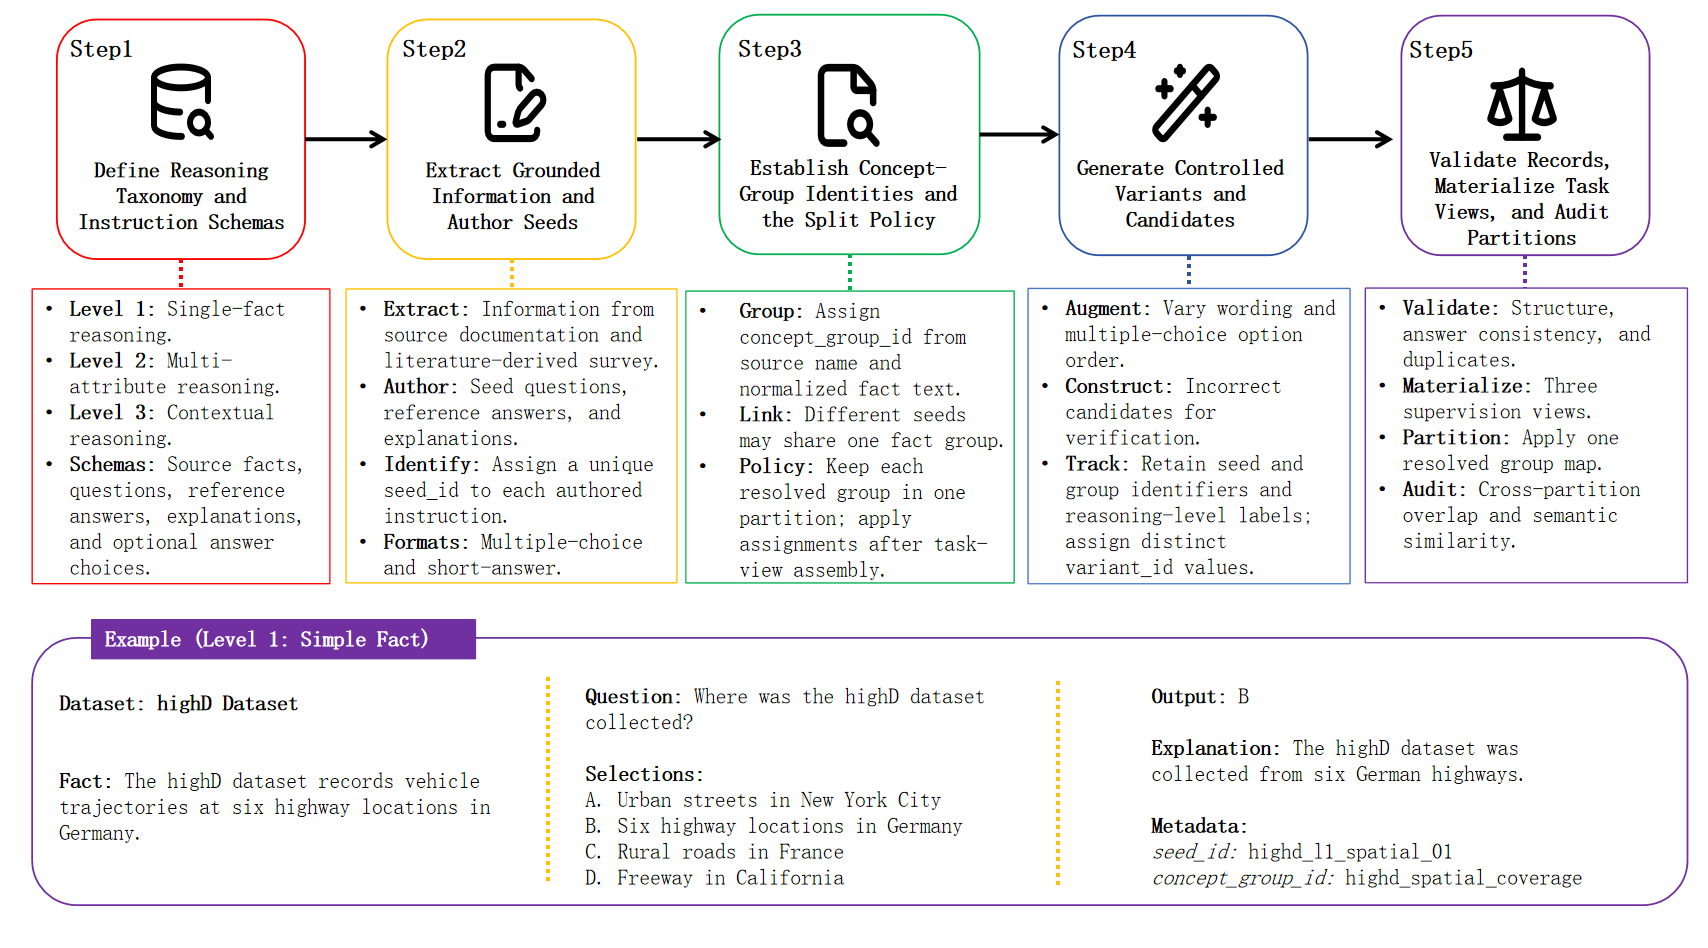
\includegraphics[width=\textwidth]{plots/urban_planning_llm_02.png}
%     \caption{Construction workflow for UrbanMobility-Instruct.
% Reasoning levels and instruction schemas guide source-grounded
% seed authoring. Seed and concept-group identities support
% controlled augmentation and structural validation. Validated
% records are materialized into complementary supervision views,
% assigned through a shared resolved concept-group map, and
% audited for cross-partition leakage. The lower panel illustrates
% a Level~1 multiple-choice seed grounded in the highD dataset. The identifiers \texttt{highd\_l1\_spatial\_01} and
% \texttt{highd\_spatial\_coverage} are illustrative labels
% for readability, not literal identifiers from the released
% corpus; actual group identifiers follow the source-and-hash
% construction and alias resolution described in Section~3.3.}
%     \label{fig:urban_llm_flowchart}
% \end{figure}

% \medskip
% \noindent\textbf{Step 1: Define Reasoning Taxonomy and Instruction Schemas.}

% We organize instructions into three reasoning levels:
% Level~1 (single-fact), Level~2 (multi-attribute), and Level~3
% (contextual reasoning). These levels distinguish whether a
% question requires direct retrieval of a documented property,
% integration of multiple properties, or interpretation of their
% analytical implications. The levels guide seed authoring and
% are retained as metadata during augmentation; they are not
% independently reassigned by the validation procedure.

% The common instruction schema contains a source fact, a
% question, a reference answer, and an explanation. Multiple-choice
% instructions additionally contain labeled answer options and
% identify the correct option. Multiple-choice and short-answer
% formats represent the underlying question--answer content,
% from which the supervision views described below are constructed.

% \textit{Level 1: Single-fact reasoning.}
% Level~1 targets direct understanding of explicitly documented
% source characteristics. To provide systematic coverage rather
% than selecting properties ad hoc, questions are organized around
% ten analytical perspectives: \textit{provenance},
% \textit{spatial coverage}, \textit{temporal coverage},
% \textit{measurement resolution}, \textit{variable definitions},
% \textit{file structure}, \textit{collection methodology},
% \textit{data accessibility and availability},
% \textit{usage context}, and \textit{dataset limitations}.
% Together, these perspectives describe where a source originates,
% what and where it measures, when and at what resolution
% observations are represented, how the data are collected and
% structured, how they can be accessed and used, and what
% limitations are documented. Each Level~1 question focuses on
% a single perspective and can be answered directly from the
% grounded source information without requiring relationships
% among multiple perspectives. For each primary source, one
% multiple-choice and one short-answer seed are authored from
% each perspective, yielding 20 Level~1 seeds per source.

% \textit{Level 2: Multi-attribute reasoning.}
% Level~2 extends the Level~1 perspectives by requiring multiple
% documented source characteristics to be considered jointly.
% Questions are constructed from meaningful combinations of
% perspectives rather than isolated properties, requiring
% relationships among attributes such as spatial and temporal
% coverage, measurement resolution and variable definitions,
% or collection methodology and dataset limitations. Level~2
% therefore tests whether complementary source characteristics
% can be integrated while remaining within the information
% documented for that source.

% \textit{Level 3: Contextual reasoning.}
% Level~3 extends these relationships to their analytical
% implications. Questions use documented source characteristics,
% often spanning multiple perspectives, to reason about what
% a source may enable, constrain, or imply for a specified
% analytical objective. For example, a question may relate
% temporal resolution and available variables to the suitability
% of a source for examining a mobility phenomenon, or relate
% collection design and spatial coverage to limitations on the
% conclusions that can be drawn. Level~3 remains bounded by
% the supplied source information and does not require numerical
% inference over raw observations, geospatial computation,
% or independent professional planning judgment.

% \medskip
% \noindent\textbf{Step 2: Extract Grounded Information and Author Seeds.}

% We use the taxonomy and schemas defined in Step~1 to author
% seed instructions from the documentation of the four empirical
% sources and the literature-derived Urban Flow Prediction Survey.
% Each seed links a question, reference answer, and explanation
% to its supporting source information, reasoning level, and
% question format. Source grounding is established during seed
% authoring; the subsequent automated checks assess the
% structural and consistency properties described in Step~5.

% Each authored instruction receives a unique \texttt{seed\_id}.
% This identifier distinguishes individual seeds, including
% different question formats derived from the same source fact.
% The implementation also assigns a \texttt{concept\_group\_id},
% defined in Step~3, to identify the source-fact group used for
% partitioning. It does not maintain a separate
% \texttt{concept\_id} field. Originals and augmented descendants
% receive distinct \texttt{variant\_id} values while retaining
% their originating seed and group identifiers.

% The five primary sources contribute 160 authored seeds.
% France and Japan contribute 66 additional seeds constructed
% using the same procedure and reserved entirely for
% cross-regional evaluation.

% \medskip
% \noindent\textbf{Step 3: Establish Concept-Group Identities and the Split Policy.}

% To reduce leakage between training and evaluation, the split
% unit is a source-grounded fact group rather than an individual
% instruction or augmented record
% \cite{kaufman2012leakage}. During seed preparation, a
% \texttt{concept\_group\_id} is derived from the source name
% and a hash of the normalized \texttt{Fact} text. Distinct
% \texttt{seed\_id} values can therefore share a
% \texttt{concept\_group\_id}, including multiple-choice and
% short-answer seeds grounded in the same normalized source fact.

% Before partition assignment, two documented alias mappings
% consolidate two pairs of reviewed equivalent fact groups:
% one pair from TLC Trip Records and one from Road Networks.
% Partitioning uses the resulting resolved group identifiers.
% Apart from these reviewed mappings, the groups are defined
% by normalized source facts and do not represent general
% semantic clusters of related knowledge.

% Group identities are available before augmentation, but
% partition assignment is performed subsequently on the
% assembled supervision views. The implementation constructs
% a single assignment map from the resolved groups and applies
% it consistently to generation, verification, and paraphrase
% records. Consequently, all seeds and descendants associated
% with a resolved group remain in one partition, without
% requiring partition files to exist before augmentation.

% As detailed in Section~4.1.1, the five primary sources are
% partitioned deterministically with random seed 2025 and an
% 80:10:10 target ratio, stratified by source. The 106 resolved
% groups yield 85 training, 11 validation, and 10 test groups
% (Table~\ref{tab:concept_split}). The target ratio applies to
% concept groups rather than augmented record counts.
% France and Japan are assigned entirely to the cross-regional
% holdout and do not participate in the primary split.


% \begin{table}[H]
% \centering
% \small
% \caption{Resolved concept-group assignments for the five-source
% primary corpus. A single assignment map is applied to the
% assembled supervision views after augmentation and structural
% validation.}
% \label{tab:concept_split}
% \begin{tabular}{lcc}
% \toprule
% \textbf{Partition} & \textbf{Concept Groups} & \textbf{Share} \\
% \midrule
% Training   & 85 & 80.2\% \\
% Validation & 11 & 10.4\% \\
% Test       & 10 & 9.4\% \\
% \midrule
% \textbf{Total} & \textbf{106} & \textbf{100.0\%} \\
% \bottomrule
% \end{tabular}
% \end{table}

% \medskip
% \noindent\textbf{Step 4: Generate Controlled Variants and Candidates.}

% GPT\mbox{-}5.1 \cite{openai2025gpt5} is used to expand the authored seeds into
% controlled instruction variants intended to preserve their
% source claims, task identity, and assigned reasoning level.
% This approach follows prior work on expanding
% instruction-tuning corpora through generated examples
% \cite{wang2023selfinstruct,taori2023alpaca}.
% Depending on task type and reasoning level, augmentation
% varies factual wording, question wording, answer and
% explanation wording, and multiple-choice option ordering.
% When options are reordered, the correct option label is
% updated accordingly.

% Every original and augmented canonical record retains its
% source, \texttt{seed\_id}, \texttt{concept\_group\_id},
% and reasoning level, and has a distinct \texttt{variant\_id}.
% Augmented records are descendants of existing seeds rather
% than new independent concepts. Their eventual partition
% membership is determined by the shared resolved group map
% described in Step~3.

% Each canonical record also carries an incorrect candidate
% intended to be inconsistent with the supplied source
% information. These candidates support the verification task;
% they are not used as desired answer-generation targets.
% Automated checks assess candidate distinctness and other
% consistency constraints, as described in Step~5, rather
% than independently certifying every candidate's factual status.


% \medskip
% \noindent\textbf{Step 5: Validate Records, Materialize Task Views, and Audit Partitions.}

% The assembled canonical records undergo automated structural
% and task-specific checks before task-view materialization.
% These checks cover required content and identifiers, valid
% multiple-choice answer labels, agreement between the selected
% option and stored answer text, exact duplicates, and
% separation of generation prompts from supervised targets.
% Candidate checks reject identical or excessively similar
% correct and incorrect answer texts under the implemented
% comparison rules.

% For short-answer records, a lexical-overlap heuristic flags
% weak surface correspondence between the reference answer
% and source fact. Such flags are warnings rather than
% automatic failures because valid reformulations may use
% different wording. Across the seven sources, all 14,726
% assembled canonical records pass the final structural gate,
% with zero rejected records and no exact duplicates.
% The heuristic flags 4,260 records, which are retained with
% warnings. These checks do not constitute independent factual
% verification of every generated claim, explanation, or
% incorrect candidate.

% The 14,726 canonical records comprise 10,560 records from
% the five primary sources and 4,166 records from the
% France--Japan holdout. Each canonical record produces one
% answer-generation example, so the canonical and generation
% totals describe corresponding records rather than additional
% independent pools. Table~\ref{tab:dataset_by_level} reports
% the primary-source subset.

% Validated records are materialized into three supervision views:

% \begin{itemize}
%     \item \textit{Answer generation.}
%     The input contains the source context, question, and
%     any answer options. The target contains the reference
%     answer and explanation.

%     \item \textit{Candidate verification.}
%     Each canonical record produces two examples: one
%     containing the reference answer as the supported
%     candidate and one containing the constructed incorrect
%     candidate. Their targets are the corresponding
%     \texttt{VERDICT} and
%     \texttt{CANDIDATE MATCHES CONTEXT} labels.
%     Incorrect candidates appear as inputs rather than
%     desired answer-generation outputs.

%     \item \textit{Structure-preserving paraphrase.}
%     Eligible augmented descendants are paired with their
%     completed original instructions. The original is the
%     input and the descendant is the target. Eligibility
%     requires the descendant's stored correct-answer value
%     to match that of the original. This is an operational
%     selection rule; it does not independently establish
%     complete semantic equivalence of all generated fields.
% \end{itemize}

% Across all seven sources, these transformations yield
% 14,726 generation, 29,452 verification, and 8,000 paraphrase
% examples. The five primary sources contribute 10,560,
% 21,120, and 5,580 examples, respectively; France and Japan
% contribute 4,166, 8,332, and 2,420. Verification and
% paraphrase examples are counted separately from canonical
% records, and all three views share seed and concept-group
% lineage.

% The assembled views are then assigned using the single
% resolved concept-group map. Deterministic leakage audits
% check resolved group overlap, seed overlap, and normalized
% exact generation-prompt overlap across the primary training,
% validation, and test partitions. All three checks report
% zero overlap.

% A separate semantic screen encodes generation prompts with
% \texttt{all-mpnet-base-v2}~\cite{allmpnetbasev2}, using
% the Sentence-BERT framework~\cite{reimers2019sentencebert}.
% Cross-partition pairs with cosine similarity of at least
% 0.90 are retained and deduplicated by concept pair for
% manual review. The France--Japan holdout is excluded from
% this screen. Three unique concept pairs are flagged and
% adjudicated as related but distinct because they require
% different answers or reasoning operations, leaving zero
% confirmed leakage cases among the reviewed pairs. This
% targeted review assesses potential cross-partition leakage,
% not the factual correctness of every corpus record.

% \begin{table}[H]
% \centering
% \caption{Validated answer-generation records from the five primary sources, reported by difficulty level and task type. France and Japan are excluded because they are reserved as cross-regional holdouts.}
% \label{tab:dataset_by_level}
% \resizebox{\columnwidth}{!}{%
% \renewcommand{\arraystretch}{1.15}
% \begin{tabular}{lcccccc}
% \toprule
% \textbf{Data Source} &
% \textbf{Level 1} &
% \textbf{Level 2} &
% \textbf{Level 3} &
% \textbf{SA} &
% \textbf{MC} &
% \textbf{Total} \\
% \midrule
% highD &
% 1,520 &
% 510 &
% 0 &
% 715 &
% 1,315 &
% 2,030 \\

% NGSIM &
% 1,520 &
% 510 &
% 0 &
% 715 &
% 1,315 &
% 2,030 \\

% Road Networks &
% 1,520 &
% 510 &
% 0 &
% 715 &
% 1,315 &
% 2,030 \\

% TLC Trip Records &
% 1,520 &
% 510 &
% 205 &
% 920 &
% 1,315 &
% 2,235 \\

% Urban Flow Prediction Survey &
% 1,520 &
% 510 &
% 205 &
% 920 &
% 1,315 &
% 2,235 \\
% \midrule

% \textbf{Total} &
% \textbf{7,600 (72.0\%)} &
% \textbf{2,550 (24.1\%)} &
% \textbf{410 (3.9\%)} &
% \textbf{3,985 (37.7\%)} &
% \textbf{6,575 (62.3\%)} &
% \textbf{10,560} \\
% \bottomrule
% \end{tabular}
% }
% \end{table}

% \begin{figure}[H]
%     \centering
%     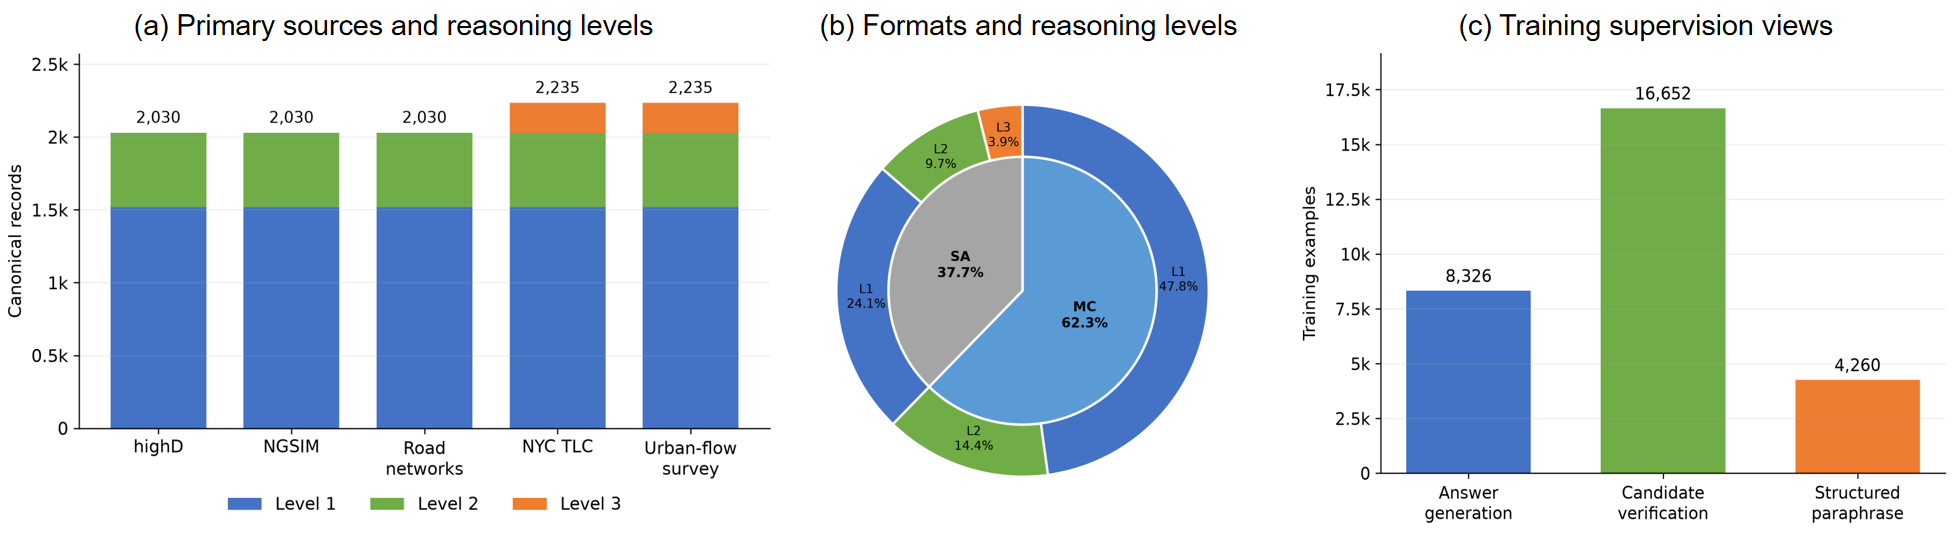
\includegraphics[width=\linewidth]{./plots/dataset_composition.png}
%     \caption{Composition of the primary-source instruction corpus and its training views. Panel~(a) reports the 10,560 canonical records by source and reasoning level. Panel~(b) summarizes the same records as a nested chart: the inner pie shows the multiple-choice (MC) and short-answer (SA) shares, and the outer ring shows the corresponding Level~1--3 composition. Panel~(c) reports the serialized examples in the training partition after materialization as answer-generation, candidate-verification, and structure-preserving paraphrase views. Candidate verification contains equal numbers of supported and unsupported candidates. The task views share canonical lineage and should not be interpreted as independent concepts.}
% \label{fig:sa_mc_level_distribution}
% \end{figure}

% \subsection{Held-Out Source Evaluation Construction}
% \label{sec:heldout-source-construction}

% To evaluate whether the learned source-grounded behavior transfers beyond the five primary sources used for fine-tuning, we construct additional evaluation data from two transportation sources: \textit{Île-de-France Mobilités Open Data} in France~\cite{idfm2024} and the \textit{Road Traffic Census} published by Japan's Ministry of Land, Infrastructure, Transport and Tourism (MLIT)~\cite{mlit2024}. Neither source contributes concepts or instruction records to model training. Instead, they introduce previously unseen source information and geographic contexts while retaining the same general instruction formulation used in the primary corpus. This setting therefore tests whether models can apply the learned reasoning and task structure to new source descriptions rather than only reproduce knowledge encountered during fine-tuning.

% The France and Japan evaluation sets are constructed from 66 separately authored seeds, with 33 seeds derived from each source. As in the primary corpus, the seeds are grounded in documented source information and formulated using the reasoning taxonomy introduced in Section~\ref{sec:dataset-construction}. Controlled variants are subsequently generated from these seeds while retaining their source and seed lineage. Because the purpose of this evaluation is transfer to unseen sources, all France- and Japan-derived records remain outside the primary training, validation, and test partitions.

% To distinguish transfer across source information from sensitivity to task formulation, the held-out records are represented using the same three supervision views as the primary corpus. The resulting evaluation data contain 4,166 answer-generation records, 8,332 candidate-verification records, and 2,420 structure-preserving paraphrase records. Candidate verification is balanced between supported and unsupported candidates, while paraphrase records retain the structural and answer-preservation constraints defined for the primary corpus. Across these views, records derived from the same authored seed remain linked through shared lineage and are therefore not interpreted as independent source concepts.

% The France--Japan evaluation is designed as a controlled held-out-source setting rather than a comprehensive test of geographic generalization. The sources introduce new geographic and source-specific information, but the questions follow the same reasoning taxonomy and controlled construction procedure as the primary corpus. Performance in this setting therefore measures transfer of the learned source-grounded task behavior to unseen source descriptions under a familiar instruction framework. A more independent test involving new sources, regions, and separately authored evaluation records is introduced in Section~\ref{sec:multiregional-benchmark}.

% \begin{table}[H]
% \centering
% \small
% \caption{Composition of the France--Japan held-out source evaluation. Counts for candidate verification include both supported and unsupported candidates.}
% \label{tab:france_japan_composition}
% \begin{tabular}{lc}
% \toprule
% \textbf{Component} & \textbf{Records} \\
% \midrule
% Authored seeds & 66 \\
% Answer generation & 4,166 \\
% Candidate verification & 8,332 \\
% Structure-preserving paraphrase & 2,420 \\
% \bottomrule
% \end{tabular}
% \end{table}

% \subsection{Multi-Regional External Benchmark Construction}
% \label{sec:multiregional-benchmark}

% To provide a more independent assessment of transfer beyond the controlled France--Japan setting, we construct a multi-regional external benchmark from ten additional transportation data sources spanning Australia, New Zealand, Brazil, Colombia, Ghana, Kenya, Spain, Greece, Iceland, and Sweden. None of these sources contributes records to model training or to the primary concept partitions. The benchmark introduces new source information and geographic contexts while retaining the core evaluation objective of determining whether a model can interpret documented source properties and reason about their supported implications.

% Unlike the primary corpus and the France--Japan evaluation sets, the benchmark is constructed directly as an evaluation resource rather than through large-scale augmentation of a smaller seed collection. For each of the ten sources, 35 records are independently authored from its documented information, producing 350 answer-generation records in total. These consist of 150 multiple-choice and 200 short-answer questions. The records follow the same broad reasoning framework used in the primary corpus, but their content is authored specifically for the external sources rather than generated as descendants of primary-corpus concepts. This construction reduces dependence on the augmentation process used for fine-tuning and provides a complementary test of behavior on newly introduced source information.

% Each answer-generation record is additionally transformed into one supported and one unsupported candidate-verification instance, yielding 700 balanced verification records. The supported candidate corresponds to the grounded answer, whereas the unsupported candidate conflicts with the documented source information. As in the primary corpus, incorrect candidates appear only as verification inputs and are never used as supervised target answers. Structure-preserving paraphrase records are not generated for this benchmark, because its purpose is to evaluate answer generation and verification on independently authored external content rather than transformation of augmented instruction variants.

% The benchmark is therefore complementary to both the primary held-out test partition and the France--Japan evaluation. The primary test partition isolates unseen concepts within the original five-source setting, whereas France and Japan introduce unseen source information and geographic contexts under the same controlled construction procedure. The ten-source benchmark further changes the source pool and relies on independently authored evaluation records without augmentation descendants. Together, these settings separate concept-level generalization within the primary corpus from transfer to held-out sources and transfer to a broader set of independently constructed external source descriptions.


% \begin{table}[htbp]
% \centering
% \small
% \setlength{\tabcolsep}{3pt}
% \renewcommand{\arraystretch}{1.2}
% \caption{Composition of the independent ten-source multi-regional
% benchmark. Each source contributes 15 multiple-choice and 20
% short-answer records. Each generation record produces one supported
% and one unsupported candidate-verification instance.}
% \label{tab:ten_dataset_composition}

% \begin{tabular}{@{}p{0.34\textwidth}p{0.13\textwidth}p{0.25\textwidth}rr@{}}
% \toprule
% \textbf{Dataset/source} &
% \textbf{Country} &
% \textbf{Data/source type} &
% \textbf{Generation} &
% \textbf{Verification} \\
% \midrule

% Melbourne Pedestrian Counting System
% \cite{melbournePedestrianHourly,melbournePedestrianSensors,melbournePedestrianMinute}
% & Australia
% & Pedestrian counts and sensor metadata
% & 35 & 70 \\

% Auckland Monthly Cycle Monitoring
% \cite{aucklandCycleMonitoring}
% & New Zealand
% & Automated bicycle counts
% & 35 & 70 \\

% Bogot\'a TransMilenio and SITP GTFS
% \cite{bogotaSITPGTFS}
% & Colombia
% & Public transport routes and schedules
% & 35 & 70 \\

% S\~ao Paulo Origin-Destination Survey 2017
% \cite{saopauloODSurvey,saopauloOD2017Report}
% & Brazil
% & Household travel survey
% & 35 & 70 \\

% Accra GTFS
% \cite{worldbankAccraGTFS}
% & Ghana
% & Public transport routes and schedules
% & 35 & 70 \\

% Nairobi Digital Matatus
% \cite{nairobiDigitalMatatus}
% & Kenya
% & Mapped minibus routes and stops
% & 35 & 70 \\

% Madrid Traffic Accidents
% \cite{madridTrafficAccidents}
% & Spain
% & Traffic crash records
% & 35 & 70 \\

% Athens Bus and Trolley Routes
% \cite{athensBusTrolleyGTFS}
% & Greece
% & Public transport routes and stops
% & 35 & 70 \\

% Vegager{\dh}in Traffic Statistics
% \cite{icelandTrafficStatistics}
% & Iceland
% & Road traffic counts and estimates
% & 35 & 70 \\

% Stockholm Open Traffic Data
% \cite{stockholmOpenTrafficData}
% & Sweden
% & Traffic data and network information
% & 35 & 70 \\

% \midrule
% \textbf{Total} & & & \textbf{350} & \textbf{700} \\
% \bottomrule
% \end{tabular}
% \end{table}

\section{Method}\label{sec4}
\subsection{Design Motivation and Framework Overview}

UrbanMobility-Instruct is designed to train and evaluate language models on source-grounded reasoning over documented urban-data characteristics. The framework organizes this capability into three reasoning levels: direct source comprehension, multi-attribute reasoning, and cross-dimensional interpretation. These levels progressively assess whether a model can identify individual source properties, establish relationships among documented characteristics, and interpret their implications for potential analytical use.

As illustrated in Figure~\ref{fig:urban_llm_flowchart}, the framework begins with source documentation and relevant literature, from which grounded facts and seed instructions are constructed. Seed and source-fact group identities are established before controlled augmentation, with lineage retained throughout the process. Following structural validation and materialization into answer-generation, candidate-verification, and structure-preserving paraphrase views, a shared resolved group map assigns related records to the same partition. This design reduces overlap between training and evaluation groups while supporting assessment on held-out concepts and geographically diverse sources.

\subsection{Source Selection and Grounding}
\label{sec:source-grounding}

The primary corpus is constructed from five complementary urban mobility and transportation knowledge sources. Four are empirical data resources: highD~\cite{highd2024dataset}, NGSIM~\cite{ngsim2024dataset}, Road Networks~\cite{networkrepository2024road}, and NYC TLC Trip Records~\cite{nyc2024tlc}. The fifth is a literature-derived source on urban flow prediction~\cite{xie2020urbanflow}. Together, these sources represent different forms of transportation information, including vehicle trajectories, road-network topology, trip activities, and urban-flow modeling concepts.

As summarized in Table~\ref{tab:source_characteristics}, the sources vary in observation unit, geographic coverage, spatial granularity, and temporal characteristics. This diversity supports the construction of instructions addressing different types of documented source properties and their analytical implications. Importantly, the framework operates on source documentation and relevant literature rather than directly processing raw trajectory, network, or trip data. Each authored instruction retains its source and underlying fact-group association, enabling provenance tracking during augmentation and dataset partitioning.

\begin{table}[H]
\centering
\small
\setlength{\tabcolsep}{4pt}
\renewcommand{\arraystretch}{1.2}
\caption{Characteristics of the five primary knowledge sources.}
\label{tab:source_characteristics}
\begin{tabular}{@{}>{\raggedright\arraybackslash}p{2.35cm}>{\raggedright\arraybackslash}p{3.55cm}>{\raggedright\arraybackslash}p{3.65cm}>{\raggedright\arraybackslash}p{3.5cm}@{}}
\toprule
\textbf{Source} & \textbf{Data type and unit} & \textbf{Spatial scope} & \textbf{Temporal scope} \\
\midrule
highD~\cite{highd2024dataset} & Drone trajectories; vehicle positions and maneuvers & Six highway locations in Germany & Frame-level recordings \\
NGSIM~\cite{ngsim2024dataset} & Video trajectories; vehicle positions and lane behavior & California road segments (I-80, US~101) & 0.1-second intervals \\
Road Networks~\cite{networkrepository2024road} & Graphs; road vertices and edges & Regional networks (e.g., CA, PA) & Static snapshots \\
NYC TLC~\cite{nyc2024tlc} & Taxi and for-hire trip records & NYC pickup/drop-off locations and zones & Trip timestamps; monthly files \\
Urban Flow Prediction Survey~\cite{xie2020urbanflow} & Literature synthesis; concepts and methods & Urban-flow studies across settings & Forecast horizons; no fixed interval \\
\bottomrule
\end{tabular}
\end{table}

% \subsection{Dataset Construction}
% \label{sec:dataset-construction}

% The corpus construction follows five stages: (1) define reasoning levels and instruction schemas; (2) author source-grounded seeds; (3) establish source-fact group identities; (4) generate controlled variants; and (5) validate records, materialize task views, and audit partitions (Figure~\ref{fig:urban_llm_flowchart}). Group identities are established before augmentation, while a shared resolved group map assigns partitions after view assembly.

% \begin{figure}[H]
%     \centering
%     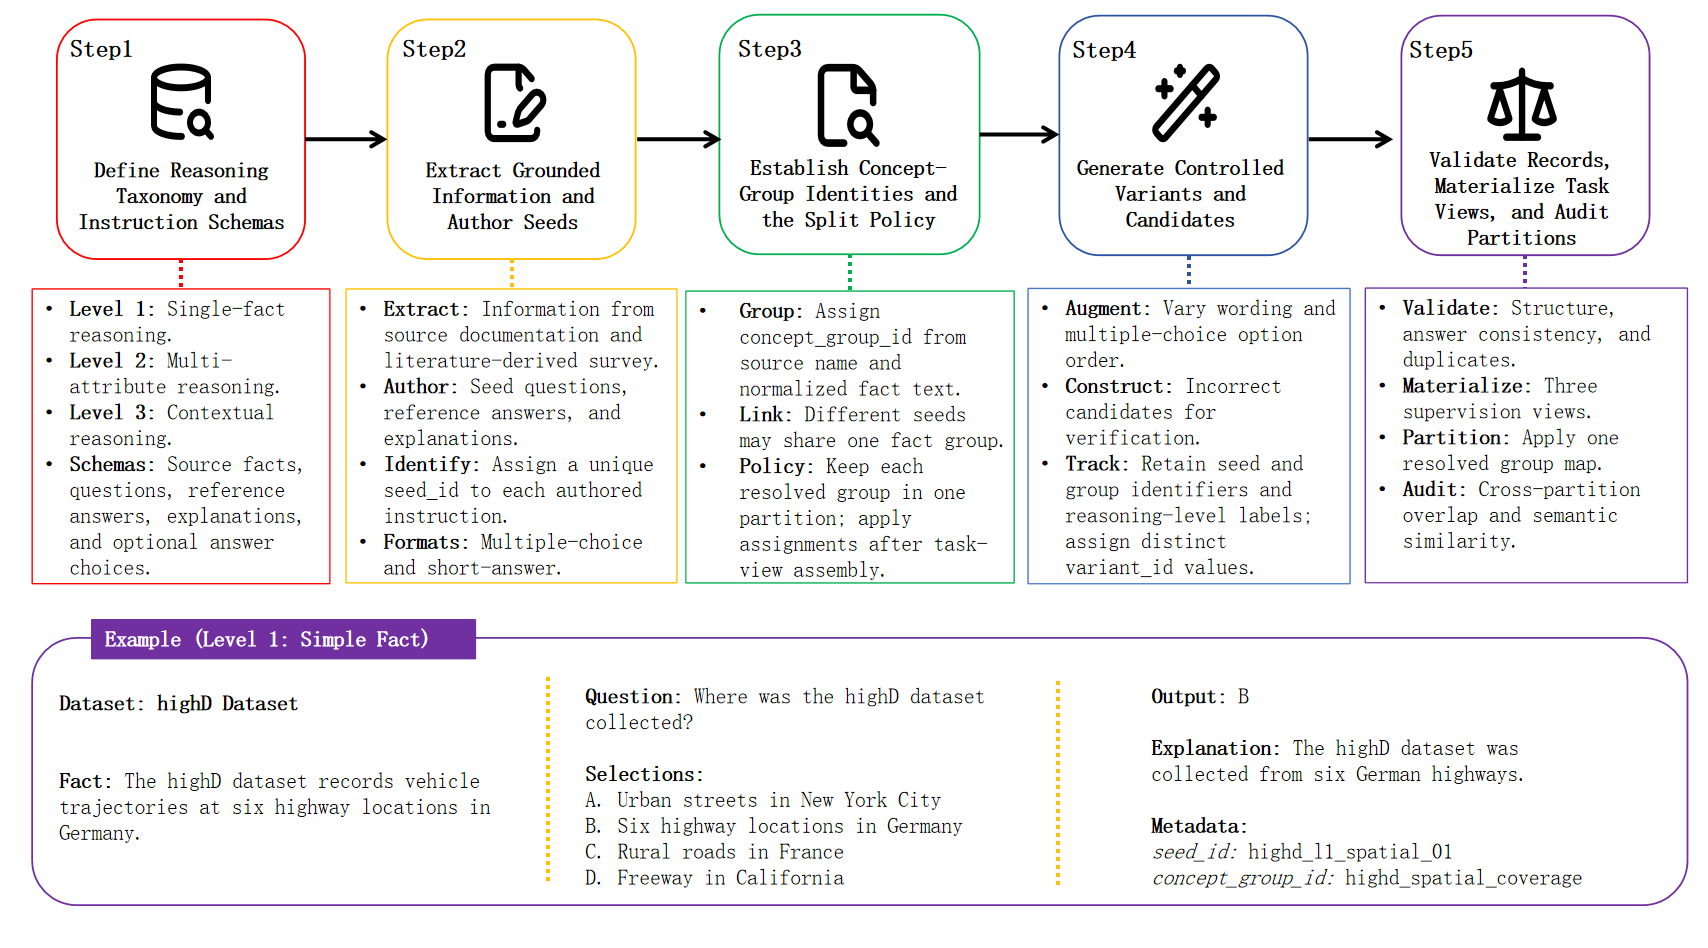
\includegraphics[width=\textwidth]{plots/urban_planning_llm_02.png}
%     \caption{UrbanMobility-Instruct construction workflow, from source-grounded seed authoring and augmentation to validation, supervision-view assembly, and concept-group-based partitioning. The lower panel shows an illustrative Level~1 highD multiple-choice example; its identifiers are schematic rather than actual corpus IDs.}
%     \label{fig:urban_llm_flowchart}
% \end{figure}

% \medskip
% \noindent\textbf{Step 1: Define Reasoning Taxonomy and Instruction Schemas.}

% Instructions are organized into three reasoning levels: Level~1 (single-fact), Level~2 (multi-attribute), and Level~3 (contextual reasoning). The levels guide seed authoring and are retained as metadata during augmentation. Each instruction contains a source fact, question, reference answer, and explanation; multiple-choice instructions additionally include labeled options and the correct option.

% \textit{Level 1: Single-fact reasoning.}
% Level~1 focuses on individual documented source properties across ten analytical perspectives: \textit{provenance}, \textit{spatial coverage}, \textit{temporal coverage}, \textit{measurement resolution}, \textit{variable definitions}, \textit{file structure}, \textit{collection methodology}, \textit{data accessibility and availability}, \textit{usage context}, and \textit{dataset limitations}. For each primary source, one multiple-choice and one short-answer seed are authored per perspective, yielding 20 Level~1 seeds per source.

% \textit{Level 2: Multi-attribute reasoning.}
% Level~2 requires integrating multiple documented source characteristics, such as spatial and temporal coverage or measurement resolution and variable definitions, to identify relationships among source properties.

% \textit{Level 3: Contextual reasoning.}
% Level~3 interprets the analytical implications of documented source characteristics, including their suitability and limitations for specified research objectives. Reasoning remains bounded by the supplied source information and does not require numerical analysis of raw observations, geospatial computation, or independent professional planning judgment.

% \medskip
% \noindent\textbf{Step 2: Extract Grounded Information and Author Seeds.}

% Using the taxonomy and schemas defined in Step~1, we author seed instructions from the four empirical sources and the literature-derived Urban Flow Prediction Survey. Each seed links its question, reference answer, and explanation to the supporting source information, reasoning level, and question format. A unique \texttt{seed\_id} identifies each instruction, while \texttt{concept\_group\_id} links seeds grounded in the same source-fact group for partitioning (Step~3). Originals and augmented descendants receive distinct \texttt{variant\_id} values while retaining their seed and group lineage. The five primary sources contribute 160 authored seeds, while France and Japan contribute 66 additional seeds reserved entirely for cross-regional evaluation.

% \medskip
% \noindent\textbf{Step 3: Establish Concept-Group Identities and the Split Policy.}

% We split by source-grounded fact group rather than by instruction row~\cite{kaufman2012leakage}. Each \texttt{concept\_group\_id} combines the source name with a hash of normalized \texttt{Fact} text, allowing distinct seeds, including multiple-choice and short-answer instructions grounded in the same fact, to share a group. Distinct multiple-choice and short-answer seeds grounded in the same normalized source fact can share a \texttt{concept\_group\_id} Two manually reviewed alias mappings merge equivalent groups (one TLC pair and one Road Networks pair); other groups are not general semantic clusters. After assembling the supervision views, one deterministic, source-stratified assignment map (seed 2025; target 80:10:10) assigns all descendants of each resolved group to the same partition. The 106 resolved groups yield 85 training, 11 validation, and 10 test groups (Table~\ref{tab:concept_split}); ratios apply to groups, not record counts. France and Japan remain entirely held out.

% \begin{table}[H]
% \centering
% \small
% \caption{Concept-group split of the five-source primary corpus.}
% \label{tab:concept_split}
% \begin{tabular}{lcc}
% \toprule
% \textbf{Partition} & \textbf{Groups} & \textbf{Share} \\
% \midrule
% Training   & 85 & 80.2\% \\
% Validation & 11 & 10.4\% \\
% Test       & 10 & 9.4\% \\
% \midrule
% \textbf{Total} & \textbf{106} & \textbf{100.0\%} \\
% \bottomrule
% \end{tabular}
% \end{table}

% \medskip
% \noindent\textbf{Step 4: Generate Controlled Variants and Candidates.}

% GPT\mbox{-}5.1~\cite{openai2025gpt5} expands authored seeds into controlled variants intended to preserve source claims, task identity, and reasoning level, following prior instruction augmentation approaches~\cite{wang2023selfinstruct,taori2023alpaca}. Depending on the task, augmentation varies source-fact wording, questions, answers, explanations, and multiple-choice option ordering, with correct labels updated accordingly. All variants retain their originating seed and concept-group lineage and receive distinct \texttt{variant\_id} values.

% Each canonical record also contains an incorrect candidate intended to contradict its source context for the candidate-verification task. These candidates are used only as verification inputs, not answer-generation targets. Structural and candidate-consistency checks are described in Step~5.


% \medskip
% \medskip
% \noindent\textbf{Step 5: Validate Records, Materialize Task Views, and Audit Partitions.}

% Canonical records undergo automated checks for required fields, identifiers, multiple-choice answer consistency, exact duplicates, prompt--target separation, and candidate distinctness. Candidate checks reject identical or excessively similar correct and incorrect answers under the implemented comparison rules. A lexical-overlap heuristic flags short answers with weak surface correspondence to their source facts without rejecting potentially valid reformulations. All 14,726 canonical records pass the structural checks without rejection or exact duplication, while 4,260 retain lexical-overlap warnings. These checks do not independently verify the factual correctness of generated claims, explanations, or incorrect candidates.

% The validated records comprise 10,560 primary-source and 4,166 France--Japan holdout records. Each canonical record yields one answer-generation example. Three complementary supervision views are materialized:

% \begin{itemize}
%     \item \textit{Answer generation.}
%     The model predicts the reference answer and explanation from the source context, question, and optional answer choices.

%     \item \textit{Candidate verification.}
%     Each record yields one supported and one unsupported candidate, with corresponding \texttt{VERDICT} and \texttt{CANDIDATE MATCHES CONTEXT} targets. Incorrect candidates appear only as verification inputs.

%     \item \textit{Structure-preserving paraphrase.}
%     Eligible augmented descendants are paired with their completed original instructions, using the original as input and the descendant as target. Eligibility requires matching stored correct-answer values, which does not independently guarantee complete semantic equivalence.
% \end{itemize}

% Across all seven sources, the views contain 14,726 generation, 29,452 verification, and 8,000 paraphrase examples. The primary sources contribute 10,560, 21,120, and 5,580 examples, respectively; France and Japan contribute 4,166, 8,332, and 2,420. All views retain shared seed and concept-group lineage, and their records do not represent independent source concepts.

% A single resolved concept-group map assigns the assembled views to partitions. Deterministic leakage audits find zero overlap in resolved groups, seeds, and normalized exact generation prompts across primary training, validation, and test partitions.

% For semantic screening, generation prompts are encoded using \texttt{all-mpnet-base-v2}~\cite{allmpnetbasev2} within the Sentence-BERT framework~\cite{reimers2019sentencebert}. Cross-partition pairs with cosine similarity $\geq 0.90$ are deduplicated by concept pair and manually reviewed. The France--Japan holdout is excluded. Three flagged concept pairs are judged related but distinct because they require different answers or reasoning operations, yielding zero confirmed leakage cases among reviewed pairs. This targeted audit does not establish the factual correctness of all corpus records or rule out every possible form of conceptual overlap.


% \begin{table}[H]
% \centering
% \caption{Answer-generation records by source, difficulty level, and task type.}
% \label{tab:dataset_by_level}
% \resizebox{\columnwidth}{!}{%
% \renewcommand{\arraystretch}{1.15}
% \begin{tabular}{lcccccc}
% \toprule
% \textbf{Source} &
% \textbf{Level 1} &
% \textbf{Level 2} &
% \textbf{Level 3} &
% \textbf{SA} &
% \textbf{MC} &
% \textbf{Total} \\
% \midrule
% highD & 1,520 & 510 & 0 & 715 & 1,315 & 2,030 \\
% NGSIM & 1,520 & 510 & 0 & 715 & 1,315 & 2,030 \\
% Road Networks & 1,520 & 510 & 0 & 715 & 1,315 & 2,030 \\
% NYC TLC & 1,520 & 510 & 205 & 920 & 1,315 & 2,235 \\
% Urban Flow Survey & 1,520 & 510 & 205 & 920 & 1,315 & 2,235 \\
% \midrule
% \textbf{Total} &
% \textbf{7,600 (72.0\%)} &
% \textbf{2,550 (24.1\%)} &
% \textbf{410 (3.9\%)} &
% \textbf{3,985 (37.7\%)} &
% \textbf{6,575 (62.3\%)} &
% \textbf{10,560} \\
% \bottomrule
% \end{tabular}
% }
% \end{table}

% \begin{figure}[H]
%     \centering
%     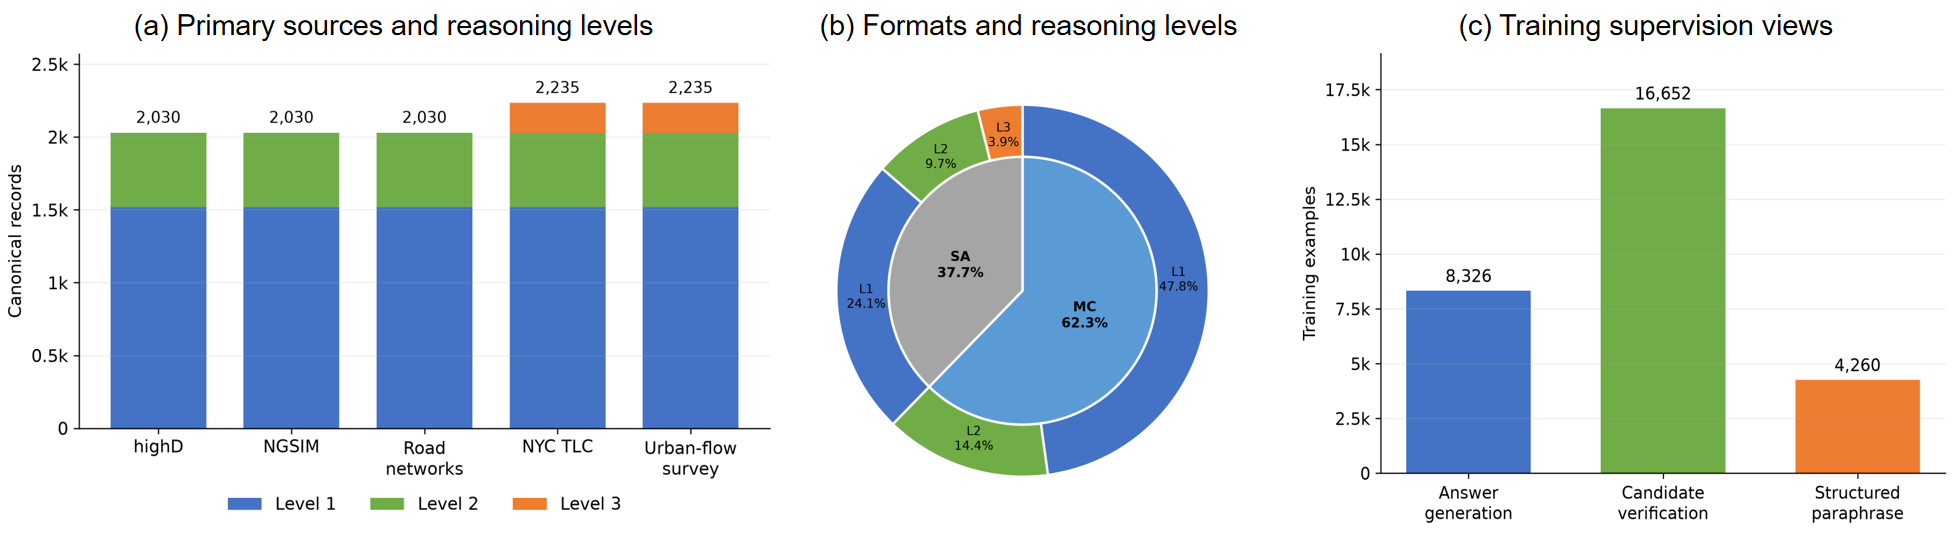
\includegraphics[width=\linewidth]{./plots/dataset_composition.png}
%     \caption{Primary-corpus composition and training views. Panels~(a)--(b) show the 10,560 canonical records by source, reasoning level, and task type (MC/SA); panel~(c) shows the materialized training examples across generation, verification, and paraphrase views.}
%     \label{fig:sa_mc_level_distribution}
% \end{figure}

\subsection{Dataset Construction}
\label{sec:dataset-construction}

UrbanMobility-Instruct is constructed from documented source information through five stages: defining reasoning levels and instruction schemas, authoring grounded seeds, establishing concept-group identities, generating controlled variants, and validating and materializing supervision views. Group identities are established before augmentation, whereas partition assignments are applied after task-view assembly using a shared resolved concept-group map. Figure~\ref{fig:urban_llm_flowchart} illustrates the workflow.

\begin{figure}[H]
    \centering
    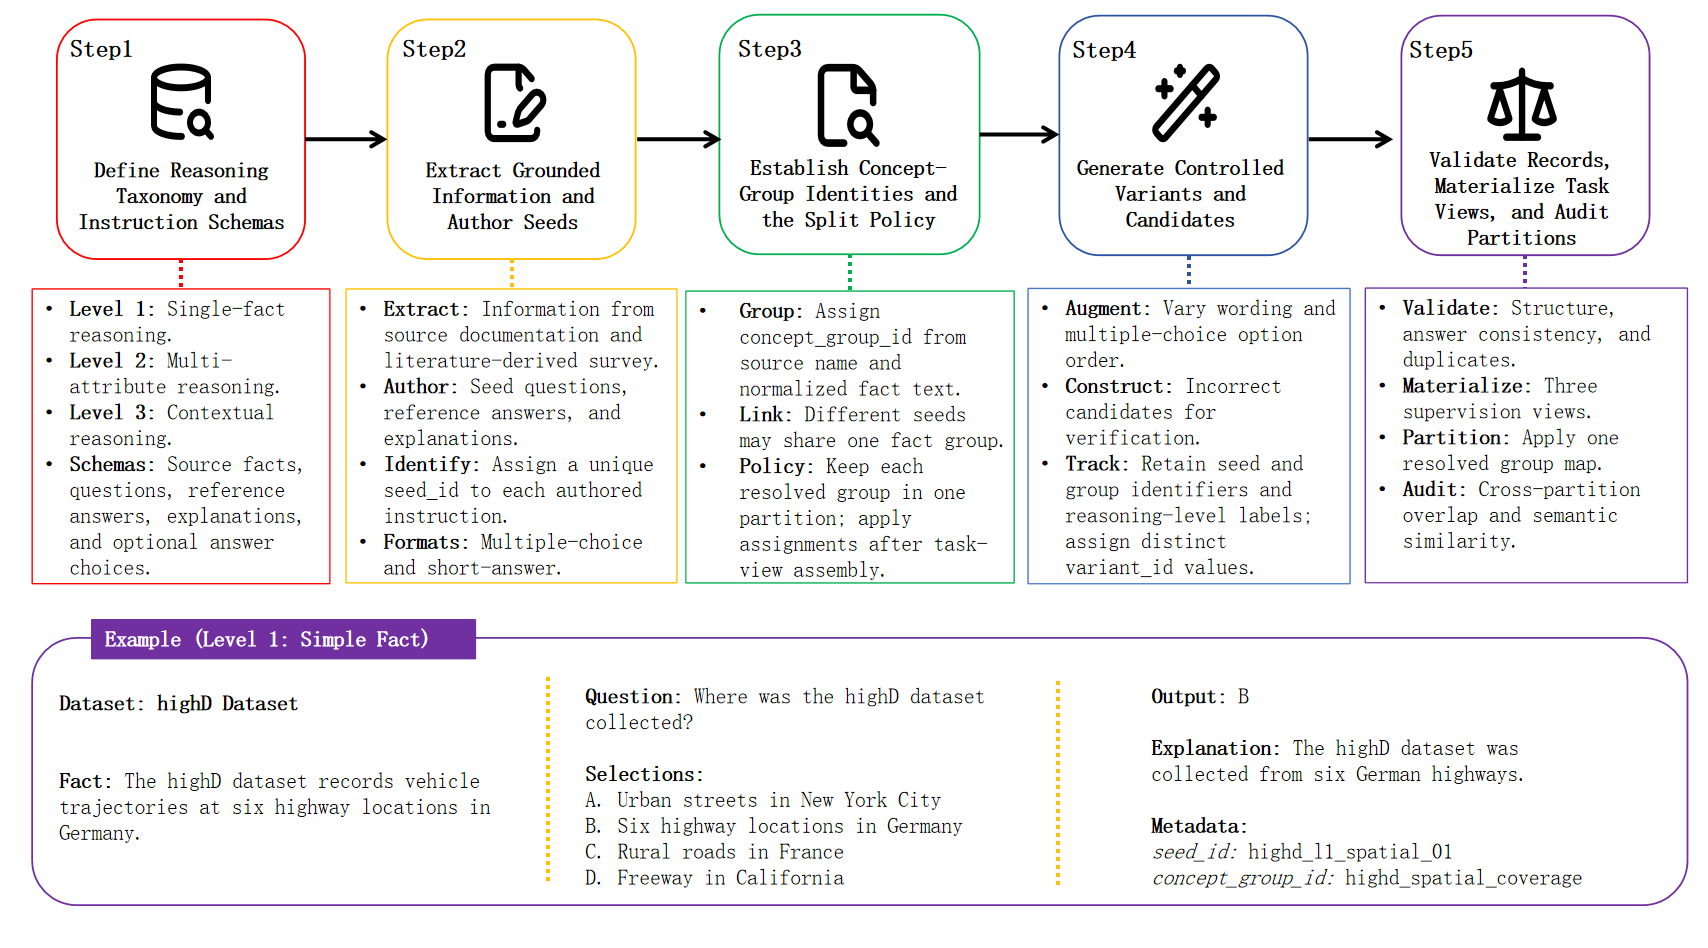
\includegraphics[width=\textwidth]{plots/urban_planning_llm_02.png}
    \caption{Construction workflow for UrbanMobility-Instruct. Reasoning levels and instruction schemas guide grounded seed authoring, followed by concept-group identification, controlled augmentation, structural validation, task-view materialization, and partition auditing. A shared resolved concept-group map assigns all related records to the same partition. The lower panel illustrates a Level~1 multiple-choice seed grounded in highD. The identifiers \texttt{highd\_l1\_spatial\_01} and \texttt{highd\_spatial\_coverage} are illustrative rather than literal corpus identifiers; actual group identifiers follow the source-and-hash construction and alias resolution described below.}
    \label{fig:urban_llm_flowchart}
\end{figure}

\medskip
\noindent\textbf{Step 1: Define Reasoning Taxonomy and Instruction Schemas.}

Instructions follow three reasoning levels: Level~1 (single-fact), Level~2 (multi-attribute), and Level~3 (contextual reasoning), progressing from identifying documented properties to integrating multiple characteristics and interpreting their analytical implications. Reasoning levels are assigned during seed authoring and retained throughout augmentation.

Each instruction contains a source fact, question, reference answer, and explanation. Multiple-choice (MC) instructions additionally include labeled options and a correct-option label, while short-answer (SA) instructions require a textual response. Both formats support the subsequent supervision views.

\textit{Level 1: Single-fact reasoning.}
Level~1 addresses ten documented source perspectives: \textit{provenance}, \textit{spatial coverage}, \textit{temporal coverage}, \textit{measurement resolution}, \textit{variable definitions}, \textit{file structure}, \textit{collection methodology}, \textit{data accessibility and availability}, \textit{usage context}, and \textit{dataset limitations}. Each question targets one perspective without requiring cross-attribute reasoning. One MC and one SA seed per perspective yield 20 Level~1 seeds per primary source.

\textit{Level 2: Multi-attribute reasoning.}
Level~2 integrates multiple documented characteristics, such as spatial and temporal coverage or measurement resolution and variable definitions, to examine relationships among source attributes.

\textit{Level 3: Contextual reasoning.}
Level~3 interprets the analytical implications of documented characteristics, such as how temporal resolution and available variables affect analytical suitability or how collection design constrains conclusions. Reasoning remains grounded in source documentation without requiring raw-data computation or independent planning judgment. Five Level~3 SA seeds are authored for each of TLC Trip Records and the Urban Flow Prediction Survey, whose documented evidence supports broader cross-dimensional reasoning. The other three sources are excluded from Level~3 seed authoring to avoid unsupported complexity.

\medskip
\noindent\textbf{Step 2: Extract Grounded Information and Author Seeds.}

Using the taxonomy and schemas in Step~1, we author seeds from the documentation of four empirical sources and the literature-derived Urban Flow Prediction Survey. Each seed links its question, reference answer, and explanation to supporting source information, reasoning level, and question format. Grounding is established during authoring; subsequent automated checks assess structural and consistency properties rather than independently verifying every factual claim.

Each authored instruction receives a unique \texttt{seed\_id}. Different seeds, including MC and SA questions grounded in the same source fact, may share a \texttt{concept\_group\_id} as defined in Step~3. The implementation does not maintain a separate \texttt{concept\_id} field. Originals and augmented descendants receive distinct \texttt{variant\_id} values while retaining their originating seed and group identifiers.

The five primary sources contribute 160 authored seeds. An additional 66 seeds from France and Japan are constructed using the same procedure and reserved entirely for cross-regional evaluation.

\medskip
\noindent\textbf{Step 3: Establish Concept-Group Identities and the Split Policy.}

To prevent cross-partition leakage, we split by source-grounded fact groups rather than individual records~\cite{kaufman2012leakage}. Each \texttt{concept\_group\_id} combines the source name with a hash of normalized \texttt{Fact} text, allowing MC and SA seeds grounded in the same fact to share a group. Two manually reviewed alias mappings merge equivalent group pairs (one TLC and one Road Networks); otherwise, grouping follows normalized facts rather than broad semantic similarity.

Group identities are established before augmentation, while partition assignments are applied after structural validation and supervision-view materialization. A single resolved group-assignment map keeps all seeds and descendants together across generation, verification, and paraphrase views.

The 106 resolved primary-source groups are split deterministically by source using random seed 2025 and an 80:10:10 target ratio, yielding 85 training, 11 validation, and 10 test groups (Table~\ref{tab:concept_split}; Section~4.1.1). Ratios apply to groups rather than augmented records. France and Japan remain entirely held out.

\begin{table}[H]
\centering
\small
\caption{Resolved concept-group assignments for the five-source primary corpus.}
\label{tab:concept_split}
\begin{tabular}{lcc}
\toprule
\textbf{Partition} & \textbf{Concept Groups} & \textbf{Share} \\
\midrule
Training   & 85 & 80.2\% \\
Validation & 11 & 10.4\% \\
Test       & 10 & 9.4\% \\
\midrule
\textbf{Total} & \textbf{106} & \textbf{100.0\%} \\
\bottomrule
\end{tabular}
\end{table}

\medskip
\noindent\textbf{Step 4: Generate Controlled Variants and Candidates.}

GPT\mbox{-}5.1~\cite{openai2025gpt5} expands the authored seeds into controlled instruction variants intended to preserve their source claims, task identity, and reasoning level. This follows prior work on instruction-data expansion~\cite{wang2023selfinstruct,taori2023alpaca}. Depending on the task type and level, augmentation varies source-fact wording, question wording, reference answers, explanations, and MC option ordering. Correct-option labels are updated whenever options are reordered.

Each original and augmented canonical record retains its source, \texttt{seed\_id}, \texttt{concept\_group\_id}, and reasoning level, together with a distinct \texttt{variant\_id}. Augmented records remain descendants of existing seeds rather than independent concepts, and their partition membership follows the resolved group map.

Each canonical record also includes an incorrect candidate intended to conflict with the supplied source information. These candidates support candidate verification and are never used as desired answer-generation targets. Automated consistency checks assess candidate distinctness without independently certifying every candidate's factual status.

\medskip
\noindent\textbf{Step 5: Validate Records, Materialize Task Views, and Audit Partitions.}

Canonical records undergo automated validation before task-view materialization. Checks cover required fields and identifiers, MC answer-label consistency, exact duplicates, separation of generation prompts and targets, and correct--incorrect candidate distinctness. For SA records, a lexical-overlap heuristic flags weak correspondence between reference answers and source facts without automatically rejecting valid reformulations. All 14,726 assembled canonical records pass the final structural gate, with zero rejections at that stage and no exact duplicates; 4,260 lexical warnings are retained. These checks do not independently establish factual correctness.

The corpus comprises 10,560 primary-source and 4,166 France--Japan canonical records, each corresponding to one answer-generation example. Table~\ref{tab:dataset_by_level} summarizes the primary subset. Validated records produce three supervision views:

\begin{itemize}
    \item \textit{Answer generation.}
    Source context, question, and optional answer choices form the input; the reference answer and explanation form the target.

    \item \textit{Candidate verification.}
    Each record yields one supported and one unsupported candidate, supervised by \texttt{VERDICT} and \texttt{CANDIDATE MATCHES CONTEXT} labels. Incorrect candidates are verification inputs, not generation targets.

    \item \textit{Structure-preserving paraphrase.}
    Eligible augmented descendants are paired with completed original instructions as targets and inputs, respectively. Eligibility requires matching stored correct answers but does not guarantee full semantic equivalence.
\end{itemize}

Across seven sources, the views contain 14,726 generation, 29,452 verification, and 8,000 paraphrase examples. The primary sources contribute 10,560, 21,120, and 5,580 examples, respectively; France and Japan contribute 4,166, 8,332, and 2,420. All views retain shared seed and concept-group lineage rather than representing independent concepts.

After materialization, a shared resolved group map assigns records to partitions. Deterministic audits find zero cross-partition overlap in resolved groups, seeds, or normalized exact generation prompts across the primary train, validation, and test sets.

A complementary semantic screen uses \texttt{all-mpnet-base-v2}~\cite{allmpnetbasev2} within Sentence-BERT~\cite{reimers2019sentencebert} to identify cross-partition generation-prompt pairs with cosine similarity $\geq 0.90$. Flagged pairs are deduplicated by concept pair and manually reviewed, excluding the France--Japan holdout. Three unique concept pairs are identified and judged related but distinct because they require different answers or reasoning operations, yielding zero confirmed leakage cases among reviewed pairs. This audit does not verify individual record correctness.

\begin{table}[H]
\centering
\caption{Validated primary-source answer-generation records by reasoning level and question format. France and Japan are excluded.}
\label{tab:dataset_by_level}
\resizebox{\columnwidth}{!}{%
\renewcommand{\arraystretch}{1.15}
\begin{tabular}{lcccccc}
\toprule
\textbf{Data Source} &
\textbf{Level 1} &
\textbf{Level 2} &
\textbf{Level 3} &
\textbf{SA} &
\textbf{MC} &
\textbf{Total} \\
\midrule
highD & 1,520 & 510 & 0 & 715 & 1,315 & 2,030 \\
NGSIM & 1,520 & 510 & 0 & 715 & 1,315 & 2,030 \\
Road Networks & 1,520 & 510 & 0 & 715 & 1,315 & 2,030 \\
TLC Trip Records & 1,520 & 510 & 205 & 920 & 1,315 & 2,235 \\
Urban Flow Prediction Survey & 1,520 & 510 & 205 & 920 & 1,315 & 2,235 \\
\midrule
\textbf{Total} &
\textbf{7,600 (72.0\%)} &
\textbf{2,550 (24.1\%)} &
\textbf{410 (3.9\%)} &
\textbf{3,985 (37.7\%)} &
\textbf{6,575 (62.3\%)} &
\textbf{10,560} \\
\bottomrule
\end{tabular}
}
\end{table}

\begin{figure}[H]
    \centering
    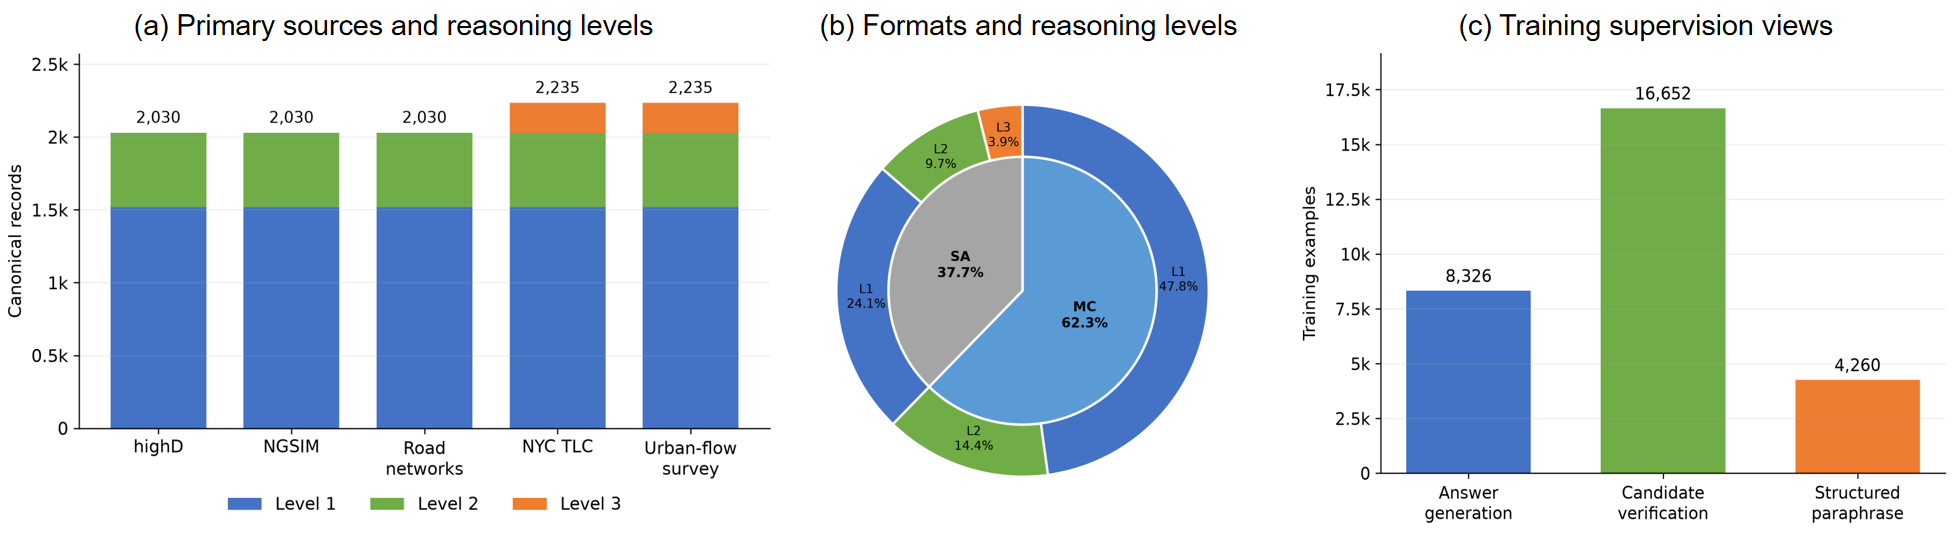
\includegraphics[width=\linewidth]{./plots/dataset_composition.png}
    \caption{Primary-source corpus composition and training views. Panel~(a) shows 10,560 canonical records by source and reasoning level; panel~(b) shows MC/SA shares and their level composition; panel~(c) shows generation, verification, and paraphrase examples in the training partition. Verification candidates are balanced, and all views share canonical lineage rather than independent concepts.}
    \label{fig:sa_mc_level_distribution}
\end{figure}

\subsection{Held-Out Source Evaluation Construction}
\label{sec:heldout-source-construction}

Cross-regional evaluation uses \textit{Île-de-France Mobilités Open Data}~\cite{idfm2024} and Japan's \textit{MLIT Road Traffic Census}~\cite{mlit2024}. Neither source contributes seeds or instruction records to model training, validation, or checkpoint selection. We author 33 source-grounded seeds per source and apply the same reasoning taxonomy, controlled augmentation, and task-view construction as the primary corpus. The resulting holdout contains 4,166 answer-generation, 8,332 balanced candidate-verification, and 2,420 structure-preserving paraphrase records (Table~\ref{tab:france_japan_composition}).

This setting tests whether the learned source-grounded behaviors transfer to previously unseen source information under familiar instruction formulations. However, augmented descendants share their originating seeds and concepts, and the two sources provide limited independent geographic coverage. Consequently, the evaluation is interpreted as controlled held-out-source transfer rather than unrestricted geographic generalization.

\begin{table}[H]
\centering
\small
\caption{Composition of the France--Japan held-out evaluation.}
\label{tab:france_japan_composition}
\begin{tabular}{lc}
\toprule
\textbf{Component} & \textbf{Records} \\
\midrule
Authored seeds & 66 \\
Answer generation & 4,166 \\
Candidate verification & 8,332 \\
Structure-preserving paraphrase & 2,420 \\
\bottomrule
\end{tabular}
\end{table}

\subsection{Multi-Regional External Benchmark Construction}
\label{sec:multiregional-benchmark}

To complement the controlled France--Japan evaluation, we construct an independent multi-regional benchmark from ten additional transportation sources spanning Australia, New Zealand, Brazil, Colombia, Ghana, Kenya, Spain, Greece, Iceland, and Sweden (Table~\ref{tab:ten_dataset_composition}). None of these sources contributes records to model training or checkpoint selection. Unlike the primary and France--Japan corpora, the benchmark is constructed directly from documented source information without large-scale augmentation. Each source contributes 35 independently authored records, yielding 350 answer-generation examples (150 multiple-choice and 200 short-answer) and 700 balanced candidate-verification instances. No paraphrase view is generated, as the benchmark evaluates answer generation and verification on independently authored records rather than transformations of augmented instructions.

The benchmark broadens both geographic and source-type coverage while reducing dependence on repeated variants of the same authored seeds. Its evaluation records use the same broad reasoning framework but are authored specifically for the external sources rather than derived from training-corpus concepts. Together, the three evaluation regimes distinguish generalization to held-out source-fact groups within the primary corpus, transfer to new sources under controlled augmentation, and transfer to independently authored questions from additional datasets.


\begin{table}[htbp]
\centering
\small
\setlength{\tabcolsep}{3pt}
\renewcommand{\arraystretch}{1.15}
\caption{Composition of the independent ten-source external benchmark.}
\label{tab:ten_dataset_composition}

\begin{tabular}{@{}p{0.34\textwidth}p{0.13\textwidth}p{0.25\textwidth}rr@{}}
\toprule
\textbf{Source} &
\textbf{Country} &
\textbf{Data type} &
\textbf{Generation} &
\textbf{Verification} \\
\midrule

Melbourne Pedestrian Counting System
\cite{melbournePedestrianHourly,melbournePedestrianSensors,melbournePedestrianMinute}
& Australia & Pedestrian counts and sensors & 35 & 70 \\

Auckland Monthly Cycle Monitoring
\cite{aucklandCycleMonitoring}
& New Zealand & Bicycle counts & 35 & 70 \\

Bogot\'a TransMilenio and SITP GTFS
\cite{bogotaSITPGTFS}
& Colombia & Transit routes and schedules & 35 & 70 \\

S\~ao Paulo Origin-Destination Survey 2017
\cite{saopauloODSurvey,saopauloOD2017Report}
& Brazil & Household travel survey & 35 & 70 \\

Accra GTFS
\cite{worldbankAccraGTFS}
& Ghana & Transit routes and schedules & 35 & 70 \\

Nairobi Digital Matatus
\cite{nairobiDigitalMatatus}
& Kenya & Minibus routes and stops & 35 & 70 \\

Madrid Traffic Accidents
\cite{madridTrafficAccidents}
& Spain & Traffic crash records & 35 & 70 \\

Athens Bus and Trolley Routes
\cite{athensBusTrolleyGTFS}
& Greece & Transit routes and stops & 35 & 70 \\

Vegager{\dh}in Traffic Statistics
\cite{icelandTrafficStatistics}
& Iceland & Road traffic statistics & 35 & 70 \\

Stockholm Open Traffic Data
\cite{stockholmOpenTrafficData}
& Sweden & Traffic and network data & 35 & 70 \\

\midrule
\textbf{Total} & & & \textbf{350} & \textbf{700} \\
\bottomrule
\end{tabular}
\end{table}


% \section{Experiments and Evaluations}
% This section evaluates whether dataset-centric instruction tuning improves grounded reasoning over urban-data source information, how its effects vary across model families, scales, tasks, and reasoning levels, and whether these effects generalize beyond the primary sources. We compare pretrained and fine-tuned T5, Qwen2.5, and Llama 3.1 models across answer correctness, grounded explanation quality, candidate verification and paired consistency, and answer and field preservation under structure-preserving paraphrase. Generalization is evaluated progressively on in-domain data from held-out resolved source-fact groups, geographically held-out French and Japanese sources with controlled question variants, and a ten-dataset multi-regional benchmark containing new source information and geographic contexts. Because augmented descendants share underlying seeds and concepts, row-level results are supplemented with a regional seed-macro multiple-choice sensitivity check for fine-tuned T5-base and external source-variation diagnostics for fine-tuned Llama 3.1-70B. The models serve as evaluation instruments rather than architectural contributions, assessing the utility and limitations of the constructed instruction corpus.

% \subsection{Evaluation Setup}
% \subsubsection{Dataset Splits and Formatting}
% Model development uses the five-source primary corpus described in Section~3. Each canonical record is grounded in documented source information and adopts one of two answer formats. A short-answer record contains a contextual fact, a question, a concise reference answer, and a grounded explanation. A multiple-choice record adds four labeled selections and identifies exactly one correct option. These two formats define the underlying question-answer content; they should not be confused with the three supervision views materialized from that content.

% \paragraph{Supervision Views}
% Each validated canonical record produces one \emph{answer-generation} example, in which the model predicts the correct answer and explanation from the context, question, and any options. It also produces two \emph{candidate-verification} examples: one supplies the supported answer and the other a plausible but source-inconsistent candidate. The required targets are respectively \texttt{Correct/Yes} and \texttt{Incorrect/No}. Incorrect candidates are therefore used only as inputs to a balanced discrimination task and never as desired generation outputs. Finally, eligible augmented descendants produce a \emph{structure-preserving paraphrase} example that maps a completed original instruction to a reformulated descendant. The model is instructed to preserve field labels, facts, option--answer relationships, answers, and explanation meaning. Eligibility requires the descendant's stored correct-answer value to equal the original value. This criterion and the structural checks described in Section~3 do not independently establish complete semantic equivalence. The training split contains 8,326 answer-generation examples, 16,652 verification examples, and 4,260 paraphrase examples. Because these views derive from shared canonical records, their counts do not represent independent concepts.

% \paragraph{Dataset Partitions}
% The five primary sources are partitioned deterministically using an 80:10:10 target ratio and random seed 2025. The indivisible split unit is the resolved \texttt{concept\_group\_id}: all seeds, task forms, and generated descendants associated with the same resolved source-fact group remain in one partition. Initial group identifiers are derived from the source name and a hash of normalized \texttt{Fact} text. Different seed identifiers can share a group, and two reviewed alias mappings consolidate equivalent fact groups. Beyond these aliases, the implementation does not construct general semantic clusters. Assignment is stratified by source, with integer allocations within each source and remaining groups assigned to meet the global partition totals. Task type and reasoning level are not separate stratification variables in this implementation; concepts can span multiple task forms and levels, and their integrity takes priority over matching those marginal distributions. The resulting 106 concept groups comprise 85 training, 11 validation, and 10 in-domain test groups: these are counts, corresponding to 80.19\%, 10.38\%, and 9.43\%, respectively. Specifically, the implementation rounds $0.8\times106$ to 85 training groups and $0.1\times106$ to 11 validation groups, then assigns the remaining ten groups to testing. Thus, 80:10:10 is the target proportion, with small deviations required by integer group allocation. They yield 8,326, 1,036, and 1,198 answer-generation records, respectively; the target ratio applies to concept groups, not augmented row counts. Training records are used for supervised fine-tuning, validation records only for checkpoint selection, and the in-domain test partition is reserved for final evaluation.

% Seed and initial group identities are established before augmentation. After augmentation, structural validation, and task-view assembly, partition membership is determined through a single assignment map based on the resolved source-fact groups. The same map is applied to generation, verification, and paraphrase views, so augmentation never makes descendants independently eligible for different partitions. This procedure provides concept-group isolation without requiring partition files to be created before augmentation. The resulting difficulty-level coverage is uneven and is reported explicitly in the results.

% The saved split manifest records the group assignments and counts. The associated leakage audit checks concept identities, seed identities, and normalized generation prompts across the primary train, validation, and test partitions; all three checks report zero overlap. A separate semantic screen and manual adjudication, described in Section~3, identify no confirmed leakage among the three flagged concept pairs. These checks concern the primary partitions; the geographically held-out sources are excluded from this cross-split semantic screen. Passing these checks does not establish the absence of all possible conceptual similarity or embedded answer cues.

% France and Japan are reserved in their entirety as a geographically held-out cross-regional set and contribute 4,166 additional answer-generation records; neither their seeds nor their descendants enter fitting or checkpoint selection. The ten-dataset multi-regional benchmark is maintained as a second, fully external test regime containing new source information, questions, and geographic contexts. It is not included in the primary 80:10:10 partition or used for model development. This separation distinguishes within-source concept generalization, transfer to controlled variants from held-out regions, and transfer to entirely new datasets.

% \paragraph{Model Input Serialization}
% All task views are serialized into separate prompt and target fields before tokenization. For answer generation, the prompt contains the dataset context, question, and---for multiple-choice records---options labeled A--D; the target contains only the required \texttt{ANSWER} and \texttt{EXPLANATION} fields. For candidate verification, the prompt additionally contains the candidate answer and requests exactly two fields, \texttt{VERDICT} and \texttt{CANDIDATE MATCHES CONTEXT}; the target supplies the corresponding correct/incorrect and yes/no labels. For paraphrase, the prompt contains the completed source instruction plus an explicit preservation request, and the target is the completed answer-preserving descendant. Model-specific tokenization and chat wrappers are applied after serialization without changing this task content. The designated supervised target is serialized separately from the prompt. Answer generation requests an answer and explanation, whereas verification intentionally exposes the candidate to be judged and paraphrase intentionally exposes the completed source instruction. Prompt--target separation therefore describes the training interface; it does not establish that source or generated prompt text is free of answer cues.
% \newpage
% \begin{lstlisting}[style=Matlab-editor]
% PROMPT
% Dataset context: [contextual fact]
% Question: [question text]
% [Multiple-choice only] Selections:
% A: ...
% B: ...
% C: ...
% D: ...

% TARGET
% ANSWER: [output]
% EXPLANATION: [grounded explanation]
% \end{lstlisting}

% \textbf{Rationale.}
% Retaining the canonical answer format while materializing task-specific views separates the underlying urban-data concept from the behavior being supervised. The shared field markers provide a consistent interface across model families, while the three views test complementary capabilities: producing a grounded response, discriminating supported from unsupported candidates, and reformulating a completed instruction without semantic or structural drift.
% The following Level~1 highD example illustrates how one canonical record is materialized into the three supervision views. All views retain the originating seed identity and share the same resolved source-fact group assignment. The readable metadata labels in Figure~\ref{fig:urban_llm_flowchart} are illustrative rather than literal corpus identifiers; actual group identities follow the source-and-hash construction and alias resolution described above.

% \begin{quote}
% \small
% \noindent\textbf{Dataset Context:} The highD dataset is collected from six drone-monitored German highways.

% \noindent\textbf{Question:} Where was the highD dataset collected?

% \noindent\textbf{Options:} (A) Urban streets in New York City; (B) Six highway locations in Germany; (C) Rural roads in France; (D) Freeways in California.

% \noindent\textbf{Answer-generation target:} \texttt{ANSWER: B} \quad \texttt{EXPLANATION:} The highD dataset was collected from six drone-monitored German highways.

% \noindent\textbf{Positive verification:} Candidate answer: \emph{Six highway locations in Germany}. Target: \texttt{VERDICT: Correct}; \texttt{CANDIDATE MATCHES CONTEXT: Yes}.

% \noindent\textbf{Negative verification:} Candidate answer: \emph{Rural roads in France}. Target: \texttt{VERDICT: Incorrect}; \texttt{CANDIDATE MATCHES CONTEXT: No}.

% \noindent\textbf{Illustrative paraphrase objective:} The context may be reformulated as ``Drones recorded the highD data at six German highway sites,'' with instructions to preserve the field labels, question meaning, four options, correct option~B, and explanation meaning. This illustrates the requested behavior, not an additional semantic-validation guarantee.
% \end{quote}

% \subsubsection{Evaluation Backbones}

% We use five pretrained generative language models as evaluation backbones: T5-base~\cite{raffel2020exploring}, Qwen2.5-7B-Instruct and Qwen2.5-14B-Instruct~\cite{yang2024qwen25}, and Llama-3.1-8B-Instruct and Llama-3.1-70B-Instruct~\cite{grattafiori2024llama}. This selection combines an encoder--decoder text-to-text baseline with two decoder-only instruction-model families. The paired 7B/14B Qwen and 8B/70B Llama variants permit within-family comparisons across scale, while T5-base tests whether the same task design transfers to a substantially smaller and architecturally different model. Separate pretrained encoders are used only to calculate BERTScore and NLI entailment; they are neither fine-tuned nor treated as generative evaluation backbones.

% All five models receive the same concept-group training partition and the same three supervision views. Architecture-specific formatting is limited to the native tokenizer and, for decoder-only models, the checkpoint's chat template. T5-base is updated through full-parameter fine-tuning. The Qwen and Llama models are adapted using 4-bit QLoRA \cite{dettmers2023qlora}: base weights use NF4 and double quantization, and rank-16 LoRA \cite{hu2022lora} adapters with scaling factor 32 and dropout 0.05 are applied to the attention and feed-forward projection modules. The 7B--14B and Llama 8B runs quantize their base weights on load. The 70B run loads the published prequantized \texttt{unsloth/Meta-Llama-3.1-70B-Instruct-bnb-4bit} weights, derived from Llama 3.1-70B-Instruct, because the full-precision download exceeded Colab disk capacity. Its paired base and fine-tuned evaluations use this same weight source. For causal models, prompt tokens are masked from the loss so that optimization is performed only on the supervised response. These choices make the larger-model experiments computationally feasible while keeping the data partition, task content, and evaluation protocol fixed. The study evaluates adaptation behavior rather than proposing a new architecture or optimization algorithm.

% \begin{table}[H]
% \centering
% \caption{Generative evaluation backbones and adaptation methods. Parameter counts are the nominal model sizes. QLoRA models use 4-bit NF4 base weights and rank-16 adapters.}
% \label{tab:models_metrics}
% \resizebox{\columnwidth}{!}{%
% \begin{tabular}{lllll}
% \toprule
% \textbf{Evaluation backbone} & \textbf{Architecture} & \textbf{Size} & \textbf{Pretrained checkpoint} & \textbf{Adaptation} \\
% \midrule
% T5-base & Encoder--decoder & 220M & \texttt{t5-base} & Full fine-tuning \\
% Qwen2.5-7B & Decoder-only & 7B & \texttt{Qwen/Qwen2.5-7B-Instruct} & 4-bit QLoRA \\
% Qwen2.5-14B & Decoder-only & 14B & \texttt{Qwen/Qwen2.5-14B-Instruct} & 4-bit QLoRA \\
% Llama-3.1-8B & Decoder-only & 8B & \texttt{meta-llama/Meta-Llama-3.1-8B-Instruct} & 4-bit QLoRA \\
% Llama-3.1-70B & Decoder-only & 70B & \texttt{unsloth/Meta-Llama-3.1-70B-Instruct-bnb-4bit} & 4-bit QLoRA \\
% \bottomrule
% \end{tabular}%
% }
% \end{table}

% \subsubsection{Training and Reproducibility Configuration}

% Table~\ref{tab:training_configuration} summarizes the optimization settings recovered from the serialized training arguments of the evaluated runs. All five checkpoints were trained on the same released instruction corpus, with identical concept-group assignments and task-record counts. Cross-model comparisons remain descriptive because the runs differ in model family, initial alignment, scale, architecture-specific prompt rendering, and the weight-loading procedure used for the 70B model. Physical batch size refers to the number of examples processed per device in a single forward pass; effective batch size is the physical training batch size multiplied by the gradient-accumulation factor. All runs use a single GPU, bfloat16 computation, fused AdamW \cite{loshchilov2019decoupled}, a linear learning-rate schedule, and a maximum of one training epoch. Causal models use response-only loss. Input and target sequences are truncated to 512 and 384 tokens, respectively. T5-base uses a warm-up ratio of 0.10 and weight decay of 0.01, whereas the four causal models use a warm-up ratio of 0.03 and no weight decay.

% \begin{table}[H]
% \centering
% \caption{Optimization configuration of the evaluated model runs. Train and evaluation batch sizes are per-device physical batches; effective batch size includes gradient accumulation. Evaluation and saving intervals are measured in optimizer steps.}
% \label{tab:training_configuration}
% \resizebox{\columnwidth}{!}{%
% \begin{tabular}{lrrrrrrr}
% \toprule
% \textbf{Model} & \textbf{Learning rate} & \textbf{Train batch} & \textbf{Eval. batch} & \textbf{Accum.} & \textbf{Effective batch} & \textbf{Epoch cap} & \textbf{Eval./save interval} \\
% \midrule
% T5-base       & $2\times10^{-5}$ & 32 & 32 & 2 & 64 & 1 & 100 \\
% Qwen2.5-7B    & $1\times10^{-4}$ & 12 & 32 & 2 & 24 & 1 & 25 \\
% Qwen2.5-14B   & $5\times10^{-5}$ & 12 & 32 & 2 & 24 & 1 & 25 \\
% Llama-3.1-8B  & $1\times10^{-4}$ & 8  & 32 & 2 & 16 & 1 & 50 \\
% Llama-3.1-70B & $5\times10^{-5}$ & 6  & 4  & 3 & 18 & 1 & 25 \\
% \bottomrule
% \end{tabular}%
% }
% \end{table}

% The random seed is 42 for optimization and 2025 for dataset partitioning. Checkpoints are ranked by validation loss, and the lowest-loss checkpoint is restored before publication and downstream evaluation. Early stopping for the causal models uses a patience of four validation events and a minimum improvement threshold of 0.001; T5-base completes its single epoch. Table~\ref{tab:checkpoint_selection} records the observed selection outcome. Trainer runtime excludes model download, metric computation, and artifact upload. Models through 14B were trained on a 40-GB NVIDIA A100, whereas Llama-3.1-70B used an 80-GB NVIDIA A100.

% \begin{table}[H]
% \centering
% \caption{Checkpoint selection and training runtime for the evaluated published runs. The stopping epoch is the fraction of the one-epoch cap reached when training ended. ES denotes early stopping with patience four.}
% \label{tab:checkpoint_selection}
% \resizebox{\columnwidth}{!}{%
% \begin{tabular}{lrrrrll}
% \toprule
% \textbf{Model} & \textbf{Best step} & \textbf{Best val. loss} & \textbf{Stop step} & \textbf{Stop epoch} & \textbf{Stopping rule} & \textbf{Trainer runtime} \\
% \midrule
% T5-base       & 457 & 0.8002 & 457 & 1.000 & Epoch complete & 0.07 h \\
% Qwen2.5-7B    & 75  & 0.5184 & 175 & 0.144 & ES & 1.12 h \\
% Qwen2.5-14B   & 100 & 0.4903 & 200 & 0.164 & ES & 2.39 h \\
% Llama-3.1-8B  & 150 & 0.5170 & 350 & 0.192 & ES & 1.36 h \\
% Llama-3.1-70B & 100 & 0.4563 & 200 & 0.123 & ES & 8.98 h \\
% \bottomrule
% \end{tabular}%
% }
% \end{table}

% \subsection{Base-Model vs Fine-Tuned Comparison}

% For each backbone, we conduct a paired comparison between the unadapted checkpoint and the checkpoint obtained after supervised training on the proposed corpus. We refer to the former as the \emph{base-stage} model: it receives the evaluation context and task instruction but has not been exposed to any training or validation record from this study. This condition is zero-shot with respect to our urban-data instruction corpus, although the Qwen2.5-Instruct and Llama-3.1-Instruct checkpoints have undergone general-purpose instruction tuning by their original developers. T5-base provides a pretrained text-to-text baseline without that instruction-specific starting point.

% The \emph{fine-tuned-stage} model begins from the identical backbone and is trained on the 85 training concept groups using the answer-generation, candidate-verification, and structure-preserving paraphrase views. Validation groups are used for checkpoint selection: evaluation is performed periodically during training, the checkpoint with the lowest validation loss is reloaded at the end, and early stopping is applied in runs for which the prespecified patience criterion is enabled. Neither the in-domain test groups nor either external evaluation regime contributes to parameter updates or checkpoint selection.

% Within each backbone and evaluation scope, the base and fine-tuned stages receive exactly the same serialized prompts, task-specific output requirements, test records, tokenizer, deterministic greedy decoding, and maximum generation lengths. They are scored with the same parser and metrics. The paired difference therefore estimates the change associated with exposure to the proposed supervision for that backbone under matched evaluation conditions. We do not interpret differences between model families as a controlled architecture experiment, because their pretraining, initial alignment, scale, and parameter-efficient adaptation requirements differ. Instead, the cross-family comparison tests whether the dataset's effects are consistent across practically relevant model classes and sizes.


% \subsection{Evaluation Tasks}

% The evaluation covers the same three behavioral objectives used during training. Each objective is evaluated independently so that answer correctness, discrimination, and reformulation are not conflated into one aggregate score. Section~5 reports matched base-versus-fine-tuned comparisons by model and task across the three evaluation regimes, selected fine-tuned in-domain metrics by reasoning level, and the regional and external diagnostics specified below.

% \subsubsection{Answer Generation}

% For \emph{multiple-choice answering}, the model receives the source context, question, and four options and is instructed to return the correct option together with a concise grounded explanation. Evaluation distinguishes normalized answer correctness from correctness under the evaluator's accepted answer formats. These formats include a standalone option label, so strict correctness does not necessarily indicate compliance with the complete requested \texttt{ANSWER}/\texttt{EXPLANATION} schema. For \emph{short-answer generation}, the model is instructed to produce a concise answer and explanation supported by the supplied context. We report normalized exact match, ROUGE-L, and selected semantic measures. Explanations are scored separately so that answer correctness does not automatically imply adequate explanatory grounding.

% \subsubsection{Candidate Verification}

% The model receives the same context and question plus either the supported reference answer or a plausible but source-inconsistent candidate. It must return both a binary \texttt{VERDICT} (\texttt{Correct} or \texttt{Incorrect}) and a binary \texttt{CANDIDATE MATCHES CONTEXT} judgment (\texttt{Yes} or \texttt{No}). Every canonical record contributes one supported and one unsupported case. Evaluation therefore measures both class-level discrimination and whether the model handles the two candidates associated with the same underlying record consistently.

% \subsubsection{Structure-Preserving Paraphrase}

% The model receives a completed instruction containing its context, question, options where applicable, answer, and explanation. It must reformulate that instruction without changing the underlying claim, correct answer, option--answer relationship, or required field structure. This task does not test independent recall of urban information; it tests whether the model can preserve grounded content and a machine-readable response schema while varying surface wording.

% \subsection{Evaluation Metrics}

% No single metric captures correctness, semantic grounding, and structural compliance; we therefore report task-specific measures rather than collapsing all outputs into one score.

% \paragraph{Answer and Format Metrics}
% For multiple-choice records, \emph{normalized accuracy} credits a correct option recovered from a bare label, a labeled answer phrase, or an unambiguous occurrence of the option text. \emph{Strict accuracy} additionally requires an evaluator-accepted answer format: either a standalone option label or a complete \texttt{ANSWER}/\texttt{EXPLANATION} response. \emph{Accepted-answer-format compliance} reports the proportion satisfying either format, irrespective of answer correctness. Because a standalone label is accepted, neither measure establishes compliance with the complete requested answer-and-explanation schema. For short answers, we report normalized exact match and ROUGE-L, supplemented by the semantic measures below.

% \paragraph{Lexical and Semantic Metrics}
% ROUGE-L F1~\cite{lin2004rouge} measures longest-common-subsequence overlap with the reference. BERTScore F1~\cite{zhang2020bertscore} provides an embedding-based measure of reference similarity that is less sensitive to exact wording. We additionally use the continuous entailment probability from \texttt{roberta-large-mnli}, a RoBERTa classifier~\cite{liu2019roberta} fine-tuned on MultiNLI~\cite{williams2018broad}, reporting mean scores and using individual scores in the diagnostic audit. These probabilities are not human-validated correctness rates.

% Similarity measures are applied to short answers, separately extracted explanations, and complete paraphrase outputs, with selected results presented in Section~5. Saved semantic scores also cover multiple-choice answer and verification rows. Verification semantic scores compare the raw two-field response with a reference that may contain only the verdict label; they are used for diagnostic inspection, not as substitutes for verdict correctness. High similarity does not guarantee factual correctness or preservation of required structure.

% \paragraph{Verification Metrics}
% For candidate verification, we report verdict accuracy and paired verification consistency, with two-field format compliance used as a selected diagnostic. Unparseable verdicts receive no accuracy credit and remain in the accuracy denominator. A canonical pair passes the paired-consistency check only when both its supported and unsupported cases receive the correct verdict and context-match label and both outputs are internally consistent. Candidate-match correctness and internal agreement are components of this paired metric rather than separately reported outcomes. This prevents success on one candidate polarity from obscuring failure on the other.

% \paragraph{Paraphrase Preservation Metrics}
% \emph{Answer preservation} requires the normalized answer extracted from the reformulation to equal the source answer. \emph{Field preservation} checks for case-insensitive occurrences of all mandatory label strings: \texttt{DATASET CONTEXT:}, \texttt{QUESTION:}, \texttt{ANSWER:}, and \texttt{EXPLANATION:}, plus \texttt{OPTIONS:} for multiple-choice records. This is a label-presence check, not full schema validation, and does not tolerate misspellings that remove the required strings. Answer extraction relies on recognized field boundaries, so a malformed explanation marker can affect both preservation indicators even when the correct option is visible in the output. Full-output BERTScore F1 summarizes reference similarity in the reported in-domain paraphrase results; saved similarity scores also support the diagnostic audit. Neither label presence nor normalized answer equality establishes preservation of every factual detail.

% \paragraph{Aggregation and Diagnostic Review}
% The main comparisons use row-level task summaries by model, task, and checkpoint stage within each evaluation regime. Additional results include selected fine-tuned in-domain metrics by reasoning level, country-specific fine-tuned multiple-choice results for T5-base and both Qwen models, a country-specific seed-macro multiple-choice check for fine-tuned T5-base, and external source-variation diagnostics for fine-tuned Llama 3.1-70B. These are selected analyses, not exhaustive breakdowns of every source, level, task, and stage. Equal task counts across the external datasets make task-level row averages equal to dataset-macro averages. Augmented descendants and related task views are not treated as independent concepts. No cluster-aware confidence intervals or estimates of variation across repeated training runs are reported; model differences are interpreted descriptively.

% The response-quality audit is distinct from the pre-evaluation leakage audit and uses the same five fine-tuned in-domain outputs as the quantitative results. For each task and each applicable metric---ROUGE-L, BERTScore F1, and continuous NLI entailment---we retained the 15 lowest and 15 highest scored rows within each model and across all five models. Overlap among lists leaves 2,041 distinct model--task rows in the reproducible audit package, with prompts, references, raw predictions, parsed answers, scores, and source-row identifiers. A targeted AI-assisted exploratory inspection recorded case-level notes for 20 selected rows, four per model, chosen to illustrate lexical disagreement, low entailment, verification-target mismatch, and substantive task errors. These provisional judgments were not independently adjudicated by a human annotator. The purposive cases support diagnosis of possible failure mechanisms, not estimation of their population prevalence.

% To contextualize the selected extremes, low-score percentages are computed from the full in-domain fine-tuned outputs of the same five fine-tuned evaluations. Scores are pooled across models separately for each task and metric; the shared cutoff is the 10th percentile with linear interpolation, and only scores strictly below it count as low. Model-level rates sum the task-specific low counts and divide by the applicable scored rows. Non-applicable or missing scores are excluded rather than assigned zero. Exact ties can make the pooled low-score proportion smaller than 10\%. Section~\ref{sec:qualitative_audit} reports model-level low-score counts, percentages, and denominators pooled across applicable tasks, together with selected diagnostic examples. Thresholds are computed separately by task and metric, but the reported table aggregates counts across tasks; these percentages measure relative score distributions, not human-validated error rates.

% \subsection{Cross-Regional Generalization}

% The first out-of-domain evaluation uses the geographically held-out sources from France and Japan: the \textit{Île-de-France Mobilités Open Data} dataset~\cite{idfm2024} and the Japanese \textit{MLIT Traffic Census}~\cite{mlit2024}. Their 66 authored seeds and all resulting descendants are excluded from training, validation, hyperparameter selection, and checkpoint selection. After controlled augmentation and validation, the two sources contribute 4,166 answer-generation records, 8,332 balanced candidate-verification records, and 2,420 eligible structure-preserving paraphrase records.

% Each pretrained model and its corresponding fine-tuned checkpoint are evaluated on exactly the same records without further adaptation. This setting tests two related forms of transfer: whether tuning on the five primary sources improves reasoning over unfamiliar regional source information, and whether that behavior remains stable across controlled variants derived from the same held-out seeds. We report pooled regional results by model, checkpoint stage, and task, supplemented by country-specific fine-tuned multiple-choice accuracies for T5-base and both Qwen models. For fine-tuned T5-base, we additionally average multiple-choice correctness within each seed and then weight the seed means equally within each country. This selected-model sensitivity check assesses the influence of unequal descendant counts; it is not a seed-level comparison across all models. Regional reasoning-level breakdowns are not reported, and row-level results are not interpreted as thousands of independent knowledge tests.

% \subsection{Independent Multi-Regional Benchmark}

% The France--Japan evaluation contains extensive controlled variation but only a limited number of independent source concepts. We therefore add a second external benchmark designed to broaden source and geographic coverage rather than increase the number of descendants. It contains ten previously unseen datasets from Australia, New Zealand, Brazil, Colombia, Ghana, Kenya, Spain, Greece, Iceland, and Sweden. These sources span Oceania, South America, Africa, and Northern and Southern Europe and include pedestrian and bicycle counts, household travel surveys, formal and informal transit networks, crash records, and road-traffic measurements. The underlying source links, dataset descriptions, and seed-level factual claims were manually reviewed before the benchmark was finalized.

% For each dataset, 35 independently authored and source-grounded records cover ten dataset perspectives, including provenance, spatial and temporal coverage, measurement resolution, variable definitions, file structure, collection methodology, accessibility, planning use, and limitations. The resulting benchmark contains 350 answer-generation records and 700 balanced verification records across Levels~1--3. No paraphrase descendants are generated for this benchmark. This preserves the independent source question as the principal unit of analysis and prevents performance from being dominated by repeated variants of a small seed set.

% All ten datasets and their instructions are isolated from model development and are evaluated only after checkpoint selection. Base and fine-tuned models receive the same context-contained prompts, so success requires interpreting the supplied, previously unseen dataset information rather than recalling facts encountered during tuning. Equal task counts across the ten datasets make the reported task-level row averages equal to the corresponding dataset-macro averages. For fine-tuned Llama 3.1-70B, we additionally report the range of dataset-specific multiple-choice accuracies and a leave-one-dataset-out range for verification accuracy as selected-model diagnostics of source variation. In combination, the three evaluation regimes distinguish held-out concepts within the primary sources, controlled regional transfer to France and Japan, and generalization to entirely new datasets and geographic contexts.

\section{Experiments and Evaluations}
We examine whether source-grounded instruction tuning improves urban-data task performance across model families, tasks, and unseen source information. Five backbones spanning T5, Qwen2.5, and Llama 3.1 are compared before and after fine-tuning on answer generation, candidate verification, and structure-preserving paraphrase. Evaluation spans held-out source-fact groups within the primary corpus, the France--Japan source holdout, and an independently authored ten-dataset benchmark. We report matched checkpoint comparisons and selected diagnostics, recognizing that augmented descendants and task views share underlying concepts. The models are evaluation backbones rather than architectural contributions.

\subsection{Evaluation Setup}

\subsubsection{Dataset Splits and Formatting}

Section~3 details the five-source corpus, source-fact grouping, and augmentation. Canonical records use short-answer or four-option multiple-choice formats and produce three supervision views.

\paragraph{Supervision Views}
Each canonical record yields one answer-generation example and two candidate-verification examples (supported and unsupported), with \texttt{Correct/Yes} and \texttt{Incorrect/No} targets. Unsupported candidates are verification inputs only. Eligible augmented descendants also yield structure-preserving paraphrase pairs that preserve facts, field labels, answers, and option relations. Eligibility requires matching stored answers but does not guarantee semantic equivalence. Training contains 8,326 generation, 16,652 verification, and 4,260 paraphrase examples, all sharing canonical lineage.

\paragraph{Dataset Partitions}
The deterministic source-stratified split (seed 2025; target 80:10:10) assigns complete resolved source-fact groups rather than individual records. The 106 groups split into 85 training, 11 validation, and 10 test groups, containing 8,326, 1,036, and 1,198 generation records, respectively. Stratification applies to groups, not rows, task formats, or reasoning levels. Training updates model parameters, validation selects checkpoints, and test data remain reserved for final evaluation. Leakage checks found no resolved-group, seed, or normalized exact-prompt overlap. Three flagged semantic pairs were reviewed without confirmed leakage, although residual conceptual similarity remains possible. France--Japan and the ten-dataset benchmark are excluded from model development and checkpoint selection; the semantic overlap screen covers only the primary corpus.

\paragraph{Model Input Serialization}
Prompts and targets are serialized separately before model-specific tokenization and chat-template application. Generation inputs contain context, a question, and optional A--D choices; targets contain \texttt{ANSWER} and \texttt{EXPLANATION}. Verification adds a candidate and targets \texttt{VERDICT} and \texttt{CANDIDATE MATCHES CONTEXT}. Paraphrase inputs contain a completed original instruction and target a constrained reformulation. Candidate and original-answer text remain visible in their respective inputs, potentially providing answer cues.

\newpage
\begin{lstlisting}[style=Matlab-editor]
PROMPT
Dataset context: [contextual fact]
Question: [question text]
[Multiple-choice only] Selections:
A: ...
B: ...
C: ...
D: ...

TARGET
ANSWER: [output]
EXPLANATION: [grounded explanation]
\end{lstlisting}

\textbf{Rationale.}
The three views evaluate grounded answering, candidate verification, and meaning-preserving reformulation. The following highD example illustrates their inputs and targets, which share the same seed and resolved source-fact group.

\begin{quote}
\small
\noindent\textbf{Context:} The highD dataset was collected from six drone-monitored German highways.

\noindent\textbf{Question:} Where was the highD dataset collected?

\noindent\textbf{Options:} (A) Urban streets in New York City; (B) Six highway locations in Germany; (C) Rural roads in France; (D) Freeways in California.

\noindent\textbf{Generation:} \texttt{ANSWER: B}; \texttt{EXPLANATION:} The highD dataset was collected from six drone-monitored German highways.

\noindent\textbf{Positive verification:} Candidate: Six highway locations in Germany. Target: \texttt{VERDICT: Correct}; \texttt{CANDIDATE MATCHES CONTEXT: Yes}.

\noindent\textbf{Negative verification:} Candidate: Rural roads in France. Target: \texttt{VERDICT: Incorrect}; \texttt{CANDIDATE MATCHES CONTEXT: No}.

\noindent\textbf{Paraphrase objective:} Reformulate the context as ``Drones recorded the highD data at six German highway sites,'' while preserving field labels, question meaning, options, answer~B, and explanation meaning. This illustrates the intended behavior, not a semantic-validation guarantee.
\end{quote}


\subsubsection{Evaluation Backbones}

We evaluate five generative backbones: T5-base~\cite{raffel2020exploring}, Qwen2.5-7B/14B-Instruct~\cite{yang2024qwen25}, and Llama-3.1-8B/70B-Instruct~\cite{grattafiori2024llama} (Table~\ref{tab:models_metrics}). These span encoder--decoder and decoder-only architectures and enable within-family scale comparisons. Separate pretrained encoders compute BERTScore and NLI entailment but are not fine-tuned or evaluated as generative backbones.

All models share the same concept-group partition and three supervision views, with architecture-specific tokenization and chat templates. T5-base undergoes full fine-tuning; Qwen and Llama use 4-bit QLoRA~\cite{dettmers2023qlora} with NF4, double quantization, and rank-16 LoRA~\cite{hu2022lora} adapters (scaling 32, dropout 0.05) on attention and feed-forward projections. Models through 14B are quantized on load, whereas the 70B run uses published prequantized \texttt{unsloth/Meta-Llama-3.1-70B-Instruct-bnb-4bit} weights due to Colab disk constraints. Its base and tuned evaluations use the same weight source. Causal models mask prompt tokens from the training loss. The study evaluates adaptation rather than new architectures or optimization methods.

\begin{table}[H]
\centering
\caption{Evaluated models and fine-tuning methods.}
\label{tab:models_metrics}
\resizebox{\columnwidth}{!}{%
\begin{tabular}{lllll}
\toprule
\textbf{Model} & \textbf{Architecture} & \textbf{Size} &
\textbf{Checkpoint} & \textbf{Fine-tuning} \\
\midrule
T5-base & Encoder--decoder & 220M &
\texttt{t5-base} & Full \\

Qwen2.5-7B & Decoder-only & 7B &
\texttt{Qwen/Qwen2.5-7B-Instruct} & QLoRA \\

Qwen2.5-14B & Decoder-only & 14B &
\texttt{Qwen/Qwen2.5-14B-Instruct} & QLoRA \\

Llama-3.1-8B & Decoder-only & 8B &
\texttt{meta-llama/Meta-Llama-3.1-8B-Instruct} & QLoRA \\

Llama-3.1-70B & Decoder-only & 70B &
\texttt{unsloth/Meta-Llama-3.1-70B-Instruct-bnb-4bit} & QLoRA \\
\bottomrule
\end{tabular}%
}
\end{table}

\subsubsection{Training and Reproducibility Configuration}

Table~\ref{tab:training_configuration} reports optimization settings recovered from serialized training arguments. All models use identical concept-group assignments and task-record counts. Cross-model comparisons remain descriptive because architecture, scale, prior instruction tuning, prompt rendering, and 70B weight loading differ. Effective batch size equals per-device batch size multiplied by gradient accumulation. All runs use one GPU, bfloat16, fused AdamW~\cite{loshchilov2019decoupled}, a linear learning-rate schedule, and at most one epoch. Causal models use response-only loss. Input and target limits are 512 and 384 tokens; T5-base uses 0.10 warm-up and 0.01 weight decay, versus 0.03 and zero for causal models.


\begin{table}[H]
\centering
\caption{Training configurations of the evaluated models.}
\label{tab:training_configuration}
\resizebox{\columnwidth}{!}{%
\begin{tabular}{lrrrrrrr}
\toprule
\textbf{Model} & \textbf{LR} & \textbf{Train batch} &
\textbf{Eval. batch} & \textbf{Accum.} &
\textbf{Effective batch} & \textbf{Epochs} &
\textbf{Eval./save steps} \\
\midrule
T5-base       & $2\times10^{-5}$ & 32 & 32 & 2 & 64 & 1 & 100 \\
Qwen2.5-7B    & $1\times10^{-4}$ & 12 & 32 & 2 & 24 & 1 & 25 \\
Qwen2.5-14B   & $5\times10^{-5}$ & 12 & 32 & 2 & 24 & 1 & 25 \\
Llama-3.1-8B  & $1\times10^{-4}$ & 8  & 32 & 2 & 16 & 1 & 50 \\
Llama-3.1-70B & $5\times10^{-5}$ & 6  & 4  & 3 & 18 & 1 & 25 \\
\bottomrule
\end{tabular}%
}
\end{table}


Optimization and partition seeds are 42 and 2025, respectively. The lowest-validation-loss checkpoint is restored for evaluation. Causal models use early stopping with patience four and minimum improvement 0.001; T5-base completes one epoch. Table~\ref{tab:checkpoint_selection} reports selection outcomes and trainer runtime, excluding downloads, metrics, and uploads. Models through 14B use a 40-GB NVIDIA A100; the 70B model uses an 80-GB A100.


\begin{table}[H]
\centering
\caption{Checkpoint selection, stopping criteria, and training runtime.}
\label{tab:checkpoint_selection}
\resizebox{\columnwidth}{!}{%
\begin{tabular}{lrrrrll}
\toprule
\textbf{Model} & \textbf{Best step} & \textbf{Val. loss} &
\textbf{Stop step} & \textbf{Stop epoch} &
\textbf{Stopping rule} & \textbf{Runtime (h)} \\
\midrule
T5-base       & 457 & 0.8002 & 457 & 1.000 & Epoch complete & 0.07 \\
Qwen2.5-7B    & 75  & 0.5184 & 175 & 0.144 & ES & 1.12 \\
Qwen2.5-14B   & 100 & 0.4903 & 200 & 0.164 & ES & 2.39 \\
Llama-3.1-8B  & 150 & 0.5170 & 350 & 0.192 & ES & 1.36 \\
Llama-3.1-70B & 100 & 0.4563 & 200 & 0.123 & ES & 8.98 \\
\bottomrule
\end{tabular}%
}
\end{table}


\subsection{Base-Model vs Fine-Tuned Comparison}

For each backbone, we compare the unadapted \emph{base-stage} checkpoint with its \emph{fine-tuned-stage} counterpart. The base-stage model receives the evaluation context and task instructions without exposure to this study's training or validation records. It is therefore zero-shot relative to our corpus, although Qwen2.5-Instruct and Llama-3.1-Instruct were previously instruction-tuned by their developers, unlike the pretrained T5-base baseline.

Fine-tuned models are trained on the same 85 concept groups using answer-generation, candidate-verification, and structure-preserving paraphrase supervision. Checkpoints are selected by validation loss, with early stopping applied where enabled. Neither the in-domain test groups nor the external evaluation sets influence training or checkpoint selection.

Within each backbone, both stages use identical evaluation records, serialized prompts, output requirements, tokenizers, greedy decoding, maximum generation lengths, and scoring procedures. Their paired differences describe adaptation under matched evaluation conditions. Cross-family comparisons remain descriptive because models differ in pretraining, initial alignment, scale, architecture, and adaptation methods.

\subsection{Evaluation Tasks}

The evaluation covers the same three behavioral objectives used during training. Each objective is evaluated independently so that answer correctness, discrimination, and reformulation are not conflated into one aggregate score. Section~5 reports matched base-versus-fine-tuned comparisons by model and task across the three evaluation regimes, selected fine-tuned in-domain metrics by reasoning level, and the regional and external diagnostics specified below.

\subsubsection{Answer Generation}

For \emph{multiple-choice answering}, the model receives the source context, question, and four options and is instructed to return the correct option together with a concise grounded explanation. Evaluation distinguishes normalized answer correctness from correctness under the evaluator's accepted answer formats. These formats include a standalone option label, so strict correctness does not necessarily indicate compliance with the complete requested \texttt{ANSWER}/\texttt{EXPLANATION} schema. For \emph{short-answer generation}, the model is instructed to produce a concise answer and explanation supported by the supplied context. We report normalized exact match, ROUGE-L, and selected semantic measures. Explanations are scored separately so that answer correctness does not automatically imply adequate explanatory grounding.

\subsubsection{Candidate Verification}

The model receives the same context and question plus either the supported reference answer or a plausible but source-inconsistent candidate. It must return both a binary \texttt{VERDICT} (\texttt{Correct} or \texttt{Incorrect}) and a binary \texttt{CANDIDATE MATCHES CONTEXT} judgment (\texttt{Yes} or \texttt{No}). Every canonical record contributes one supported and one unsupported case. Evaluation therefore measures both class-level discrimination and whether the model handles the two candidates associated with the same underlying record consistently.

\subsubsection{Structure-Preserving Paraphrase}

The model receives a completed instruction containing its context, question, options where applicable, answer, and explanation. It must reformulate that instruction without changing the underlying claim, correct answer, option--answer relationship, or required field structure. This task does not test independent recall of urban information; it tests whether the model can preserve grounded content and a machine-readable response schema while varying surface wording.

% \subsection{Evaluation Metrics}

% We report task-specific correctness, similarity, and structural metrics without combining them into a single score.

% \paragraph{Answer and Format Metrics}
% Multiple-choice normalized accuracy accepts correct labels, labeled answer phrases, or unambiguous option text. Strict accuracy requires a standalone label or accepted \texttt{ANSWER}/\texttt{EXPLANATION} formatting. Format compliance checks either accepted format independently of correctness; neither ensures full schema validity. Short answers use normalized exact match, ROUGE-L, and semantic similarity.

% \paragraph{Lexical and Semantic Metrics}
% ROUGE-L F1~\cite{lin2004rouge} measures lexical overlap, BERTScore F1~\cite{zhang2020bertscore} embedding similarity, and \texttt{roberta-large-mnli}~\cite{liu2019roberta,williams2018broad} provides continuous entailment probabilities. Applied to answers, explanations, and paraphrases, these scores are also retained for multiple-choice and verification outputs. Raw verification-response similarity is diagnostic because references may contain only verdicts. None establishes factual correctness or schema validity.

% \paragraph{Verification Metrics}
% We report verdict accuracy, paired consistency, and two-field format compliance. Unparseable verdicts are incorrect. Paired consistency requires correct verdicts and context-match labels for both supported and unsupported candidates, with internally consistent outputs.

% \paragraph{Paraphrase Preservation Metrics}
% Answer preservation compares extracted normalized answers. Field preservation checks case-insensitive presence of \texttt{DATASET CONTEXT:}, \texttt{QUESTION:}, \texttt{ANSWER:}, and \texttt{EXPLANATION:}, plus \texttt{OPTIONS:} for multiple-choice records. These checks do not ensure semantic equivalence or full schema validity; malformed markers can affect extraction. Full-output BERTScore F1 measures similarity.

% \paragraph{Aggregation and Diagnostic Review}
% Results are aggregated by model, task, checkpoint, and evaluation regime. Diagnostics examine reasoning levels, country-specific multiple-choice performance (T5-base and Qwen models), seed-macro results (fine-tuned T5-base), and source variation (fine-tuned Llama 3.1-70B). Equal per-source task counts make external row and dataset-macro averages equivalent. Comparisons remain descriptive because augmented records are dependent and repeated-run variance or cluster-aware confidence intervals are unavailable.

% The audit retains the 15 lowest- and highest-scoring rows per applicable task and metric (ROUGE-L, BERTScore F1, NLI), both per fine-tuned model and across models, yielding 2,041 distinct model--task rows after deduplication. Twenty purposively selected cases (four per model) receive AI-assisted inspection without independent human adjudication.

% Low-score rates use all applicable fine-tuned in-domain outputs. For each task--metric pair, the pooled 10th percentile is computed by linear interpolation; only strictly lower scores count. Model-level rates aggregate low counts and nonmissing denominators across tasks. Ties may reduce rates below 10\%, and these rates do not represent human-validated error prevalence (Section~\ref{sec:qualitative_audit}).

\subsection{Evaluation Metrics}

We use task-specific metrics for correctness, semantic similarity, and structural compliance without combining them into a single score.

\paragraph{Answer and Format Metrics}
For multiple-choice tasks, normalized accuracy accepts a correct option identified by its label, labeled answer phrase, or unambiguous option text. Strict accuracy additionally requires a standalone label or an accepted \texttt{ANSWER}/\texttt{EXPLANATION} format. Format compliance measures either accepted format regardless of correctness; neither metric guarantees full schema validity. Short answers use normalized exact match, ROUGE-L, and semantic similarity.

\paragraph{Lexical and Semantic Metrics}
ROUGE-L F1~\cite{lin2004rouge} measures lexical overlap, BERTScore F1~\cite{zhang2020bertscore} measures contextual similarity, and \texttt{roberta-large-mnli}~\cite{liu2019roberta,williams2018broad} provides continuous entailment probabilities. These metrics assess answers, explanations, and paraphrases, with semantic scores also retained for multiple-choice and verification outputs. Raw verification-response similarity is diagnostic because references may contain only verdict labels. None independently establishes factual correctness or schema validity.

\paragraph{Verification Metrics}
We report verdict accuracy, paired consistency, and two-field format compliance. Unparseable verdicts count as incorrect. Paired consistency requires correct verdicts and context-match labels for both supported and unsupported candidates, with internally consistent outputs.

\paragraph{Paraphrase Preservation Metrics}
Answer preservation compares extracted normalized answers. Field preservation checks case-insensitive presence of \texttt{DATASET CONTEXT}, \texttt{QUESTION}, \texttt{ANSWER}, and \texttt{EXPLANATION}, plus \texttt{OPTIONS} for multiple-choice records. These checks do not guarantee semantic equivalence or full schema validity, and malformed markers may affect extraction. Full-output BERTScore F1 measures similarity.

\paragraph{Aggregation and Diagnostic Review}
Results are aggregated by model, task, checkpoint, and evaluation regime. Diagnostics examine reasoning levels, country-specific multiple-choice accuracy (T5-base and Qwen models), seed-macro results (fine-tuned T5-base), and source variation (fine-tuned Llama 3.1-70B). Equal per-source task counts make external row-level and dataset-macro averages equivalent. Comparisons remain descriptive because augmented records are dependent and repeated-run variance or cluster-aware confidence intervals are unavailable.


\subsection{Cross-Regional Generalization}

The first out-of-domain evaluation uses France's \textit{Île-de-France Mobilités Open Data}~\cite{idfm2024} and Japan's \textit{MLIT Road Traffic Census}~\cite{mlit2024}, described in Section~\ref{sec:heldout-source-construction}: 66 source-grounded seeds expanded into 4,166 generation, 8,332 balanced verification, and 2,420 paraphrase records. All seeds and descendants remain excluded from training, validation, hyperparameter selection, and checkpoint selection. The same construction taxonomy is used as in the primary corpus, so this is controlled transfer to new source information rather than an unrestricted geographic generalization test.

Each pretrained model and its corresponding fine-tuned checkpoint are evaluated on exactly the same records without further adaptation. This setting tests two related forms of transfer: whether tuning on the five primary sources improves reasoning over unfamiliar regional source information, and whether that behavior remains stable across controlled variants derived from the same held-out seeds. We report pooled regional results by model, checkpoint stage, and task, supplemented by country-specific fine-tuned multiple-choice accuracies for T5-base and both Qwen models. For fine-tuned T5-base, we additionally average multiple-choice correctness within each seed and then weight the seed means equally within each country. This selected-model sensitivity check assesses the influence of unequal descendant counts; it is not a seed-level comparison across all models. Regional reasoning-level breakdowns are not reported, and row-level results are not interpreted as thousands of independent knowledge tests.

\subsection{Independent Multi-Regional Benchmark}

The independent ten-source benchmark described in Section~\ref{sec:multiregional-benchmark} evaluates a broader mix of geographic settings and data types using 350 separately authored generation questions (150 multiple-choice and 200 short-answer) and 700 balanced verification instances. The questions cover dataset provenance, spatial and temporal coverage, measurement resolution, variable definitions, file structure, collection methodology, accessibility, planning applications, and limitations. Source links, dataset descriptions, and seed-level factual claims were manually reviewed before benchmark finalization.

Unlike the France--Japan holdout, the benchmark has no augmented descendants or paraphrase view, and none of its records informs checkpoint selection. Each dataset contributes equal task counts, making row-level task means equal to unweighted dataset-macro means. We report base-versus-fine-tuned results for all five models and selected source-variation diagnostics for fine-tuned Llama 3.1-70B: the range of dataset-specific multiple-choice accuracy and leave-one-dataset-out verification accuracy. These analyses complement the within-source and controlled held-out-source tests without establishing unrestricted geographic transfer.

\section{Results}

We evaluate the instruction corpus through matched checkpoint comparisons, differences across models and tasks, transfer to unseen sources, and a qualitative audit of low-scoring responses. Reported changes are descriptive: the experiments do not estimate variation across independent training runs, and related task views and augmented descendants are not treated as independent questions.

Figure~\ref{fig:training_loss_prompt_cleaned} plots training and validation loss for the five evaluated fine-tuning runs. Each panel uses its own vertical scale because the architectures have different initial losses. The selected validation minimum occurs at the final step for T5-base and at steps 75, 100, 150, and 100 for Qwen2.5-7B, Qwen2.5-14B, Llama 3.1-8B, and Llama 3.1-70B, respectively. These traces document checkpoint selection for one run per model; they do not estimate training variability.

\begin{center}
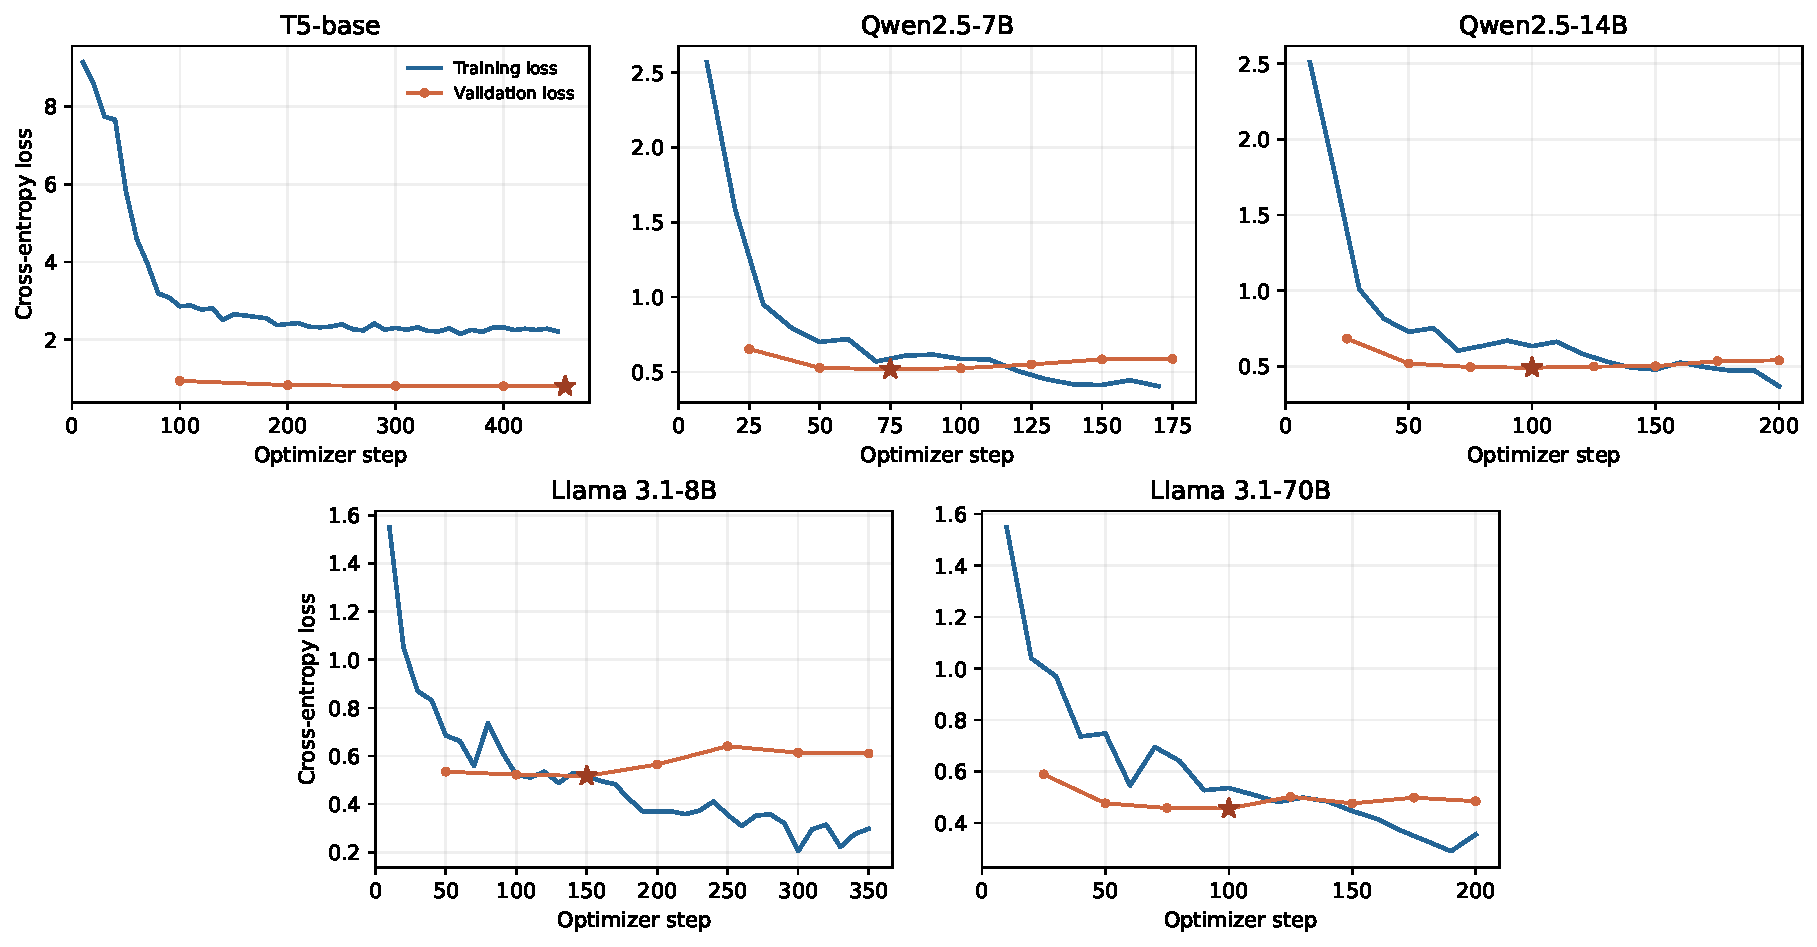
\includegraphics[width=\textwidth]{plots/training_loss_prompt_cleaned.pdf}
\captionof{figure}{Training and validation loss across five models. Stars indicate the selected checkpoints with minimum recorded validation loss. Loss values are not directly comparable across architectures.}
\label{fig:training_loss_prompt_cleaned}
\end{center}

% \subsection{Effectiveness of Urban-Science Instruction Tuning}
% \label{sec:instruction_tuning_effectiveness}

% To evaluate the effectiveness of the proposed instruction corpus, we ask whether dataset-grounded fine-tuning improves urban-data task performance over the corresponding base models (RQ1). We examine this question through matched comparisons of each backbone before and after domain-specific fine-tuning on the same in-domain test partition of held-out resolved source-fact groups. Here, ``base'' denotes the checkpoint before our urban-science training; the Qwen2.5 and Llama 3.1 backbones already have general instruction tuning. Each model is evaluated on 667 multiple-choice and 531 short-answer records, 2,396 positive--negative candidate-verification instances, and 760 structure-preserving paraphrase instances. Answers and explanations are scored separately, yielding 5,552 evaluation rows per checkpoint. These rows share underlying records and concepts and therefore do not constitute 5,552 independent test questions.

% Table~\ref{tab:instruction_tuning_effectiveness} summarizes the matched comparisons. We distinguish normalized answer selection, which accepts recoverable option labels or option text, from strict correctness, which additionally requires an evaluator-accepted answer format. Because accepted formats include a standalone option label, strict correctness does not establish compliance with the complete requested answer-and-explanation schema. Verification is assessed using verdict accuracy and paired consistency across the positive and negative candidates associated with each record. For generation, lexical and semantic scores are interpreted alongside the extraction and preservation checks rather than treated as direct measures of factual correctness.

% \begin{table}[htbp]
% \centering
% \small
% \setlength{\tabcolsep}{5pt}
% \caption{In-domain performance before and after urban-science instruction tuning. MC is normalized multiple-choice accuracy; SA R-L is short-answer ROUGE-L; Verif. is verdict accuracy; Paired is verification paired consistency; Para. is paraphrase BERTScore F1. MC, Verif., and Paired are percentages. All comparisons use the same test records within each task.}
% \label{tab:instruction_tuning_effectiveness}
% \begin{tabular}{llrrrrr}
% \toprule
% Model & Checkpoint & MC & SA R-L & Verif. & Paired & Para. \\
% \midrule
% T5-base & Base & 1.20 & 0.126 & 0.00 & 0.00 & 0.811 \\
% T5-base & Tuned & 63.42 & 0.479 & 54.80 & 12.60 & 0.922 \\
% Qwen2.5-7B & Base & 87.71 & 0.230 & 98.79 & 96.08 & 0.901 \\
% Qwen2.5-7B & Tuned & 100.00 & 0.574 & 98.50 & 96.99 & 0.956 \\
% Qwen2.5-14B & Base & 87.41 & 0.195 & 99.04 & 95.58 & 0.938 \\
% Qwen2.5-14B & Tuned & 100.00 & 0.610 & 99.04 & 98.00 & 0.955 \\
% Llama 3.1-8B & Base & 100.00 & 0.207 & 89.19 & 78.38 & 0.912 \\
% Llama 3.1-8B & Tuned & 100.00 & 0.578 & 99.96 & 99.92 & 0.957 \\
% Llama 3.1-70B & Base & 100.00 & 0.496 & 98.16 & 96.33 & 0.895 \\
% Llama 3.1-70B & Tuned & 100.00 & 0.623 & 98.54 & 97.08 & 0.958 \\
% \bottomrule
% \end{tabular}
% \end{table}

% \paragraph{Answer selection and accepted-answer-format compliance.}
% Fine-tuning brings normalized multiple-choice accuracy to 100\% for all four decoder-only models. Qwen2.5-7B improves from 87.71\% to 100\%, and Qwen2.5-14B from 87.41\% to 100\%, whereas both Llama models already achieve 100\% under normalized scoring before domain-specific training. T5-base improves from 1.20\% to 63.42\%. All five base checkpoints score 0\% under strict multiple-choice scoring, while fine-tuned strict accuracy equals normalized accuracy and accepted-answer-format compliance reaches 100\%. Thus, for the Llama models, the measured multiple-choice benefit is compliance with an evaluator-accepted answer format, with no increase in recoverable answer accuracy. This result alone does not demonstrate that every response includes the requested explanation. The Qwen and T5 results additionally show improved answer selection under the same parser.

% \paragraph{Short answers and explanations.}
% Short-answer ROUGE-L increases for every backbone, from 0.126--0.496 before tuning to 0.479--0.623 after tuning. Fine-tuned exact match ranges from 17.70\% for T5-base to 22.03\% for Qwen2.5-14B. These measures indicate closer agreement with the concise reference answers after tuning, although exact match can reject valid alternative wording. Semantic scores do not improve uniformly: short-answer BERTScore F1 increases from 0.818 to 0.879 for T5-base but decreases slightly for the decoder-only checkpoints. Closer lexical agreement is therefore accompanied by mixed changes in semantic similarity.

% Explanation extraction changes markedly after tuning. The evaluator extracts no separately marked short-answer explanations from any base checkpoint. After fine-tuning, extraction succeeds for all Qwen2.5-7B, Qwen2.5-14B, and Llama 3.1-8B/70B records and all but one T5-base record. Fine-tuned short-answer explanation BERTScores range from 0.889 to 0.900 across the five reported checkpoints. Because base outputs can contain explanatory content outside the expected field markers, this contrast demonstrates improved availability of structured explanations; it does not establish that explanatory reasoning was entirely absent before tuning.

% \paragraph{Candidate verification.}
% Among the decoder-only models, verification gains are largest for Llama 3.1-8B, whose verdict accuracy increases from 89.19\% to 99.96\% and paired consistency from 78.38\% to 99.92\%. Changes are smaller for Llama 3.1-70B (98.16\% to 98.54\% verdict accuracy) and Qwen2.5-14B, whose base verdict accuracies already exceed 98\%. Fine-tuned Qwen2.5-7B shows a small decrease in verdict accuracy, from 98.79\% to 98.50\%, despite an increase in paired consistency from 96.08\% to 96.99\%. Fine-tuned T5-base improves from entirely unparseable base verdicts to 54.80\% accuracy, but its paired consistency remains only 12.60\%. Producing the expected verification fields is insufficient to guarantee reliable discrimination of supported and unsupported candidates.

% \paragraph{Structure-preserving paraphrase.}
% Fine-tuned automated answer preservation is 100\% for both Qwen and both Llama checkpoints but 94.74\% for T5-base; required-field presence remains 100\% for all five. The 40 T5-base preservation failures descend from one held-out Level~3 urban-flow short-answer seed and reflect an altered answer phrase. Before tuning, answer preservation ranges from 0\% to 64.47\%, while field presence remains substantially lower than after tuning. Paraphrase BERTScore increases for every model, reaching 0.922 for T5-base and 0.955--0.958 for the decoder-only models. These results support improved reproduction of the requested structure, but field presence checks only required labels and answer preservation checks a normalized answer string; neither establishes that every explanatory detail survives a rewrite.

% \paragraph{Effectiveness of instruction tuning.}
% The matched results show that urban-science instruction tuning improves task adaptation, particularly accepted output formatting, short-answer reference overlap, and paraphrase preservation. Improvements in answer selection and verification depend on the starting checkpoint, and some metrics remain unchanged or decline. The evidence consequently supports gains in executing the benchmark's grounded instruction tasks, with a substantial contribution from learning the response schema, rather than a uniform improvement in every aspect of urban reasoning. The qualitative audit further motivates separating genuine answer errors from omissions, alternative wording, and scoring artifacts when interpreting these gains.


% \subsection{Effectiveness of Urban-Science Instruction Tuning}
% \label{sec:instruction_tuning_effectiveness}

% To assess whether dataset-grounded fine-tuning improves urban-data task performance (RQ1), we compare each backbone before and after adaptation on the same held-out primary-source concept groups. The evaluation includes 667 multiple-choice, 531 short-answer, 2,396 candidate-verification, and 760 paraphrase instances per checkpoint. Separately scored answers and explanations yield 5,552 evaluation rows, which are not independent source concepts. Table~\ref{tab:instruction_tuning_effectiveness} summarizes the paired results.


% \begin{table}[htbp]
% \centering
% \small
% \setlength{\tabcolsep}{5pt}
% \caption{In-domain performance before and after instruction tuning. MC: normalized multiple-choice accuracy; SA R-L: short-answer ROUGE-L; Verif.: verdict accuracy; Paired: verification paired consistency; Para.: paraphrase BERTScore F1. MC, Verif., and Paired are reported as percentages.}
% \label{tab:instruction_tuning_effectiveness}
% \begin{tabular}{llrrrrr}
% \toprule
% Model & Checkpoint & MC & SA R-L & Verif. & Paired & Para. \\
% \midrule
% T5-base & Base & 1.20 & 0.126 & 0.00 & 0.00 & 0.811 \\
% T5-base & Tuned & 63.42 & 0.479 & 54.80 & 12.60 & 0.922 \\
% Qwen2.5-7B & Base & 87.71 & 0.230 & 98.79 & 96.08 & 0.901 \\
% Qwen2.5-7B & Tuned & 100.00 & 0.574 & 98.50 & 96.99 & 0.956 \\
% Qwen2.5-14B & Base & 87.41 & 0.195 & 99.04 & 95.58 & 0.938 \\
% Qwen2.5-14B & Tuned & 100.00 & 0.610 & 99.04 & 98.00 & 0.955 \\
% Llama 3.1-8B & Base & 100.00 & 0.207 & 89.19 & 78.38 & 0.912 \\
% Llama 3.1-8B & Tuned & 100.00 & 0.578 & 99.96 & 99.92 & 0.957 \\
% Llama 3.1-70B & Base & 100.00 & 0.496 & 98.16 & 96.33 & 0.895 \\
% Llama 3.1-70B & Tuned & 100.00 & 0.623 & 98.54 & 97.08 & 0.958 \\
% \bottomrule
% \end{tabular}
% \end{table}

% \paragraph{Answer selection and format compliance.}
% After fine-tuning, all four decoder-only models reach 100\% normalized multiple-choice accuracy. Qwen2.5-7B and 14B improve from 87.71\% and 87.41\%, respectively, whereas both Llama models already achieve 100\% before adaptation. T5-base improves from 1.20\% to 63.42\%. All base checkpoints score 0\% under strict accuracy, while fine-tuned strict accuracy matches normalized accuracy and accepted-answer-format compliance reaches 100\%. However, strict scoring accepts standalone option labels, so these gains do not establish complete answer-and-explanation schema compliance. For Llama, the observed multiple-choice improvement therefore reflects accepted formatting rather than better answer selection.

% \paragraph{Short answers and explanations.}
% Short-answer ROUGE-L improves for every model, from 0.126--0.496 before tuning to 0.479--0.623 afterward, while fine-tuned exact match ranges from 17.70\% to 22.03\%. Semantic improvements are less consistent: T5-base short-answer BERTScore increases from 0.818 to 0.879, whereas decoder-only scores decline slightly. Explanation extraction also improves substantially. No separately marked short-answer explanations are extracted from base checkpoints, whereas extraction succeeds for every fine-tuned decoder-only response and all but one T5-base response. Fine-tuned explanation BERTScores range from 0.889 to 0.900. These findings indicate improved reference alignment and structured explanation availability, not necessarily the acquisition of additional explanatory knowledge.

% \paragraph{Candidate verification.}
% Llama 3.1-8B shows the largest decoder-only improvement, with verdict accuracy increasing from 89.19\% to 99.96\% and paired consistency from 78.38\% to 99.92\%. Other models show smaller or mixed changes: Qwen2.5-14B maintains 99.04\% verdict accuracy, while Qwen2.5-7B decreases slightly from 98.79\% to 98.50\% despite improved paired consistency. T5-base reaches 54.80\% verdict accuracy after tuning, but only 12.60\% paired consistency. Thus, successful output formatting does not guarantee reliable discrimination between supported and unsupported candidates.

% \paragraph{Structure-preserving paraphrase.}
% Fine-tuned answer preservation reaches 100\% for all decoder-only models and 94.74\% for T5-base, with 100\% required-field presence across all five. The 40 T5-base failures originate from one held-out Level~3 urban-flow seed. Paraphrase BERTScore improves for every model, reaching 0.922 for T5-base and 0.955--0.958 for decoder-only models. Nevertheless, automated field and answer checks do not establish complete semantic preservation.

% \paragraph{Overall effectiveness.}
% Fine-tuning consistently improves accepted output formatting, short-answer reference overlap, and automated paraphrase preservation. Answer-selection and verification gains vary with the starting checkpoint. The results therefore support improved execution of source-grounded instruction tasks, while distinguishing schema learning from broader gains in factual understanding.



\subsection{Effectiveness of Urban-Science Instruction Tuning}
\label{sec:instruction_tuning_effectiveness}

To address RQ1, we compare base and fine-tuned checkpoints on the same held-out primary-source concept groups. Each checkpoint is evaluated on 667 multiple-choice, 531 short-answer, 2,396 verification, and 760 paraphrase instances. Separate answer and explanation scores yield 5,552 evaluation rows, not independent concepts. Table~\ref{tab:instruction_tuning_effectiveness} summarizes the results.

\begin{table}[htbp]
\centering
\small
\setlength{\tabcolsep}{5pt}
\caption{In-domain performance before and after instruction tuning. MC: normalized multiple-choice accuracy; SA R-L: short-answer ROUGE-L; Verif.: verdict accuracy; Paired: verification paired consistency; Para.: paraphrase BERTScore F1. MC, Verif., and Paired are percentages.}
\label{tab:instruction_tuning_effectiveness}
\begin{tabular}{llrrrrr}
\toprule
Model & Checkpoint & MC & SA R-L & Verif. & Paired & Para. \\
\midrule
T5-base & Base & 1.20 & 0.126 & 0.00 & 0.00 & 0.811 \\
T5-base & Tuned & 63.42 & 0.479 & 54.80 & 12.60 & 0.922 \\
Qwen2.5-7B & Base & 87.71 & 0.230 & 98.79 & 96.08 & 0.901 \\
Qwen2.5-7B & Tuned & 100.00 & 0.574 & 98.50 & 96.99 & 0.956 \\
Qwen2.5-14B & Base & 87.41 & 0.195 & 99.04 & 95.58 & 0.938 \\
Qwen2.5-14B & Tuned & 100.00 & 0.610 & 99.04 & 98.00 & 0.955 \\
Llama 3.1-8B & Base & 100.00 & 0.207 & 89.19 & 78.38 & 0.912 \\
Llama 3.1-8B & Tuned & 100.00 & 0.578 & 99.96 & 99.92 & 0.957 \\
Llama 3.1-70B & Base & 100.00 & 0.496 & 98.16 & 96.33 & 0.895 \\
Llama 3.1-70B & Tuned & 100.00 & 0.623 & 98.54 & 97.08 & 0.958 \\
\bottomrule
\end{tabular}
\end{table}

\paragraph{Answer selection and verification.}
After tuning, all decoder-only models achieve 100\% normalized multiple-choice accuracy; both Llama models already reached this level before tuning, whereas T5-base improves from 1.20\% to 63.42\%. Strict accuracy rises from zero across all base checkpoints to match normalized accuracy after tuning, with 100\% accepted-answer-format compliance. However, standalone labels satisfy strict scoring, so full schema compliance is not established. Verification gains vary: Llama 3.1-8B improves to 99.96\% verdict accuracy and 99.92\% paired consistency, whereas Qwen changes are small or mixed. T5-base reaches 54.80\% verdict accuracy but only 12.60\% paired consistency, indicating that formatting compliance does not ensure reliable verification.

\paragraph{Short answers and paraphrases.}
Short-answer ROUGE-L improves across all models to 0.479--0.623, although exact match remains at 17.70--22.03\%. T5-base short-answer BERTScore increases from 0.818 to 0.879, while decoder-only scores decline slightly. Base checkpoints yield no separately extracted short-answer explanations; after tuning, extraction succeeds for all decoder-only responses and all but one T5-base response, with explanation BERTScores of 0.889--0.900. Paraphrase BERTScore increases to 0.922--0.958, with 100\% answer preservation for decoder-only models and 94.74\% for T5-base. All models retain required fields; T5-base's 40 preservation failures originate from one Level~3 urban-flow seed. Neither reference similarity nor automated preservation establishes factual or semantic equivalence.

Overall, instruction tuning improves output formatting, short-answer reference alignment, and paraphrase preservation, while gains in answer selection and verification depend on the base checkpoint.

% \subsection{Comparison Across Model Families and Scales}
% \label{sec:model_family_scale}

% The different adaptation gains observed in Section~\ref{sec:instruction_tuning_effectiveness} raise a further question: how do the benefits and limitations of urban-science instruction tuning vary across model families and scales (RQ2)? To examine whether these patterns extend across backbones, we compare the two sizes within each decoder-only family and include T5-base as a smaller encoder--decoder reference. These comparisons describe the evaluated configurations: model size, pretraining, prior instruction tuning, and adaptation settings are not independently controlled, so differences cannot be attributed to architecture or parameter count alone.

% \begin{table}[htbp]
% \centering
% \small
% \setlength{\tabcolsep}{5pt}
% \caption{Fine-tuned in-domain generation performance. SA EM: normalized exact match (\%); SA R-L: ROUGE-L; SA NLI: mean entailment score; MC/SA Exp.: explanation BERTScore F1. Semantic metrics do not represent human-validated correctness.}
% \label{tab:model_family_generation}
% \begin{tabular}{lrrrrr}
% \toprule
% Model & SA EM & SA R-L & SA NLI & MC Exp. & SA Exp. \\
% \midrule
% T5-base & 17.70 & 0.479 & 0.543 & 0.903 & 0.889 \\
% Qwen2.5-7B & 20.34 & 0.574 & 0.607 & 0.923 & 0.898 \\
% Qwen2.5-14B & 22.03 & 0.610 & 0.551 & 0.917 & 0.896 \\
% Llama 3.1-8B & 19.40 & 0.578 & 0.619 & 0.917 & 0.900 \\
% Llama 3.1-70B & 19.77 & 0.623 & 0.699 & 0.917 & 0.899 \\
% \bottomrule
% \end{tabular}
% \end{table}

% \paragraph{Llama 3.1: stronger short-answer alignment at larger scale.}
% Both fine-tuned Llama models reach 100\% normalized and strict multiple-choice accuracy, leaving no observed separation on answer selection in this test partition. Differences emerge in short-answer generation: 70B achieves higher ROUGE-L than 8B (0.623 versus 0.578), slightly higher exact match (19.77\% versus 19.40\%), and higher mean NLI entailment (0.699 versus 0.619). Explanation BERTScores remain close, at about 0.917 for multiple-choice explanations and 0.899--0.900 for short-answer explanations. The 70B checkpoint therefore achieves stronger short-answer reference alignment on these measures, while explanation similarity remains comparable.

% Verification reverses this ordering. Fine-tuned Llama 3.1-8B achieves 99.96\% verdict accuracy and 99.92\% paired consistency, compared with 98.54\% and 97.08\% for 70B. The smaller model also has more room to improve from its base verification accuracy of 89.19\%, whereas the larger model starts at 98.16\%. These results distinguish adaptation gain from final performance and show that the larger checkpoint is not uniformly stronger in-domain.

% \paragraph{Qwen2.5: scale-dependent trade-offs between reference overlap and semantic scores.}
% Both Qwen models reach 100\% in-domain multiple-choice accuracy after tuning. Qwen2.5-14B retains the highest short-answer exact match among the five reported checkpoints (22.03\%) and exceeds Qwen2.5-7B in short-answer ROUGE-L (0.610 versus 0.574). It also has higher verification accuracy (99.04\% versus 98.50\%) and paired consistency (98.00\% versus 96.99\%). The 7B model, however, has a higher mean short-answer entailment score (0.607 versus 0.551) and higher multiple-choice explanation BERTScore (0.923 versus 0.917). Closer reference wording at 14B therefore does not imply dominance under every semantic measure.

% \paragraph{T5-base: successful format adaptation with residual discrimination errors.}
% Fine-tuned T5-base improves substantially from its weak base performance, but its fine-tuned multiple-choice accuracy of 63.42\% and verification accuracy of 54.80\% remain below those of the decoder-only models. Its 12.60\% paired verification consistency is particularly informative: even with 100\% verification format compliance, it often fails to correctly handle both candidates for the same underlying record. At the same time, its short-answer BERTScore reaches 0.879, close to the decoder-only range, despite lower short-answer ROUGE-L and exact match. Similarity alone therefore provides an incomplete account of its task performance.

% T5-base reaches 100\% required-field presence in the in-domain paraphrase task but 94.74\% answer preservation. This concentration of preservation failures in one Level~3 seed illustrates why high semantic similarity and correct formatting should not be treated as complete preservation. Its limitations in answer selection and verification should not be generalized to every structured task, nor treated as evidence that encoder--decoder architectures inherently cannot perform constrained prediction.

% \paragraph{Differences across models.}
% The five backbones exhibit different task profiles rather than a single ordering by model size. Fine-tuned Llama 3.1-70B leads the reported short-answer ROUGE-L and mean entailment scores, Qwen2.5-14B leads short-answer exact match, Llama 3.1-8B leads in-domain verification accuracy and paired consistency, and Qwen2.5-7B leads multiple-choice explanation BERTScore. T5-base demonstrates substantial adaptation while retaining larger answer-selection and verification limitations. All five use the same training corpus, but these cross-model rankings remain descriptive because pretraining, scale, and the 70B quantization source differ. Small differences in semantic scores should be interpreted cautiously because statistical significance has not been established.


\subsection{Comparison Across Model Families and Scales}
\label{sec:model_family_scale}

To address RQ2, we compare fine-tuned performance across the two sizes of each decoder-only family, using T5-base as an encoder--decoder reference. These comparisons are descriptive: architecture, parameter count, pretraining, prior instruction tuning, and adaptation settings are not independently controlled.

\begin{table}[htbp]
\centering
\small
\setlength{\tabcolsep}{5pt}
\caption{Fine-tuned in-domain generation performance. SA EM: normalized exact match (\%); SA R-L: ROUGE-L; SA NLI: mean entailment score; MC/SA Exp.: explanation BERTScore F1. Semantic metrics do not represent human-validated correctness.}
\label{tab:model_family_generation}
\begin{tabular}{lrrrrr}
\toprule
Model & SA EM & SA R-L & SA NLI & MC Exp. & SA Exp. \\
\midrule
T5-base & 17.70 & 0.479 & 0.543 & 0.903 & 0.889 \\
Qwen2.5-7B & 20.34 & 0.574 & 0.607 & 0.923 & 0.898 \\
Qwen2.5-14B & 22.03 & 0.610 & 0.551 & 0.917 & 0.896 \\
Llama 3.1-8B & 19.40 & 0.578 & 0.619 & 0.917 & 0.900 \\
Llama 3.1-70B & 19.77 & 0.623 & 0.699 & 0.917 & 0.899 \\
\bottomrule
\end{tabular}
\end{table}

\paragraph{Llama 3.1: task-dependent scale effects.}
Both fine-tuned Llama models achieve 100\% in-domain multiple-choice accuracy. The 70B model shows stronger short-answer alignment, with higher ROUGE-L (0.623 versus 0.578) and mean NLI entailment (0.699 versus 0.619), while explanation similarity remains comparable. However, 8B achieves higher verification accuracy (99.96\% versus 98.54\%) and paired consistency (99.92\% versus 97.08\%). The larger model is therefore not uniformly stronger, and its smaller verification gains partly reflect its higher base accuracy (98.16\% versus 89.19\%).

\paragraph{Qwen2.5: lexical and semantic trade-offs.}
Both fine-tuned Qwen models achieve 100\% multiple-choice accuracy. Qwen2.5-14B leads in short-answer exact match (22.03\%), ROUGE-L (0.610 versus 0.574), verification accuracy (99.04\% versus 98.50\%), and paired consistency (98.00\% versus 96.99\%). However, 7B achieves higher mean NLI entailment (0.607 versus 0.551) and multiple-choice explanation BERTScore (0.923 versus 0.917). Greater reference overlap at 14B thus does not translate into uniformly higher semantic scores.

\paragraph{T5-base and cross-model differences.}
T5-base improves substantially after tuning but remains weaker in answer selection (63.42\% multiple-choice accuracy) and verification (54.80\% accuracy; 12.60\% paired consistency), despite 100\% verification format compliance. Its relatively high short-answer BERTScore (0.879) further illustrates that semantic similarity does not guarantee task correctness. In paraphrasing, required-field presence reaches 100\%, but answer preservation remains at 94.74\%, with failures concentrated in one Level~3 seed.

Overall, the models exhibit task-specific strengths rather than a consistent ranking by scale: Llama 3.1-70B leads short-answer ROUGE-L and NLI, Qwen2.5-14B leads exact match, Llama 3.1-8B leads verification, and Qwen2.5-7B leads multiple-choice explanation similarity. These rankings should not be interpreted as isolated architecture or scaling effects, particularly given differences in pretraining and quantization provenance. Small semantic-score differences also lack established statistical significance.


% \subsection{Performance Across Tasks and Reasoning Levels}
% \label{sec:task_difficulty_results}

% Overall model comparisons can conceal differences in the demands of individual tasks. To identify where the fine-tuned models perform reliably and where challenges remain, we ask how performance varies across task types and reasoning difficulty levels (RQ3). We examine the in-domain results at the three levels defined in Section~3: direct dataset comprehension, multi-attribute reasoning, and cross-dimensional interpretation. Answer generation, candidate verification, and structure-preserving paraphrase evaluate different behaviors, even when they originate from the same canonical record. We compare models within each task and level to distinguish these behaviors.

% \paragraph{Test coverage and interpretation.}
% Table~\ref{tab:task_level_coverage} reports the number of evaluated instances per model. Level~1 dominates the test partition, and no Level~3 multiple-choice records are present. Moreover, the 408 Level~1 short-answer records descend from eight seeds across all five primary sources, whereas the 41 Level~2 short-answer records descend from one TLC seed and the 82 Level~3 records from two urban-flow seeds. The resolved source-fact group split keeps seeds and descendants from the same group within one partition, but it produces uneven source and seed coverage across levels. Consequently, differences below describe these held-out subsets; they do not isolate the causal effect of reasoning difficulty from source content or augmentation patterns.

% \begin{table}[htbp]
% \centering
% \small
% \caption{In-domain test instances by task and reasoning level. Counts represent evaluation instances, not independent concepts.}
% \label{tab:task_level_coverage}
% \begin{tabular}{lrrrr}
% \toprule
% Task & Level 1 & Level 2 & Level 3 & Total \\
% \midrule
% Multiple-choice answer & 606 & 61 & 0 & 667 \\
% Short answer & 408 & 41 & 82 & 531 \\
% Candidate verification & 2,028 & 204 & 164 & 2,396 \\
% Structure-preserving paraphrase & 620 & 60 & 80 & 760 \\
% \bottomrule
% \end{tabular}
% \end{table}

% \paragraph{Answer selection versus short-answer generation.}
% The four decoder-only models achieve 100\% normalized and strict multiple-choice accuracy at both observed levels. This ceiling limits the ability of multiple-choice accuracy to distinguish their performance on these subsets. Fine-tuned T5-base achieves 63.04\% at Level~1 and 67.21\% at Level~2; the assigned reasoning level does not by itself determine measured accuracy when test content differs.

% Short-answer results provide greater differentiation (Table~\ref{tab:task_level_performance}). ROUGE-L decreases from Level~1 to Level~3 for every model: the Level~1 range of 0.541--0.707 falls to 0.192--0.234 at Level~3. Level~2 performance is intermediate, although Llama 3.1-70B retains higher overlap (0.627) than the other backbones (0.402--0.495). All five models have zero short-answer exact match at Levels~2 and~3, compared with 23.04--28.68\% at Level~1. This means none exactly reproduces the normalized higher-level references; it does not establish that all those answers are factually incorrect.

% \begin{table}[htbp]
% \centering
% \small
% \setlength{\tabcolsep}{5pt}
% \caption{Fine-tuned performance by reasoning level. Task-specific denominators are reported in Table~\ref{tab:task_level_coverage}.}
% \label{tab:task_level_performance}
% \begin{tabular}{lrrrrrr}
% \toprule
%  & \multicolumn{3}{c}{Short-answer ROUGE-L} & \multicolumn{3}{c}{Verification accuracy (\%)} \\
% \cmidrule(lr){2-4}\cmidrule(lr){5-7}
% Model & L1 & L2 & L3 & L1 & L2 & L3 \\
% \midrule
% T5-base & 0.541 & 0.445 & 0.192 & 55.13 & 50.00 & 56.71 \\
% Qwen2.5-7B & 0.659 & 0.495 & 0.193 & 99.56 & 99.02 & 84.76 \\
% Qwen2.5-14B & 0.707 & 0.417 & 0.221 & 99.26 & 99.51 & 95.73 \\
% Llama 3.1-8B & 0.672 & 0.402 & 0.200 & 99.95 & 100.00 & 100.00 \\
% Llama 3.1-70B & 0.701 & 0.627 & 0.234 & 99.31 & 99.02 & 88.41 \\
% \bottomrule
% \end{tabular}
% \end{table}

% \paragraph{Semantic alignment and explanatory content.}
% Semantic metrics qualify the sharp lexical decline. Level~3 short-answer BERTScores remain between 0.854 and 0.865, despite the low ROUGE-L values and zero exact match. Mean short-answer NLI scores are highest at Level~2 for every model, ranging from 0.700 to 0.827, rather than decreasing monotonically with assigned difficulty. Short-answer explanation BERTScores are lower at Level~3 than at either preceding level for all five models, with Level~3 values ranging from 0.863 to 0.877. These measures indicate reduced reference alignment in the Level~3 subset while leaving the distinction between valid reformulation and missing information unresolved. The exploratory qualitative audit identifies both behaviors but does not establish a level-specific error rate.

% \paragraph{Candidate verification.}
% Verification shows a different pattern from generation. At Level~3, Qwen2.5-7B and Llama 3.1-70B achieve 84.76\% and 88.41\% verdict accuracy, respectively, compared with approximately 99\% at the preceding levels. Fine-tuned Qwen2.5-14B decreases less sharply to 95.73\%, while Llama 3.1-8B correctly classifies all 164 Level~3 candidates. T5-base remains between 50.00\% and 56.71\% across levels, near the 50\% constant-verdict baseline for this balanced task. The same source questions can therefore yield weak reference overlap in free generation and strong performance when a candidate is supplied. These tasks probe complementary response behaviors.

% \paragraph{Structure-preserving paraphrase.}
% Both Qwen and both Llama models retain 100\% automated answer preservation and required-field presence at each level. Fine-tuned T5-base retains all required fields but preserves the normalized answer in only 50\% of Level~3 paraphrases: 40 descendants of one urban-flow seed alter the answer phrase. Paraphrase BERTScore generally falls from Level~1 to Level~3, while the T5-base values are 0.922 and 0.921 at those levels. Unlike answer generation, this task supplies a completed instruction to rewrite. Strong preservation scores therefore demonstrate a different behavior from independently producing an answer and explanation, and even saturated structural checks cannot establish complete factual preservation.

% \paragraph{Implications of task and level differences.}
% Task type and test-subset composition materially affect the observed results. Multiple-choice selection and automated paraphrase preservation reach ceilings for the decoder-only models, whereas open-ended answers and explanations expose greater variation and lower reference alignment on Level~3 examples. Verification difficulty is model-dependent rather than uniformly increasing across levels. The findings support evaluating selection, generation, discrimination, and preservation separately. Given the limited and uneven seed coverage, they provide descriptive evidence about the tested reasoning levels rather than a general ranking of intrinsic task difficulty.


\subsection{Performance Across Tasks and Reasoning Levels}
\label{sec:task_difficulty_results}

To address RQ3, we compare fine-tuned in-domain performance across three reasoning levels and three task views: answer generation, candidate verification, and structure-preserving paraphrase.

\paragraph{Test coverage.}
Level~1 dominates the test partition, with no Level~3 multiple-choice records (Table~\ref{tab:task_level_coverage}). Level~1 short answers derive from eight seeds across five sources, whereas Levels~2 and~3 derive from one TLC seed and two urban-flow seeds, respectively. Despite concept-group partitioning, uneven source and seed coverage prevents attributing performance differences solely to reasoning difficulty.

\begin{table}[htbp]
\centering
\small
\caption{In-domain test instances by task and reasoning level. Counts represent evaluation instances, not independent concepts.}
\label{tab:task_level_coverage}
\begin{tabular}{lrrrr}
\toprule
Task & Level 1 & Level 2 & Level 3 & Total \\
\midrule
Multiple-choice answer & 606 & 61 & 0 & 667 \\
Short answer & 408 & 41 & 82 & 531 \\
Candidate verification & 2,028 & 204 & 164 & 2,396 \\
Structure-preserving paraphrase & 620 & 60 & 80 & 760 \\
\bottomrule
\end{tabular}
\end{table}

\paragraph{Answer generation.}
All four decoder-only models achieve 100\% normalized and strict multiple-choice accuracy at both observed levels; T5-base reaches 63.04\% at Level~1 and 67.21\% at Level~2.

Short-answer ROUGE-L declines across levels for every model, from 0.541--0.707 at Level~1 to 0.192--0.234 at Level~3 (Table~\ref{tab:task_level_performance}). Exact match similarly falls from 23.04--28.68\% to zero, without necessarily indicating factual errors. Semantic metrics are less consistent: Level~3 BERTScores remain at 0.854--0.865, NLI entailment peaks at Level~2 (0.700--0.827), and explanation BERTScores decline to 0.863--0.877 at Level~3. These differences suggest reduced reference alignment rather than establishing incorrectness, as the qualitative audit identifies both valid reformulations and substantive errors.

\begin{table}[htbp]
\centering
\small
\setlength{\tabcolsep}{5pt}
\caption{Fine-tuned performance by reasoning level. Task-specific denominators are reported in Table~\ref{tab:task_level_coverage}.}
\label{tab:task_level_performance}
\begin{tabular}{lrrrrrr}
\toprule
 & \multicolumn{3}{c}{Short-answer ROUGE-L} & \multicolumn{3}{c}{Verification accuracy (\%)} \\
\cmidrule(lr){2-4}\cmidrule(lr){5-7}
Model & L1 & L2 & L3 & L1 & L2 & L3 \\
\midrule
T5-base & 0.541 & 0.445 & 0.192 & 55.13 & 50.00 & 56.71 \\
Qwen2.5-7B & 0.659 & 0.495 & 0.193 & 99.56 & 99.02 & 84.76 \\
Qwen2.5-14B & 0.707 & 0.417 & 0.221 & 99.26 & 99.51 & 95.73 \\
Llama 3.1-8B & 0.672 & 0.402 & 0.200 & 99.95 & 100.00 & 100.00 \\
Llama 3.1-70B & 0.701 & 0.627 & 0.234 & 99.31 & 99.02 & 88.41 \\
\bottomrule
\end{tabular}
\end{table}

\paragraph{Candidate verification.}
Verification does not decline uniformly with reasoning level. At Level~3, Qwen2.5-7B and Llama 3.1-70B fall to 84.76\% and 88.41\%, while Llama 3.1-8B achieves 100\%. T5-base remains near the balanced-task baseline (50.00--56.71\%). This contrasts with consistently declining short-answer ROUGE-L, indicating distinct generation and discrimination behaviors.

\paragraph{Structure-preserving paraphrase.}
All decoder-only models achieve 100\% automated answer and field preservation across levels. T5-base retains required fields but preserves only 50\% of Level~3 answers, with 40 failures from one urban-flow seed. Paraphrase BERTScore generally declines with level, except for T5-base (0.922 versus 0.921 at Levels~1 and~3). Because the task supplies completed instructions, preservation does not establish independent answering ability or complete factual equivalence.

\paragraph{Implications.}
Multiple-choice and paraphrase preservation approach ceiling performance, whereas open-ended generation shows greater variation and weaker Level~3 reference alignment. Verification varies by model rather than following a consistent difficulty hierarchy. Given uneven independent seed coverage, these comparisons remain descriptive.


% \subsection{Generalization Across Regions and Datasets}
% \label{sec:generalization_results}

% To evaluate whether the learned task behaviors extend beyond the primary urban-data sources, we ask how well instruction tuning generalizes to unseen regional and dataset contexts (RQ4). We examine two complementary settings: controlled variants from the geographically held-out French and Japanese sources, and the independent benchmark of ten previously unseen datasets. Each comparison uses the same test prompts for the base and fine-tuned checkpoints without further adaptation. Because the prompts supply the relevant source context, these experiments evaluate transfer in interpreting unfamiliar dataset information, rather than unaided recall of regional knowledge.

% \paragraph{Transfer to France and Japan.}
% The geographically held-out evaluation contains 2,428 multiple-choice and 1,738 short-answer records, 8,332 verification instances, and 2,420 paraphrase instances. Table~\ref{tab:regional_transfer} shows that instruction tuning improves normalized multiple-choice accuracy for every backbone. The decoder-only models reach 99.18--99.92\%, compared with base accuracies of 74.59--95.88\%. Fine-tuned T5-base improves from 5.31\% to 73.68\%. Fine-tuned strict and normalized multiple-choice accuracies coincide, indicating that all responses credited as correct under normalized scoring also satisfy an evaluator-accepted answer format. This does not establish that every response includes the requested explanation.

% \begin{table}[htbp]
% \centering
% \small
% \caption{Base and fine-tuned performance on the held-out France--Japan evaluation. MC is normalized multiple-choice accuracy (\%); SA R-L is short-answer ROUGE-L; Verif. and Paired denote verdict accuracy and paired verification consistency (\%).}
% \label{tab:regional_transfer}
% \begin{tabular}{llrrrr}
% \toprule
% Model & Checkpoint & MC & SA R-L & Verif. & Paired \\
% \midrule
% T5-base & Base & 5.31 & 0.085 & 0.00 & 0.00 \\
% T5-base & Tuned & 73.68 & 0.295 & 54.97 & 14.33 \\
% Qwen2.5-7B & Base & 83.53 & 0.199 & 97.11 & 94.24 \\
% Qwen2.5-7B & Tuned & 99.18 & 0.399 & 99.08 & 98.18 \\
% Qwen2.5-14B & Base & 74.59 & 0.169 & 98.69 & 89.13 \\
% Qwen2.5-14B & Tuned & 99.67 & 0.348 & 99.74 & 98.73 \\
% Llama 3.1-8B & Base & 95.88 & 0.127 & 92.35 & 83.39 \\
% Llama 3.1-8B & Tuned & 99.84 & 0.392 & 98.36 & 92.82 \\
% Llama 3.1-70B & Base & 94.48 & 0.261 & 99.08 & 98.10 \\
% Llama 3.1-70B & Tuned & 99.92 & 0.411 & 99.38 & 98.78 \\
% \bottomrule
% \end{tabular}
% \end{table}

% Verification accuracy also improves for all models relative to their base checkpoints. The four decoder-only models achieve 98.36--99.74\% accuracy and 92.82--98.78\% paired consistency. Fine-tuned T5-base reaches 54.97\% accuracy but only 14.33\% paired consistency, preserving the substantial discrimination limitation observed in-domain. T5-base multiple-choice accuracy is 81.71\% on France and 65.65\% on Japan; the Qwen2.5-7B reaches 100\% and 98.35\%, respectively, and Qwen2.5-14B reaches 100\% and 99.34\%. Averaging T5 scores within each multiple-choice seed and then weighting the seed means equally gives 79.15\% for France and 64.02\% for Japan. This selected-model sensitivity check reduces the influence of unequal descendant counts, although the regional comparison still covers only 33 authored seeds per source across tasks.

% \paragraph{Generation and preservation under regional shift.}
% Short-answer ROUGE-L improves over the base checkpoint for all five models, but the fine-tuned cross-regional values remain below their in-domain counterparts. The decoder-only range falls from 0.574--0.623 in-domain to 0.348--0.411 on France and Japan; T5-base decreases from 0.479 to 0.295. Thus, near-ceiling multiple-choice accuracy does not imply equivalent reference alignment in open-ended responses. These differences involve distinct source and question distributions and should not be attributed exclusively to geography.

% Paraphrase performance transfers less uniformly across models. Fine-tuned T5-base, Qwen2.5-14B, and both Llama models achieve 100\% automated answer and field preservation. Fine-tuned Qwen2.5-7B achieves 97.77\% on both measures, with the same 54 failures among 2,420 regional paraphrases. These failures are descendants of one Japanese question and contain the correct option, B, but replace the required \texttt{EXPLANATION:} label with \texttt{EXPLANIFICATION:}. The field-preservation check rejects this misspelled label. The answer parser also fails to recognize the explanation boundary, causing the extracted answer to include the explanation text and fail normalized answer equality. These cases therefore reflect formatting and parsing failures despite correct option selection. These automated checks do not establish preservation of every factual detail.

% \paragraph{Transfer to ten independent datasets.}
% The broader external benchmark contains 350 authored answer-generation records: 150 multiple-choice and 200 short-answer questions, accompanied by 700 balanced verification instances. Each of the ten datasets contributes 15 multiple-choice questions, 20 short-answer questions, and 70 verification instances. No augmented paraphrase descendants are included. Consequently, the task-level row averages in Table~\ref{tab:external_transfer} also equal the corresponding unweighted dataset-level macro averages.

% \begin{table}[htbp]
% \centering
% \small
% \caption{Performance on the independent ten-dataset benchmark. Metric definitions match Table~\ref{tab:regional_transfer}. Equal task counts per dataset make the reported row averages equal to dataset-macro averages for MC, SA R-L, and verdict accuracy.}
% \label{tab:external_transfer}
% \begin{tabular}{llrrrr}
% \toprule
% Model & Checkpoint & MC & SA R-L & Verif. & Paired \\
% \midrule
% T5-base & Base & 11.33 & 0.037 & 0.00 & 0.00 \\
% T5-base & Tuned & 74.00 & 0.319 & 54.00 & 17.43 \\
% Qwen2.5-7B & Base & 90.00 & 0.246 & 90.86 & 82.00 \\
% Qwen2.5-7B & Tuned & 94.00 & 0.359 & 91.43 & 82.86 \\
% Qwen2.5-14B & Base & 95.33 & 0.199 & 92.43 & 79.14 \\
% Qwen2.5-14B & Tuned & 96.67 & 0.332 & 90.29 & 79.43 \\
% Llama 3.1-8B & Base & 88.67 & 0.167 & 67.43 & 35.43 \\
% Llama 3.1-8B & Tuned & 90.67 & 0.312 & 89.00 & 78.57 \\
% Llama 3.1-70B & Base & 97.33 & 0.311 & 92.00 & 84.86 \\
% Llama 3.1-70B & Tuned & 98.00 & 0.365 & 92.71 & 86.00 \\
% \bottomrule
% \end{tabular}
% \end{table}

% Fine-tuned decoder-only multiple-choice accuracy ranges from 90.67\% to 98.00\%, below the France--Japan results. Fine-tuned Llama 3.1-70B rises from 97.33\% to 98.00\%, one additional correct option among 150 external questions. Short-answer ROUGE-L improves for every backbone, reaching 0.312--0.365 for the decoder-only models and 0.319 for T5-base. These gains demonstrate closer reference alignment on new datasets, but do not establish complete factual correctness of the generated responses.

% Verification provides a clearer indication of the remaining transfer gap. Fine-tuned decoder-only accuracy ranges from 89.00\% to 92.71\%, compared with 98.36--99.74\% on France and Japan. Fine-tuned Qwen2.5-7B rises from 90.86\% at base stage to 91.43\%, while Qwen2.5-14B falls from 92.43\% to 90.29\%. Fine-tuned Llama 3.1-70B reaches the highest external verdict accuracy, 92.71\%, while remaining below its 99.38\% France--Japan result. Fine-tuned T5-base reaches 54.00\%, still near the balanced task's 50\% constant-verdict baseline. The benefits of adaptation therefore extend to new sources but are neither uniform across models nor sufficient to eliminate discrimination errors.

% Dataset-level variation also remains visible. Fine-tuned Llama 3.1-70B multiple-choice accuracy ranges from 80.00\% to 100\% across sources, despite its 98.00\% overall result; each source contains only 15 multiple-choice questions, so a small number of errors produces a sizable percentage change. A leave-one-dataset-out sensitivity analysis places its verification accuracy between 92.22\% and 93.17\%, suggesting that the overall verification result is not driven by a single dataset. These selected-model diagnostics characterize source variation for fine-tuned Llama 3.1-70B without treating related task views as independent observations.

% \paragraph{Scope of generalization.}
% Instruction tuning transfers useful answer-selection, verification, and response-structuring behaviors beyond the primary sources. For the decoder-only models, answer-selection and verification performance is higher on the controlled France--Japan evaluation than on the ten-dataset benchmark, where both source coverage and question content broaden. The results support generalization in context-grounded task execution while identifying persistent limitations in open-ended reference alignment and candidate discrimination. They do not establish unrestricted geographic generalization or professional planning competence, and the controlled regional variants should not be counted as thousands of independent tests of new knowledge.


\subsection{Generalization Across Regions and Datasets}
\label{sec:generalization_results}

To assess transfer beyond the primary sources (RQ4), we evaluate matched base and fine-tuned checkpoints on controlled France--Japan variants and independently authored questions from ten additional datasets. Both settings supply source context, testing interpretation of unseen information rather than unaided factual recall.

\paragraph{Transfer to France and Japan.}
The regional holdout contains 2,428 multiple-choice, 1,738 short-answer, 8,332 verification, and 2,420 paraphrase instances. Fine-tuning improves multiple-choice and verification performance across all models (Table~\ref{tab:regional_transfer}). Decoder-only models achieve 99.18--99.92\% multiple-choice accuracy and 98.36--99.74\% verification accuracy, while T5-base reaches 73.68\% and 54.97\%, respectively. Strict and normalized multiple-choice accuracy coincide after tuning, indicating accepted answer formatting without establishing complete schema compliance. T5-base's paired verification consistency remains low at 14.33\%.

\begin{table}[htbp]
\centering
\small
\caption{Base and fine-tuned performance on the France--Japan held-out evaluation. MC, Verif., and Paired are percentages.}
\label{tab:regional_transfer}
\begin{tabular}{llrrrr}
\toprule
Model & Checkpoint & MC & SA R-L & Verif. & Paired \\
\midrule
T5-base & Base & 5.31 & 0.085 & 0.00 & 0.00 \\
T5-base & Tuned & 73.68 & 0.295 & 54.97 & 14.33 \\
Qwen2.5-7B & Base & 83.53 & 0.199 & 97.11 & 94.24 \\
Qwen2.5-7B & Tuned & 99.18 & 0.399 & 99.08 & 98.18 \\
Qwen2.5-14B & Base & 74.59 & 0.169 & 98.69 & 89.13 \\
Qwen2.5-14B & Tuned & 99.67 & 0.348 & 99.74 & 98.73 \\
Llama 3.1-8B & Base & 95.88 & 0.127 & 92.35 & 83.39 \\
Llama 3.1-8B & Tuned & 99.84 & 0.392 & 98.36 & 92.82 \\
Llama 3.1-70B & Base & 94.48 & 0.261 & 99.08 & 98.10 \\
Llama 3.1-70B & Tuned & 99.92 & 0.411 & 99.38 & 98.78 \\
\bottomrule
\end{tabular}
\end{table}

Country-specific multiple-choice accuracy for T5-base is 81.71\% in France and 65.65\% in Japan, versus seed-weighted accuracies of 79.15\% and 64.02\%. This sensitivity check reduces descendant-count imbalance but cannot overcome limited independent seed coverage. Qwen2.5-7B and Qwen2.5-14B achieve 100\% accuracy in France and 98.35\% and 99.34\%, respectively, in Japan.

\paragraph{Generation and preservation under regional shift.}
Short-answer ROUGE-L improves after tuning but remains below in-domain levels: 0.348--0.411 versus 0.574--0.623 for decoder-only models, and 0.295 versus 0.479 for T5-base. Thus, near-ceiling multiple-choice accuracy does not imply comparable open-ended alignment; source and question distributions also differ.

Automated paraphrase preservation reaches 100\% for four models, but Qwen2.5-7B reaches 97.77\%, with 54 failures from one Japanese question. These responses retain the correct option but use \texttt{EXPLANIFICATION:} instead of \texttt{EXPLANATION:}, disrupting field preservation and answer extraction. Automated preservation does not guarantee complete factual fidelity.

\paragraph{Transfer to ten independent datasets.}
The second benchmark contains 350 independently authored generation records and 700 verification instances, with equal per-source task counts and no paraphrase augmentation (Table~\ref{tab:external_transfer}).

\begin{table}[htbp]
\centering
\small
\caption{Base and fine-tuned performance on the independent ten-source benchmark. Equal per-source task counts make row-level averages equivalent to dataset-macro averages for MC, SA R-L, and Verif.}
\label{tab:external_transfer}
\begin{tabular}{llrrrr}
\toprule
Model & Checkpoint & MC & SA R-L & Verif. & Paired \\
\midrule
T5-base & Base & 11.33 & 0.037 & 0.00 & 0.00 \\
T5-base & Tuned & 74.00 & 0.319 & 54.00 & 17.43 \\
Qwen2.5-7B & Base & 90.00 & 0.246 & 90.86 & 82.00 \\
Qwen2.5-7B & Tuned & 94.00 & 0.359 & 91.43 & 82.86 \\
Qwen2.5-14B & Base & 95.33 & 0.199 & 92.43 & 79.14 \\
Qwen2.5-14B & Tuned & 96.67 & 0.332 & 90.29 & 79.43 \\
Llama 3.1-8B & Base & 88.67 & 0.167 & 67.43 & 35.43 \\
Llama 3.1-8B & Tuned & 90.67 & 0.312 & 89.00 & 78.57 \\
Llama 3.1-70B & Base & 97.33 & 0.311 & 92.00 & 84.86 \\
Llama 3.1-70B & Tuned & 98.00 & 0.365 & 92.71 & 86.00 \\
\bottomrule
\end{tabular}
\end{table}

Fine-tuned decoder-only models achieve 90.67--98.00\% multiple-choice accuracy, 0.312--0.365 short-answer ROUGE-L, and 89.00--92.71\% verification accuracy, generally below controlled regional results. Gains are uneven: Qwen2.5-14B verification declines from 92.43\% to 90.29\%, whereas Llama 3.1-8B improves from 67.43\% to 89.00\%. T5-base remains near the balanced verification baseline at 54.00\%. Llama 3.1-70B gains only one additional correct multiple-choice answer after tuning (97.33\% to 98.00\%).

For fine-tuned Llama 3.1-70B, per-dataset multiple-choice accuracy spans 80--100\%, while leave-one-dataset-out verification accuracy ranges from 92.22\% to 93.17\%. The latter suggests no single source dominates the aggregate, although per-source samples are small.

\paragraph{Scope of generalization.}
These findings support transfer of context-grounded task behavior to unseen sources, with weaker and less consistent performance on independently authored questions than controlled regional variants. They do not establish unrestricted geographic transfer or professional planning competence.

% \subsection{Qualitative Audit of Low-Scoring Responses}
% \label{sec:qualitative_audit}

% Automatic scores summarize performance, but the preceding comparisons show that lexical overlap, semantic similarity, and task correctness can yield different model rankings. To understand these differences, we ask what low-scoring responses reveal about answer quality and the limitations of the evaluation measures (RQ5). We combine an exploratory qualitative review of selected in-domain fine-tuned outputs with a distributional analysis of all evaluated responses. The review distinguishes incorrect answers and missing information from valid alternative wording, concise explanations, and deviations from the reference format.

% \paragraph{Audit selection and scope.}
% The audit package contains 2,041 distinct selected model--task rows from the five final in-domain fine-tuned evaluations, ranked within task so that scores from structurally different outputs are not conflated during selection. The qualitative synthesis below draws on the 20 case-noted rows described in Section~4, not on annotation of every retrieved row. Some cases share an underlying prompt or seed across models. The inspection is AI-assisted and exploratory; its judgments require independent human review before they can be treated as validated correctness labels. High-score lists are retained for comparison but were not systematically annotated.

% \paragraph{Frequency of low scores.}
% To describe the final output distribution, we calculate low-score rates using all 27,760 evaluation rows across the same five fine-tuned evaluations. For each metric and task separately, we pool the models' scores and compute the 10th percentile using linear interpolation. A response is designated low-scoring only when its score is strictly below that shared task-specific threshold. The model-level percentages in Table~\ref{tab:low_score_audit} sum these low-score counts across applicable tasks and divide by the corresponding number of scored rows. Thus, the same thresholds apply to all models, while tasks retain separate reference distributions.

% \begin{table}[htbp]
% \centering
% \small
% \caption{Task-adjusted low-score percentages for the five evaluated fine-tuned in-domain evaluations, with low-score counts in parentheses. Denominators per model are 2,489 applicable ROUGE-L rows and 5,552 rows for each semantic metric. Low means strictly below the pooled task-specific 10th percentile; exact threshold ties are excluded. These percentages describe score distributions, not human-confirmed error rates.}
% \label{tab:low_score_audit}
% \begin{tabular}{lrrr}
% \toprule
% Model & ROUGE-L \% ($n$) & BERTScore \% ($n$) & NLI \% ($n$) \\
% \midrule
% T5-base & 11.73 (292) & 15.06 (836) & 27.40 (1521) \\
% Qwen2.5-7B & 10.29 (256) & 2.07 (115) & 4.88 (271) \\
% Qwen2.5-14B & 11.85 (295) & 2.68 (149) & 6.50 (361) \\
% Llama 3.1-8B & 5.91 (147) & 1.82 (101) & 4.14 (230) \\
% Llama 3.1-70B & 9.84 (245) & 6.79 (377) & 6.83 (379) \\
% \bottomrule
% \end{tabular}
% \end{table}

% ROUGE-L is not applicable to multiple-choice answer and candidate-verification rows, and these expected nulls are excluded. No applicable scores are missing. Exact ties matter because short verification outputs produce repeated scores: at the verification BERTScore cutoff of approximately 0.798373520, 2,396 of 11,980 pooled rows equal the threshold and none fall below it. Consequently, the pooled low-score proportion need not equal 10\%, and the zero contribution of verification to the strict BERTScore low count does not imply that verification is error-free. The aggregate semantic-score rates also weight verification heavily, since it contributes 2,396 of 5,552 rows per model. They should therefore be interpreted in light of task composition and alongside direct verdict accuracy.

% \paragraph{Low lexical overlap: reformulation and incomplete answers.}
% The reviewed cases show several reasons for low short-answer ROUGE-L. Qwen2.5-14B receives zero overlap for \texttt{25Hz} against the reference \texttt{25 Hz}, although the values are equivalent. Qwen2.5-7B answers a 25-samples-per-second question with the equivalent interval of 0.04 seconds; this is mathematically correct but less direct than the requested unit. A Llama 3.1-70B response names taxi and for-hire trip types without directly stating the requested travel-pattern concept, while a Llama 3.1-8B response says only that the data show how people move around the city, omitting the taxi/FHV restriction. T5-base incorrectly says the NGSIM data cannot be transformed for use in simulation tools, contrary to the supplied context. Low overlap therefore captures harmless tokenization differences, indirect or incomplete answers, and genuine errors.

% \paragraph{Low BERTScore: verification format and semantic targets.}
% The reviewed decoder-only cases include a supported highD candidate for which all four models return the correct two-field \texttt{Correct/Yes} decision, yet BERTScore F1 is approximately 0.798 because the semantic reference contains only the word \texttt{correct}. For the same candidate concept, T5-base incorrectly returns \texttt{Incorrect/No} with a BERTScore near 0.818. The wrong decision thus receives a higher similarity score than the correct structured responses in these selected rows. This is a direct example of the verification-target mismatch: semantic similarity of the raw response to a one-word reference is not a reliable measure of verdict quality. Verdict accuracy and paired consistency remain the reported discrimination measures; candidate-match correctness and internal agreement contribute to the paired metric.

% \paragraph{Low entailment: omissions, paraphrasing, and answer--explanation disagreement.}
% Very low NLI scores also accompany both supported and unsupported content. Llama 3.1-70B correctly identifies the TLC data dictionary, and both Qwen models correctly answer 25 Hz, despite low entailment scores on those answer rows. Correct multiple-choice labels and grounded explanations likewise appear among low-NLI option-label rows. In contrast, a Llama 3.1-8B response incorrectly broadens TLC coverage to all New York City trips regardless of vehicle type. One T5-base response correctly names two map-decomposition methods but adds an unsupported claim that one is the most efficient; another selects the wrong NGSIM multiple-choice option and explains that wrong choice as if supported. Selected Qwen explanation rows refer to ``these two methods'' without naming the two approaches, illustrating an incomplete explanation despite an appropriate parsed answer. The cases motivate separate checks of answer correctness, explanatory support, and reference-target suitability.

% \paragraph{Interpreting the model-level distributions.}
% T5-base has the largest low-score share under NLI (27.40\%) and BERTScore (15.06\%), consistent with substantive errors observed in its reviewed responses. Qwen2.5-14B has the largest low-ROUGE share (11.85\%), slightly above T5-base (11.73\%); these close rates do not establish a difference in factual correctness. Fine-tuned Llama 3.1-8B has a lower low-ROUGE share than Llama 3.1-70B (5.91\% versus 9.84\%), even though the latter has higher mean short-answer ROUGE-L. The tail percentage pools tasks, whereas the mean describes short answers alone; they measure different aspects of performance. All rates depend on task composition, threshold ties, and scoring targets. Neither they nor the qualitative impressions alone support a definitive ranking of overall factual reliability.

% \paragraph{Implications for evaluation.}
% Low automatic scores are useful for locating responses that warrant inspection, but they do not map uniquely to incorrect answers. The audit identifies genuine mistakes and omissions alongside valid paraphrasing, concise responses, formatting artifacts, and verification-target mismatches. Accordingly, the quantitative findings are most informative when interpreted with task-specific correctness checks and inspection of both the parsed answer and its supporting explanation. Estimating how often each failure mode occurs would require a systematically annotated sample beyond the selected score extremes.


\subsection{Qualitative Audit of Low-Scoring Responses}
\label{sec:qualitative_audit}

To examine answer quality and metric limitations (RQ5), we analyze low-score distributions across fine-tuned in-domain outputs and inspect selected responses for factual errors, omissions, valid reformulations, and scoring artifacts.

\paragraph{Audit scope and low-score distributions.}
The audit package contains 2,041 distinct model--task rows selected from score extremes, including 20 purposively selected cases with AI-assisted notes but no independent human adjudication. Some cases share prompts or seeds across models, and high-scoring examples were not systematically reviewed. Across all 27,760 evaluation rows, low scores are defined as strictly below the pooled task-specific 10th percentile for each metric (Table~\ref{tab:low_score_audit}). These rates are not human-validated error frequencies.

\begin{table}[htbp]
\centering
\small
\caption{Low-score rates (\%) and counts ($n$) across fine-tuned in-domain models. Thresholds are pooled task-specific 10th percentiles, with strictly lower scores counted. Per-model denominators are 2,489 for ROUGE-L and 5,552 for each semantic metric; rates are not human-validated error rates.}
\label{tab:low_score_audit}
\begin{tabular}{lrrr}
\toprule
Model & ROUGE-L \% ($n$) & BERTScore \% ($n$) & NLI \% ($n$) \\
\midrule
T5-base & 11.73 (292) & 15.06 (836) & 27.40 (1521) \\
Qwen2.5-7B & 10.29 (256) & 2.07 (115) & 4.88 (271) \\
Qwen2.5-14B & 11.85 (295) & 2.68 (149) & 6.50 (361) \\
Llama 3.1-8B & 5.91 (147) & 1.82 (101) & 4.14 (230) \\
Llama 3.1-70B & 9.84 (245) & 6.79 (377) & 6.83 (379) \\
\bottomrule
\end{tabular}
\end{table}

T5-base has the highest low-score rates for NLI (27.40\%) and BERTScore (15.06\%). Llama 3.1-8B has fewer low-ROUGE cases than Llama 3.1-70B (5.91\% versus 9.84\%), despite the latter's higher mean short-answer ROUGE-L. These differences do not establish factual-reliability rankings. Threshold ties also matter: 2,396 of 11,980 verification BERTScore rows equal the approximately 0.7984 cutoff, leaving none strictly below it.

\paragraph{Low lexical overlap: reformulation and incomplete answers.}
Low ROUGE-L captures both valid reformulations and errors. Qwen2.5-14B scores zero for \texttt{25Hz} versus \texttt{25 Hz}, while Qwen2.5-7B correctly expresses 25 Hz as a 0.04-second interval. Conversely, Llama 3.1-8B omits the taxi/FHV specificity of TLC records, and T5-base incorrectly denies that NGSIM data can be transformed for simulation.

\paragraph{Low BERTScore: verification-target mismatch.}
For a supported highD candidate, four decoder-only models correctly output \texttt{Correct/Yes} but receive BERTScore F1 near 0.798 against the reference \texttt{correct}. T5-base incorrectly outputs \texttt{Incorrect/No} yet scores higher (approximately 0.818). Thus, raw-response similarity cannot replace verdict accuracy or paired consistency.

\paragraph{Low entailment: supported and unsupported content.}
Low NLI scores include correct answers, such as Llama 3.1-70B identifying the TLC data dictionary and both Qwen models answering 25 Hz, alongside errors: Llama 3.1-8B overgeneralizes TLC coverage to all NYC trips, and T5-base adds an unsupported efficiency claim about map decomposition. Other inspected cases contain incorrect options or incomplete explanations.

\paragraph{Implications for evaluation.}
The audit shows that similarity and entailment metrics can flag valid answers as well as substantive errors. They should complement task-specific correctness checks and explanation review, not replace them. With only 20 purposively selected, AI-assisted cases, failure-mode prevalence cannot be estimated without systematic human annotation.

% \section{Discussion}
% \label{sec:discussion}

% The results clarify what the proposed instruction corpus teaches and where its benefits remain limited. Across the evaluated backbones, fine-tuning improves the execution of structured tasks over supplied urban-data information, but the gains combine better adherence to the response schema with changes in answer selection, verification, and reference alignment. The distinction matters for interpreting the corpus as a resource for urban science: producing an accepted response format makes model outputs easier to use, while factual correctness and explanatory completeness require separate evidence.

% \paragraph{Domain adaptation and task-format learning.}
% The base-versus-fine-tuned comparisons in Section~\ref{sec:instruction_tuning_effectiveness} show that part of the measured improvement comes from learning how to express an answer. Both Llama checkpoints already achieve perfect normalized in-domain multiple-choice accuracy before domain-specific tuning, whereas strict correctness improves after tuning. Their results therefore support improved response compliance without demonstrating an additional gain in answer selection on that subset. Conversely, Qwen and T5-base improve under normalized scoring as well. These different starting points caution against interpreting a single aggregate gain as the amount of new domain knowledge acquired. A useful contribution of the corpus is that its complementary task views expose these differences rather than relying solely on whether a model can reproduce a reference string.

% \paragraph{Complementary supervision and residual errors.}
% Answer generation, candidate verification, and paraphrase place different demands on the model. The first requires a supported answer and explanation, the second requires discrimination between supplied candidates, and the third requires preservation during rewriting. T5-base illustrates why these behaviors should remain distinct: it retains required paraphrase fields but preserves the normalized answer in only 94.74\% of in-domain rewrites, while also retaining substantial multiple-choice and verification errors. Similarly, the decoder-only models reach ceilings on several structural checks but remain distinguishable on verification and short-answer alignment. These findings motivate retaining multiple supervision views in the benchmark. However, the present experiments evaluate them jointly and do not establish the separate contribution of each view; ablations would be needed to determine which training examples produce each benefit.

% \paragraph{Transfer beyond the primary sources.}
% The two external evaluations provide complementary evidence about transfer. Strong performance on the France--Japan variants shows that the learned task interface and some answer-selection and verification behaviors extend to geographically held-out source information. The lower decoder-only accuracy on the ten-dataset benchmark demonstrates that broader source coverage exposes limitations concealed by the controlled regional evaluation. Because the relevant facts are supplied in the prompts, this evidence concerns interpretation of unfamiliar information under a familiar task interface. It does not demonstrate that a model can retrieve missing evidence, reconcile conflicting documentation, or make sound planning decisions without additional support. For practical use, the most directly supported application is assistance with structured dataset interpretation, subject to checking the generated answer and its supporting evidence.

% \paragraph{Model choice depends on the required behavior.}
% The comparison across model families and scales does not identify a uniformly dominant backbone. Larger checkpoints achieve stronger results on some generation measures, while the 8B model performs better on in-domain verification and the 70B model leads the reported ten-dataset multiple-choice and verification aggregates. Model choice should therefore follow the intended task and evaluation regime, with attention to whether the application prioritizes answer selection, candidate discrimination, or explanatory coverage. The observed differences do not establish an inherent advantage of one architecture: pretraining, prior instruction tuning, model size, adaptation configuration, and, for 70B, quantization provenance vary across these experiments.

% \paragraph{Evaluation should separate correctness from similarity.}
% The audit in Section~\ref{sec:qualitative_audit} shows why both task-specific checks and response inspection are necessary. Low lexical overlap can accompany a correct reformulation, while a plausible explanation can accompany an incorrect selected option. Verification also exposes a mismatch between the structure of the generated response and the short reference label used for semantic scoring. The appropriate implication is to interpret each metric in relation to its target: verdict accuracy evaluates the decision, preservation checks evaluate specific output constraints, and similarity measures characterize agreement with the supplied reference. None alone establishes complete factual reliability. This distinction is consistent with prior work on summarization showing that commonly used automatic evaluation metrics can be insensitive to factual inconsistencies \cite{wang2020asking}. The audit also cautions against optimizing for reference overlap at the expense of useful paraphrasing or treating concise responses as adequate when they omit essential information.

% \paragraph{Directions for dataset development.}
% The findings suggest expanding the range of independent source concepts, particularly at the higher reasoning levels, before further increasing the number of linguistic variants. Additional supervision could target the observed distinction between a correct answer and a complete explanation, using examples in which a concise response is sufficient alongside cases where omitting a qualification changes the meaning. Future evaluations could also include alternative valid references, inconsistent or incomplete source contexts, and explicit checks of unsupported claims. These extensions would test whether improvements persist when models must select relevant evidence and manage ambiguity, beyond following the controlled instruction schema used here.


\section{Discussion}
\label{sec:discussion}

Our findings suggest that source-grounded instruction tuning improves how language models execute structured tasks over urban-data documentation, but these gains reflect both task-format adaptation and changes in answer quality. Distinguishing these effects is essential when interpreting model performance and considering practical applications in urban-data research.

\paragraph{Domain adaptation and complementary supervision.}
The matched comparisons in Section~\ref{sec:instruction_tuning_effectiveness} reveal different sources of improvement. Both Llama checkpoints already achieve perfect normalized in-domain multiple-choice accuracy before adaptation, so their strict-accuracy gains primarily reflect learning evaluator-accepted response formats. In contrast, Qwen and T5-base also improve in answer selection. The three supervision views further expose differences between generating grounded answers, discriminating supported candidates, and preserving information during paraphrasing. Strong performance on one task does not guarantee success on another, as illustrated by T5-base's persistent verification and preservation errors. However, because these views are trained jointly, their individual contributions cannot be established without ablation experiments.

\paragraph{Transfer and model selection.}
The external evaluations show that learned task behaviors extend to unseen source descriptions, although transfer is stronger on controlled France--Japan variants than on the independently authored ten-dataset benchmark. Since relevant facts are supplied in the prompts, these results concern context-grounded interpretation rather than independent information retrieval or professional planning competence. Model comparisons also reveal no uniformly dominant backbone: larger models perform better on selected generation measures, whereas Llama 3.1-8B leads in-domain verification and 70B performs best on the reported external aggregates. These differences should guide task-specific model selection rather than claims about architectural superiority, given differences in pretraining, scale, adaptation, and quantization provenance.

\paragraph{Evaluation beyond automatic similarity.}
The qualitative audit in Section~\ref{sec:qualitative_audit} demonstrates that automatic similarity scores do not reliably distinguish valid reformulations from incomplete or incorrect responses. Verification further exposes scoring-target mismatches when structured predictions are compared with abbreviated reference labels. Consequently, answer correctness, explanatory support, semantic similarity, and format preservation should be assessed separately. This interpretation is consistent with prior evidence that automatic metrics can overlook factual inconsistencies~\cite{wang2020asking}. Reliable evaluation therefore requires task-specific checks and systematic human assessment rather than relying on a single similarity measure.

\paragraph{Implications for urban-data research.}
The most directly supported application of UrbanMobility-Instruct is structured assistance with interpreting documented dataset properties and their analytical implications, with generated conclusions checked against supporting evidence. Future development should prioritize broader independent source-concept coverage, particularly at higher reasoning levels, rather than merely increasing augmented variants. Additional evaluations should examine alternative valid answers, incomplete or conflicting documentation, unsupported claims, and the separate contributions of supervision views. These extensions would clarify whether improvements in controlled source-grounded tasks translate into reliable assistance for practical urban-data navigation and analysis.

% \section{Limitations}
% \label{sec:limitations}

% \paragraph{Scope of the reasoning tasks.}
% The benchmark evaluates reasoning over concise, supplied descriptions of urban datasets. It does not require direct analysis of raw trajectory files, geospatial operations, numerical forecasting, retrieval across long documents, or decisions involving competing planning objectives. Performance on these instructions should therefore be interpreted as evidence about context-grounded dataset understanding, not as a measure of comprehensive urban-planning competence. The controlled format also leaves robustness to missing, contradictory, or outdated evidence largely untested.

% \paragraph{Independent coverage and dependence among examples.}
% Although the corpus contains many evaluation rows, augmented descendants and task views share underlying seeds and concepts. The source-stratified concept-group split targets 80:10:10 and keeps related examples together, but it neither enforces equal difficulty-level coverage nor makes descendants statistically independent. The in-domain test partition contains only ten concept groups, and its difficulty levels have uneven source coverage: Level~2 short answers descend from one TLC seed and Level~3 short answers from two urban-flow seeds. Consequently, level differences combine reasoning demands with differences in content and source composition. Seed-level aggregation reduces the influence of unequal descendant counts but cannot compensate for limited independent coverage. Residual conceptual similarity across partitions may also remain despite the grouping and leakage checks.

% \paragraph{Geographic and source generalization.}
% France and Japan contribute geographically held-out data but retain the same task construction and extensive controlled augmentation. The ten-dataset benchmark broadens coverage across regions and source types, yet it contains only 35 authored records per dataset and uses the same context-contained instruction interface. Dataset-level averages and leave-one-source-out summaries help describe sensitivity to individual sources, but they do not establish robustness to all geographic, linguistic, institutional, or temporal shifts. The external results are therefore evidence of transfer within the tested benchmark design rather than unrestricted generalization.

% \paragraph{Attribution of fine-tuning effects.}
% Within each evaluated run, the base and fine-tuned checkpoints use the same backbone and weight source, so their paired differences describe adaptation under the reported setup. However, the experiments include only one training run per model and do not isolate the effects of parameter count, architecture, pretraining, prior instruction tuning, or quantization provenance across models. The 70B run loads published prequantized NF4 weights, which further limits direct comparison with models using different weight-loading procedures. The corpus is evaluated as a combined intervention: without matched ablations of augmentation, task views, and domain-specific content, gains cannot be attributed to individual construction choices. Improved format compliance may also account for part of the measured gains without implying newly acquired domain knowledge. Small differences between models should not be interpreted as statistically established advantages.

% \paragraph{Resource and cost accounting.}
% The reported trainer runtimes exclude model download, evaluation, metric computation, and artifact upload. The 70B run used an 80-GB A100, while the other models used 40-GB A100s. We did not measure inference latency, energy use, financial cost, or the effort required to construct the corpus. The observed runtimes therefore support a comparison of training duration under these configurations, not a claim of lower deployment cost or better financial return on investment.

% \paragraph{Automatic metrics and reference quality.}
% Exact match and ROUGE can penalize valid alternative wording, while BERTScore and NLI may fail to distinguish a complete answer from a partially supported one. Some semantic targets also differ in scope or structure from the predictions, particularly for verification. Parser-dependent scores can conflate absent content with content expressed outside the expected field markers. Automated paraphrase checks establish normalized answer retention and field presence, not preservation of every fact or option relationship. Source grounding and validation improve traceability, but they do not rule out errors, omissions, or stylistic regularities in generated descendants and reference explanations. These limitations affect both measured performance and the interpretation of low-score examples.

% \paragraph{Scope of the qualitative audit.}
% The qualitative examples and quantitative tail rates are drawn from the same five fine-tuned models. However, only 20 purposively selected model-output rows received case-level AI-assisted notes, and some share underlying seed concepts. These provisional judgments were not independently validated by a human annotator; the high-score lists were not systematically annotated. No inter-annotator agreement, calibrated metric-to-correctness relationship, or population error rate is established. Moreover, the reported low-score percentages depend on task-specific percentile thresholds, task frequencies, and exact score ties. They describe relative score distributions and should not be used as substitutes for human-validated failure rates. A stratified random audit with explicit criteria for correctness, completeness, and evidential support would be needed to quantify those outcomes.


\section{Limitations}
\label{sec:limitations}

\paragraph{Scope of the reasoning tasks.}
The benchmark evaluates reasoning over supplied urban-dataset descriptions rather than raw trajectory analysis, geospatial computation, forecasting, or professional planning decisions. Its results therefore reflect context-grounded dataset understanding, not comprehensive urban-planning competence. Robustness to incomplete, contradictory, or outdated documentation remains largely untested.

\paragraph{Independent coverage and example dependence.}
Augmented descendants and task views share underlying seeds and concepts. Although concept-group partitioning isolates related records, it does not ensure balanced difficulty coverage or independent evaluation examples. The in-domain test contains only ten concept groups; Level~2 short answers derive from one TLC seed and Level~3 short answers from two urban-flow seeds. Consequently, observed level differences are confounded by source content and augmentation patterns. Seed-level aggregation reduces unequal descendant weighting but cannot resolve limited independent coverage or all potential conceptual overlap across partitions.

\paragraph{Geographic and source generalization.}
The France--Japan holdout uses familiar task construction and controlled augmentation, while the ten-dataset benchmark contains only 35 independently authored records per source. Both rely on supplied source contexts. Their results support transfer within these evaluation settings but do not establish robustness to broader geographic, linguistic, institutional, or temporal variation.

\paragraph{Attribution of fine-tuning effects.}
Each model is evaluated using a single training run, without matched ablations of augmentation, supervision views, or domain-specific content. Cross-model differences also reflect variations in architecture, scale, pretraining, prior instruction tuning, and adaptation configuration. The 70B model additionally uses published prequantized NF4 weights. Therefore, improvements cannot be attributed to individual corpus components, and better format compliance does not necessarily imply acquired domain knowledge. Small performance differences are not statistically established.

\paragraph{Resource and cost accounting.}
Trainer runtimes exclude downloads, evaluation, metric computation, and artifact upload. Models use different GPU memory configurations, and inference latency, energy consumption, financial costs, and corpus-construction effort were not measured. Runtime comparisons therefore do not establish deployment efficiency or economic benefits.

\paragraph{Automatic metrics and reference quality.}
Exact match and ROUGE may penalize valid reformulations, while BERTScore and NLI do not reliably establish factual correctness or completeness. Scoring-target mismatches and parser-dependent extraction can further distort results. Automated paraphrase checks assess answer equality and required-field presence rather than complete semantic preservation. Source-grounded construction and structural validation also do not independently guarantee the factual accuracy of generated records or references.

\paragraph{Scope of the qualitative audit.}
Only 20 purposively selected responses received AI-assisted case-level notes without independent human adjudication; some share underlying concepts, and high-score examples were not systematically annotated. The reported low-score percentages depend on task-specific thresholds, task frequencies, and score ties rather than human-validated errors. Neither the qualitative observations nor these distributions establish population error rates. Systematic, independently annotated sampling is needed to quantify factual correctness, completeness, and explanatory support.


% \section{Conclusion}
% \label{sec:conclusion}

% UrbanMobility-Instruct turns documented properties and constraints of four empirical urban-data sources and one literature-derived source into answer-generation, candidate-verification, and structure-preserving paraphrase tasks. Its three-level taxonomy and concept-group-isolated evaluation provide a reusable basis for studying how models interpret supplied source information.

% Within each of five backbones, fine-tuning improves structured output compliance, short-answer reference overlap, and automated paraphrase preservation. Answer-selection and verification gains depend on the base checkpoint, and semantic scores do not improve uniformly. In particular, both Llama models already select every in-domain multiple-choice option correctly before adaptation under normalized scoring; their strict-accuracy gains largely reflect learning the required response schema. These results support task-specific benefits of dataset-grounded supervision rather than a general claim of improved urban reasoning.

% Model rankings change with the evaluation setting. Llama 3.1-8B achieves 99.96\% in-domain verdict accuracy and 99.92\% paired consistency, the highest observed values, while Llama 3.1-70B leads the ten-dataset multiple-choice and verdict aggregates at 98.00\% and 92.71\%. The latter remains below its 99.38\% verdict accuracy on France and Japan, showing that broader source variation reveals limits not apparent in the controlled regional setting. Qwen2.5-7B and Llama 3.1-8B require 1.12 and 1.36 hours of trainer runtime, compared with 2.39 and 8.98 hours for Qwen2.5-14B and Llama 3.1-70B. Smaller models thus provide competitive results on selected tasks with shorter observed runs, but hardware, configurations, and the 70B prequantized weight source differ; financial return on investment was not measured.

% The exploratory inspection of fine-tuned model responses shows that low automatic scores can indicate errors or omissions, but also valid reformulations and mismatches between predictions and scoring targets. These provisional case judgments do not establish failure rates. Reliable assessment therefore needs task-specific correctness and preservation checks, explanatory review, and systematic human annotation. Broader independent concept coverage, supervision-view ablations, and tests with incomplete evidence and longer documentation would clarify when these capabilities support practical urban-data analysis.


\section{Conclusion}
\label{sec:conclusion}

UrbanMobility-Instruct transforms documented characteristics and limitations of four empirical urban-data sources and one literature-derived source into source-grounded instruction tasks. Its three-level reasoning taxonomy, complementary supervision views, and concept-group-based partitioning provide a framework for studying how language models interpret urban-data documentation and generalize to unseen source information.

Across five evaluated backbones, fine-tuning improves accepted output formatting, short-answer reference alignment, and automated paraphrase preservation. However, improvements in answer selection and candidate verification vary by model, and semantic similarity scores do not improve uniformly. The results highlight the distinction between learning task-specific response structures and improving factual understanding, demonstrating why these capabilities should be evaluated separately.

Generalization also depends on the evaluation setting. Strong performance on the controlled France--Japan holdouts does not fully transfer to the independently authored ten-dataset benchmark, where broader source variation reveals residual limitations in answer generation and verification. Model comparisons further indicate that no single backbone dominates across all tasks and evaluation regimes.

The qualitative audit identifies substantive errors alongside valid reformulations and scoring-target mismatches, reinforcing the need for task-specific correctness checks and human assessment beyond automatic similarity metrics. Future work should expand independent source coverage, evaluate the contributions of individual supervision views, and test reasoning under incomplete or conflicting documentation. Together, these findings position source-grounded instruction tuning as a foundation for developing more reliable LLM-assisted urban-data interpretation and navigation, while leaving downstream planning competence to future evaluation.

\FloatBarrier

\begin{thebibliography}{99}

\bibitem{zheng2014urban}
Zheng, Y., Capra, L., Wolfson, O., \& Yang, H. (2014).
Urban computing: Concepts, methodologies, and applications.
\textit{ACM Transactions on Intelligent Systems and Technology},
\textit{5}(3), 1--55.

\bibitem{pan2016urban}
Pan, Y., Tian, Y., Liu, X., Gu, D., \& Hua, G. (2016).
Urban big data and the development of city intelligence.
\textit{Engineering}, \textit{2}(2), 171--178.

\bibitem{sarker2022smart}
Sarker, I. H. (2022).
Smart city data science: Towards data-driven smart cities with open research issues.
\textit{Internet of Things}, \textit{19}, 100528.

\bibitem{hashem2023urban}
Hashem, I. A. T., Usmani, R. S. A., Almutairi, M. S.,
Ibrahim, A. O., Zakari, A., Alotaibi, F., et al. (2023).
Urban computing for sustainable smart cities: Recent advances,
taxonomy, and open research challenges.
\textit{Sustainability}, \textit{15}(5), 3916.

\bibitem{engin2020data}
Engin, Z., Van Dijk, J., Lan, T., Longley, P. A.,
Treleaven, P., Batty, M., \& Penn, A. (2020).
Data-driven urban management: Mapping the landscape.
\textit{Journal of Urban Management}, \textit{9}(2), 140--150.

\bibitem{tekouabou2022identifying}
Tékouabou, S. C., Chenal, J., Azmi, R., Toulni, H.,
Diop, E. B., \& Nikiforova, A. (2022).
Identifying and classifying urban data sources for machine
learning-based sustainable urban planning and decision
support systems development.
\textit{Data}, \textit{7}(12), 170.

\bibitem{wang2023libcity}
Wang, J., Jiang, W., \& Jiang, J. (2023).
LibCity-Dataset: A standardized and comprehensive dataset
for urban spatial--temporal data mining.
\textit{Intelligent Transportation Infrastructure},
\textit{2}, liad021.

\bibitem{paton2023dataset}
Paton, N. W., Chen, J., \& Wu, Z. (2023).
Dataset discovery and exploration: A survey.
\textit{ACM Computing Surveys}, \textit{56}(4), 1--37.

\bibitem{petit2025datagraphy}
Petit, P., \& Vuillerme, N. (2025).
Datagraphy: Toward a systematic approach to dataset discovery.
\textit{GigaScience}, \textit{14}, giaf134.

\bibitem{zhang2026autoddg}
Zhang, H., Liu, Y., Hung, W. L., Santos, A., \& Freire, J. (2026).
AutoDDG: Automated dataset description generation using large language models.
\textit{Proceedings of the ACM on Management of Data},
\textit{4}(1), 1--27.

\bibitem{liang2024mobility}
Liang, Y., Liu, Y., Wang, X., Zhao, Z.:
`Exploring large language models for human mobility prediction under public events',
\textit{Computers, Environment and Urban Systems}, \textbf{112}, 102153 (2024).
doi:10.1016/j.compenvurbsys.2024.102153.

\bibitem{berragan2024semantic}
Berragan, C., Singleton, A., Calafiore, A., Morley, J.:
`Mapping Great Britain's semantic footprints through a large language model analysis of Reddit comments',
\textit{Computers, Environment and Urban Systems}, \textbf{110}, 102121 (2024).
doi:10.1016/j.compenvurbsys.2024.102121.

\bibitem{ki2025walkability}
Ki, D., Lee, H., Park, K., Ha, J., Lee, S.:
`Measuring nuanced walkability: Leveraging ChatGPT's vision reasoning with multisource spatial data',
\textit{Computers, Environment and Urban Systems}, \textbf{121}, 102319 (2025).
doi:10.1016/j.compenvurbsys.2025.102319.

\bibitem{lore2024hybrid}
Lore, M., Harten, J.G., Boeing, G.:
`A hybrid deep learning method for identifying topics in large-scale urban text data: Benefits and trade-offs',
\textit{Computers, Environment and Urban Systems}, \textbf{111}, 102131 (2024).
doi:10.1016/j.compenvurbsys.2024.102131.

\bibitem{zhou2024llm}
Zhou Z., Lin Y., Jin D., Li Y.:  
`Large Language Model for Participatory Urban Planning`, \textit{arXiv preprint arXiv:2402.17161}, 2024. Available at: \url{https://arxiv.org/abs/2402.17161}

\bibitem{zhao2025urban}
Zhao, X., Huang, H., Yang, T., Lu, Y., Zhang, L.,
Wang, R., et al. (2025).
Urban planning in the age of large language models:
Assessing OpenAI o1's performance and capabilities across 556 tasks.
\textit{Computers, Environment and Urban Systems},
\textit{121}, 102332.

\bibitem{zhu2024plangpt}
Zhu H., Zhang W., Huang N., Li B., Niu L., Fan Z., Lun T., Tao Y., Su J., Gong Z., Fang C., Liu X.:  
`PlanGPT: Enhancing Urban Planning with Tailored Language Model and Efficient Retrieval`, \textit{arXiv preprint arXiv:2402.19273}, 2024. Available at: \url{https://arxiv.org/abs/2402.19273}

\bibitem{lewis2020retrieval}
Lewis, P., Perez, E., Piktus, A., Petroni, F.,
Karpukhin, V., Goyal, N., et al. (2020).
Retrieval-augmented generation for knowledge-intensive NLP tasks.
\textit{Advances in Neural Information Processing Systems},
\textit{33}, 9459--9474.

\bibitem{park2023generative}
Park, J. S., O'Brien, J., Cai, C. J., Morris, M. R.,
Liang, P., \& Bernstein, M. S. (2023).
Generative agents: Interactive simulacra of human behavior.
In \textit{Proceedings of the 36th Annual ACM Symposium
on User Interface Software and Technology} (pp. 1--22).

\bibitem{giancotti2026dataatlas}
Giancotti R., Fani R., Al Attrach R., Veltri P., Pollard T.:
`DataAtlas: Automatic Generation of Data Dictionaries Using Large Language Models',
\textit{JAMIA Open}, 9(3), ooag119, 2026.
Available at: \url{https://doi.org/10.1093/jamiaopen/ooag119}

\bibitem{li2024urbangpt}
Li Z., Xia L., Tang J., Xu Y., Shi L., Xia L., Yin D., Huang C.:
`UrbanGPT: Spatio-Temporal Large Language Models',
\textit{Proceedings of the 30th ACM SIGKDD Conference on Knowledge Discovery and Data Mining}, pp. 5351--5362, 2024.
Available at: \url{https://doi.org/10.1145/3637528.3671578}

\bibitem{zheng2025urbanplanbench}
Zheng Y., Liu L., Lin Y., Feng J., Zhang G., Jin D., Li Y.:
`UrbanPlanBench: A Comprehensive Urban Planning Benchmark for Evaluating Large Language Models',
\textit{arXiv preprint arXiv:2504.21027}, 2025.
Available at: \url{https://arxiv.org/abs/2504.21027}

\bibitem{feng2025citygpt}
Feng J., Liu T., Du Y., Guo S., Lin Y., Li Y.:
`CityGPT: Empowering Urban Spatial Cognition of Large Language Models',
\textit{Proceedings of the 31st ACM SIGKDD Conference on Knowledge Discovery and Data Mining (KDD '25)}, Vol. 2, pp. 591--602, 2025.
Available at: \url{https://doi.org/10.1145/3711896.3736878}

\bibitem{feng2025urbanllava}
Feng J., Wang S., Liu T., Xi Y., Li Y.:
`UrbanLLaVA: A Multi-Modal Large Language Model for Urban Intelligence',
\textit{Proceedings of the IEEE/CVF International Conference on Computer Vision (ICCV)}, 2025.
Available at: \url{https://ieeexplore.ieee.org/document/11443425}

\bibitem{chung2024scaling}
Chung, H. W., Hou, L., Longpre, S., Zoph, B., Tay, Y.,
Fedus, W., et al. (2024).
Scaling instruction-finetuned language models.
\textit{Journal of Machine Learning Research},
\textit{25}(70), 1--53.

\bibitem{zhou2023lima}
Zhou C., Liu P., Xu P., Iyer S., Sun J., Mao Y., Ma X., Efrat A., Yu P., Yu L., Zhang S., Ghosh G., Lewis M., Zettlemoyer L., Levy O.:
`LIMA: Less Is More for Alignment',
\textit{Advances in Neural Information Processing Systems}, 36, 2023.
Available at: \url{https://arxiv.org/abs/2305.11206}

\bibitem{longpre2023flan}
Longpre S., Hou L., Vu T., Webson A., Chung H. W., Tay Y., Zhou D., Le Q. V., Zoph B., Wei J., Roberts A.:
`The Flan Collection: Designing Data and Methods for Effective Instruction Tuning',
\textit{Proceedings of the 40th International Conference on Machine Learning},
PMLR, 202, pp. 22631--22648, 2023.
Available at: \url{https://proceedings.mlr.press/v202/longpre23a.html}

\bibitem{kaufman2012leakage}
Kaufman, S., Rosset, S., Perlich, C., Stitelman, O.:
`Leakage in Data Mining: Formulation, Detection, and Avoidance',
\textit{ACM Transactions on Knowledge Discovery from Data},
\textbf{6}(4), Article 15 (2012).
doi:10.1145/2382577.2382579.

\bibitem{highd2024dataset}
HighD Dataset:  
`The HighD Dataset: A Drone Dataset of German Highways for Vehicle Trajectory Analysis`, available at: \url{https://levelxdata.com/highd-dataset/}, 2024 (Accessed: 27 Sept 2024)

\bibitem{ngsim2024dataset}
Next Generation Simulation (NGSIM):  
`Next Generation Simulation (NGSIM) Open Data`, available at: \url{https://datahub.transportation.gov/stories/s/Next-Generation-Simulation-NGSIM-Open-Data/i5zb-xe34/}, 2024 (Accessed: 27 Sept 2024)

\bibitem{networkrepository2024road}
Network Repository:  
`ROAD Network Dataset`, available at: \url{https://networkrepository.com/road.php}, 2024 (Accessed: 27 Sept 2024)

\bibitem{nyc2024tlc}
NYC Taxi and Limousine Commission:  
`TLC Trip Record Data`, available at: \url{https://www.nyc.gov/site/tlc/about/tlc-trip-record-data.page}, 2024 (Accessed: 27 Sept 2024)

\bibitem{xie2020urbanflow}
Xie, P., Li, T., Liu, J., Du, S., Yang, X., \& Zhang, J. (2020).
Urban flow prediction from spatiotemporal data using machine learning:
A survey.
\textit{Information Fusion}, \textit{59}, 1--12.

\bibitem{raffel2020exploring}
Raffel, C., Shazeer, N., Roberts, A., Lee, K., Narang, S.,
Matena, M., et al. (2020).
Exploring the limits of transfer learning with a unified
text-to-text transformer.
\textit{Journal of Machine Learning Research},
\textit{21}(140), 1--67.

\bibitem{yang2024qwen25}
Yang, A., Yang, B., Zhang, B., Hui, B., Zheng, B.,
Yu, B., et al. (2024).
Qwen2.5 technical report.
\textit{arXiv preprint}, arXiv:2412.15115.
https://doi.org/10.48550/arXiv.2412.15115.

\bibitem{grattafiori2024llama}
Grattafiori, A., Dubey, A., Jauhri, A., Pandey, A.,
Kadian, A., Al-Dahle, A., et al. (2024).
The Llama 3 herd of models.
\textit{arXiv preprint}, arXiv:2407.21783.
https://doi.org/10.48550/arXiv.2407.21783.

\bibitem{wang2024spatial}
Wang S., Xie X., Li Y., Guo D., Cai Z., Liu Y., Yue Y., Pan X., Lu F., Wu H., Gui Z., Ding Z., Zheng B., Zhang F., Wang J., Chen Z., Lu H., Li J., Yue P., Yu W., Yao Y., Sun L., Zhang Y., Chen L., Du X., Li X., Zhang X., Qin K., Gong Z., Dong W., Meng X.:  
`Research on the Spatial Data Intelligent Foundation Model`, \textit{ACM SIGSPATIAL China Chapter Annual Development Report}, 2024. Presented at the 5th Spatial Data Intelligence Academic Conference (SpatialDI 2024). Available at: \url{https://arxiv.org/abs/2405.19730}

\bibitem{zhang2024irregular}
Zhang, W., Zhang, L., Han, J., Liu, H., Fu, Y.,
Zhou, J., Mei, Y., Xiong, H.:
`Irregular Traffic Time Series Forecasting Based on
Asynchronous Spatio-Temporal Graph Convolutional Network',
\textit{Proceedings of the 30th ACM SIGKDD Conference
on Knowledge Discovery and Data Mining} (2024).
Available at: \url{https://arxiv.org/abs/2308.16818}.

\bibitem{wang2022supernaturalinstructions}
Wang Y., Mishra S., Alipoormolabashi P., Kordi Y., Mirzaei A., Arunkumar A., Ashok A., Dhanasekaran A.S., Naik A., Stap D., Pathak E., Karamanolakis G., Lai H.G., Purohit I., Mondal I., Anderson J., Kuznia K., Doshi K., Patel M., Pal K.K., Moradshahi M., Parmar M., Purohit M., Varshney N., Kaza P.R., Verma P., Puri R.S., Karia R., Sampat S.K., Doshi S., Mishra S., Reddy S., Patro S., Dixit T., Shen X., Baral C., Choi Y., Smith N.A., Hajishirzi H., Khashabi D.:  
`SUPER-NATURALINSTRUCTIONS: Generalization via Declarative Instructions on 1600+ NLP Tasks`, \textit{arXiv preprint arXiv:2204.07705}, 2022. Available at: \url{https://arxiv.org/abs/2204.07705}

\bibitem{wang2023selfinstruct}
Wang, Y., Kordi, Y., Mishra, S., Liu, A., Smith, N. A.,
Khashabi, D., \& Hajishirzi, H. (2023).
Self-instruct: Aligning language models with self-generated instructions.
In \textit{Proceedings of the 61st Annual Meeting of the
Association for Computational Linguistics (Volume 1: Long Papers)}
(pp. 13484--13508).

\bibitem{taori2023alpaca}
Taori, R., Gulrajani, I., Zhang, T., Dubois, Y.,
Li, X., Guestrin, C., et al. (2023).
Stanford Alpaca: An instruction-following LLaMA model.
\textit{Stanford Center for Research on Foundation Models}.
https://crfm.stanford.edu/2023/03/13/alpaca.html.

\bibitem{openai2025gpt5}
Singh, A., Fry, A., Perelman, A., et al.:
`OpenAI GPT-5 System Card',
\textit{arXiv preprint} arXiv:2601.03267 (2025).
doi:10.48550/arXiv.2601.03267.

\bibitem{allmpnetbasev2}
Sentence Transformers:
`all-mpnet-base-v2', model card, available at: \url{https://huggingface.co/sentence-transformers/all-mpnet-base-v2} (Accessed: 10 Oct 2026).

\bibitem{reimers2019sentencebert}
Reimers, N., Gurevych, I.:
`Sentence-BERT: Sentence Embeddings using Siamese BERT-Networks', in \textit{Proceedings of the 2019 Conference on Empirical Methods in Natural Language Processing and the 9th International Joint Conference on Natural Language Processing (EMNLP-IJCNLP)}, pp.~3982--3992, 2019. Available at: \url{https://aclanthology.org/D19-1410/}

\bibitem{idfm2024}
Île-de-France Mobilités:  
`Open Data Île-de-France Mobilités`, available at: \url{https://data.iledefrance-mobilites.fr}, 2024 (Accessed: 2026)

\bibitem{mlit2024}
Ministry of Land, Infrastructure, Transport and Tourism (MLIT), Japan:  
`Road Traffic Census Data`, available at: \url{https://www.mlit.go.jp/road/census/}, 2024 (Accessed: 2026)

\bibitem{melbournePedestrianHourly}
City of Melbourne:
`Pedestrian Counting System (counts per hour)',
City of Melbourne Open Data Portal.
Available at:
\url{https://data.melbourne.vic.gov.au/explore/dataset/pedestrian-counting-system-monthly-counts-per-hour/information/}
(accessed 10 September 2026).

\bibitem{melbournePedestrianSensors}
City of Melbourne:
`Pedestrian Counting System -- Sensor Locations',
City of Melbourne Open Data Portal.
Available at:
\url{https://data.melbourne.vic.gov.au/explore/dataset/pedestrian-counting-system-sensor-locations/information/}
(accessed 10 September 2026).

\bibitem{melbournePedestrianMinute}
City of Melbourne:
`Pedestrian Counting System -- Past Hour (counts per minute)',
City of Melbourne Open Data Portal.
Available at:
\url{https://data.melbourne.vic.gov.au/explore/dataset/pedestrian-counting-system-past-hour-counts-per-minute/information/}
(accessed 10 September 2026).

\bibitem{aucklandCycleMonitoring}
Auckland Transport:
`Monthly cycle monitoring',
Auckland Transport, New Zealand.
Available at:
\url{https://at.govt.nz/cycling-walking/research-monitoring/monthly-cycle-monitoring}
(accessed 10 September 2026).

\bibitem{bogotaSITPGTFS}
Datos Abiertos Bogot\'a:
`Especificaci\'on GTFS (General Transport Feed Specification) -- SITP',
Datos Abiertos Bogot\'a, Colombia.
Available at:
\url{https://datosabiertos.bogota.gov.co/en/dataset/especificacion-gtfs-general-transport-feed-specification-sitp}
(accessed 10 September 2026).

\bibitem{saopauloODSurvey}
Companhia do Metropolitano de S\~ao Paulo (Metr\^o):
`Pesquisa Origem e Destino',
Portal da Transpar\^encia, S\~ao Paulo, Brazil.
Available at:
\url{https://transparencia.metrosp.com.br/dataset/pesquisa-origem-e-destino}
(accessed 10 September 2026).

\bibitem{saopauloOD2017Report}
Companhia do Metropolitano de S\~ao Paulo (Metr\^o):
`Caracteriza\c{c}\~ao Socioecon\^omica dos Deslocamentos',
Pesquisa Origem e Destino 2017, S\~ao Paulo, Brazil.
Available at:
\url{https://www.metro.sp.gov.br/wp-content/uploads/2023/06/Caracterizacao_Socioeconomica_dos_Deslocamentos_2017.pdf}
(accessed 10 September 2026).

\bibitem{worldbankAccraGTFS}
World Bank:
`Accra, Ghana -- General Transit Feed Specification (GTFS)',
World Bank Data Catalog.
Available at:
\url{https://datacatalog.worldbank.org/search/dataset/0038230/accra-ghana-general-transit-feed-specification-gtfs}
(accessed 10 September 2026).

\bibitem{nairobiDigitalMatatus}
Digital Matatus Project:
`Digital Matatus: Developing Open Data for Informal Transit Systems',
Digital Matatus, Nairobi, Kenya.
Available at:
\url{https://www.digitalmatatus.com/}
(accessed 10 September 2026).

\bibitem{madridTrafficAccidents}
Ayuntamiento de Madrid:
`Accidentes de tr\'afico de la ciudad de Madrid',
Portal de Datos Abiertos del Ayuntamiento de Madrid,
Madrid, Spain.
Available at:
\url{https://datos.madrid.es/dataset/300228-0-accidentes-trafico-detalle/information}
(accessed 10 September 2026).

\bibitem{athensBusTrolleyGTFS}
Athens Urban Transport Organisation (OASA):
`Road Transport Routes (Buses and Trolleybuses)',
Open Data Hub Growthfund, Greece.
Available at:
\url{https://catalog.growthfund.gr/en/dataset/dromologia-osy}
(accessed 10 September 2026).

\bibitem{icelandTrafficStatistics}
Icelandic Road and Coastal Administration (Vegager{\dh}in):
`Traffic statistics',
Vegager{\dh}in, Iceland.
Available at:
\url{https://www.vegagerdin.is/en/the-transportation-system/the-road-system/traffic-statistics}
(accessed 10 September 2026).

\bibitem{stockholmOpenTrafficData}
City of Stockholm, Traffic Administration:
`Open Data -- Datasets (Datam\"angder)',
Stockholm Traffic Administration Open Data Portal,
Stockholm, Sweden.
Available at:
\url{https://openstreetws.stockholm.se/Home/Data}
(accessed 10 September 2026).

\bibitem{dettmers2023qlora}
Dettmers, T., Pagnoni, A., Holtzman, A., Zettlemoyer, L.:
`QLoRA: Efficient Finetuning of Quantized LLMs',
\textit{Advances in Neural Information Processing Systems},
\textbf{36}, 10088--10115 (2023).

\bibitem{hu2022lora}
Hu, E.J., Shen, Y., Wallis, P., Allen-Zhu, Z., Li, Y.,
Wang, S., Wang, L., Chen, W.:
`LoRA: Low-Rank Adaptation of Large Language Models',
\textit{International Conference on Learning Representations (ICLR)}
(2022).

\bibitem{loshchilov2019decoupled}
Loshchilov, I., \& Hutter, F. (2019).
Decoupled weight decay regularization.
In \textit{International Conference on Learning
Representations (ICLR)}.

\bibitem{lin2004rouge}
Lin, C. Y. (2004).
ROUGE: A package for automatic evaluation of summaries.
In \textit{Text Summarization Branches Out}
(pp. 74--81).

\bibitem{zhang2020bertscore}
Zhang, T., Kishore, V., Wu, F., Weinberger, K. Q.,
\& Artzi, Y. (2020).
BERTScore: Evaluating text generation with BERT.
In \textit{International Conference on Learning
Representations (ICLR)}.

\bibitem{liu2019roberta}
Liu, Y., Ott, M., Goyal, N., Du, J., Joshi, M.,
Chen, D., et al. (2019).
RoBERTa: A robustly optimized BERT pretraining approach.
\textit{arXiv preprint}, arXiv:1907.11692.
https://doi.org/10.48550/arXiv.1907.11692.

\bibitem{williams2018broad}
Williams, A., Nangia, N., \& Bowman, S. R. (2018).
A broad-coverage challenge corpus for sentence understanding
through inference.
In \textit{Proceedings of the 2018 Conference of the
North American Chapter of the Association for Computational
Linguistics: Human Language Technologies,
Volume 1 (Long Papers)} (pp. 1112--1122).

\bibitem{wang2020asking}
Wang, A., Cho, K., \& Lewis, M. (2020).
Asking and answering questions to evaluate the factual
consistency of summaries.
In \textit{Proceedings of the 58th Annual Meeting of the
Association for Computational Linguistics}
(pp. 5008--5020).

\end{thebibliography}


\end{document}
